\documentclass{article}
\usepackage{graphicx} % Required for inserting images
\usepackage{amsmath} % bmatrix、cases、aligned 等数学环境
\usepackage{amssymb} % 数学符号宏包，支持 \mathbb 等
\usepackage{bm} % \bm{...} 让数学公式整体加粗（\textcolor{blue}{\bm{...}} 用）
\usepackage{csquotes} % \enquote{...} 排版正确的引号
\usepackage{xeCJK} % 核心：添加这个宏包以支持中文
% 显式指定 CJK 字体（macOS 系统字体）。
% 原因：xeCJK 默认选到的字体对 GBK 外冷僻字（如「啰」U+5570）覆盖不全，
% 会 fallback 成方框里一个怪字形。苹方 / 宋体 / 楷体均为 macOS 预装，
% 对 CJK 扩展区支持较好。
% 正文用 Noto Serif CJK SC（思源宋体的 Google 发行版，书籍级衬线），
% 粗体自动用 Bold 字重；无衬线/等宽用 Noto Sans CJK SC（思源黑体）；
% 斜体借系统楷体（Apple 预装，Noto 无斜体）。
\setCJKmainfont[BoldFont={Noto Serif CJK SC Bold}, ItalicFont={Kaiti SC}]{Noto Serif CJK SC}
\setCJKsansfont[BoldFont={Noto Sans CJK SC Bold}]{Noto Sans CJK SC}
\setCJKmonofont{Noto Sans CJK SC}
\usepackage{multicol} % 引入分栏宏包
\usepackage{tocloft} % 支持目录引导点
\usepackage{xcolor}   % 用于设置颜色；须先于 minted 以便 bgcolor 等生效
\usepackage[cachedir=_minted-template-main]{minted} % Pygments 高亮，需 -shell-escape + pygmentize
\usepackage{tikz}
\usetikzlibrary{matrix, positioning, arrows.meta, backgrounds, decorations.pathreplacing} % matrix of nodes 让字符序列 spacing 自动化
\usepackage{forest} % 画树结构，语法 [root [A [B]]]
\usepackage[a4paper, left=2cm, right=2cm, top=2.5cm, bottom=2.5cm]{geometry}

% 与原先 listings 外观大致对齐；
\setminted{
% 风格可用莫兰迪系
% style=stata-light,
% 允许长行换行
	breaklines=true,
% 允许在任意位置换行，防止长 URL 戳出去
	breakanywhere=true,
	fontsize=\small,
	frame=single,
	bgcolor=gray!5,
% -8bit 以后，xelatex 才对制表符有反应
	tabsize=2,
}

% --- 目录样式修改 ---
\usepackage{tocloft}
\renewcommand{\cftsecleader}
{\cftdotfill{\cftdotsep}} % 让 section 也有点点
% ------------------
\usepackage[colorlinks=true, linkcolor=black, anchorcolor=black, citecolor=black, filecolor=black, menucolor=black, runcolor=black, urlcolor=blue]{hyperref} % 添加超链接和PDF书签支持

% \title{template-of-algorithm}
% \author{znzryb}
% \date{April 2026}


\begin{document}


	\begin{titlepage}
		\centering

		% --- 顶部：校徽 + 学校名称 + 赛事名称 ---
		\begin{minipage}[c]{0.45\textwidth}
			
\includegraphics[width=\linewidth]{校徽横版.png}
		\end{minipage}
		% \begin{minipage}[c]{0.45\textwidth}
		%     \centering
		%     {\Large \textbf{上海交通大学}} \\
		%     {\footnotesize SHANGHAI JIAO TONG UNIVERSITY}
		% \end{minipage}
		\begin{minipage}[c]{0.45\textwidth}
			\raggedleft
			{\huge ICPC\ /\ CCPC } \\
			{\huge Standard Code Library}
		\end{minipage}

		\vspace{2.5cm}

		% --- 队伍名称（大字） ---
		{\Huge \textbf{Gospel\_rock}}

		\vspace{1.5cm}

		% --- 队伍头像 ---
		
\includegraphics[width=0.4\textwidth]{"image/ChatGPT Image 2026年4月28日 13_11_28.png"}

		\vspace{2cm}

		% --- 单列成员信息布局 ---

		{\large
			\begin{minipage}{0.4\textwidth}
				\centering
				% 教练部分
				{\Large \textbf{Coach}} \\
				\vspace{0.2cm}
				老黄畅谈 \\

				\vspace{0.8cm} % 身份组之间的间距

				% 队员部分
				{\Large \textbf{Contestants}} \\
				% \vspace{0.0cm}
				\rule{3cm}{0.4pt} \\ % 装饰性短横线
				\vspace{0.3cm}
				ZnZrYb \\
				\vspace{0.1cm}
				xixii\_ \\
				\vspace{0.1cm}
				47523
			\end{minipage}
		}


		% --- 成员信息表格 ---
		% \begin{table}[h]
		%     \centering
		%     \large
		%     \begin{tabular}{p{4cm} p{3cm}}
		%         \textbf{Coach} & \textbf{教练} \\
		%         \hline
		%         Yong Yu & 俞勇 \\
		%         \vspace{0.5cm} \\
		%         \textbf{Contestant} & \textbf{队员} \\
		%         \hline
		%         Zonghan Yang & 杨宗翰 \\
		%         Mingchi Zhang & 张明驰 \\
		%         Jianjun Zhang & 张建军 \\
		%     \end{tabular}
		% \end{table}

		\vfill

		% --- 底部时间 ---
		{\large Build Time: \today \ by ZnZrYb}

	\end{titlepage}

% 封面结束后强制换页，保证目录从新的一页开始
	\newpage

% \maketitle

	\newpage

% 目录
	\tableofcontents

	\newpage % 强制换页

		\begin{center}
		\section{梦的开始}
	\end{center}

	\subsection{ASCII表}
	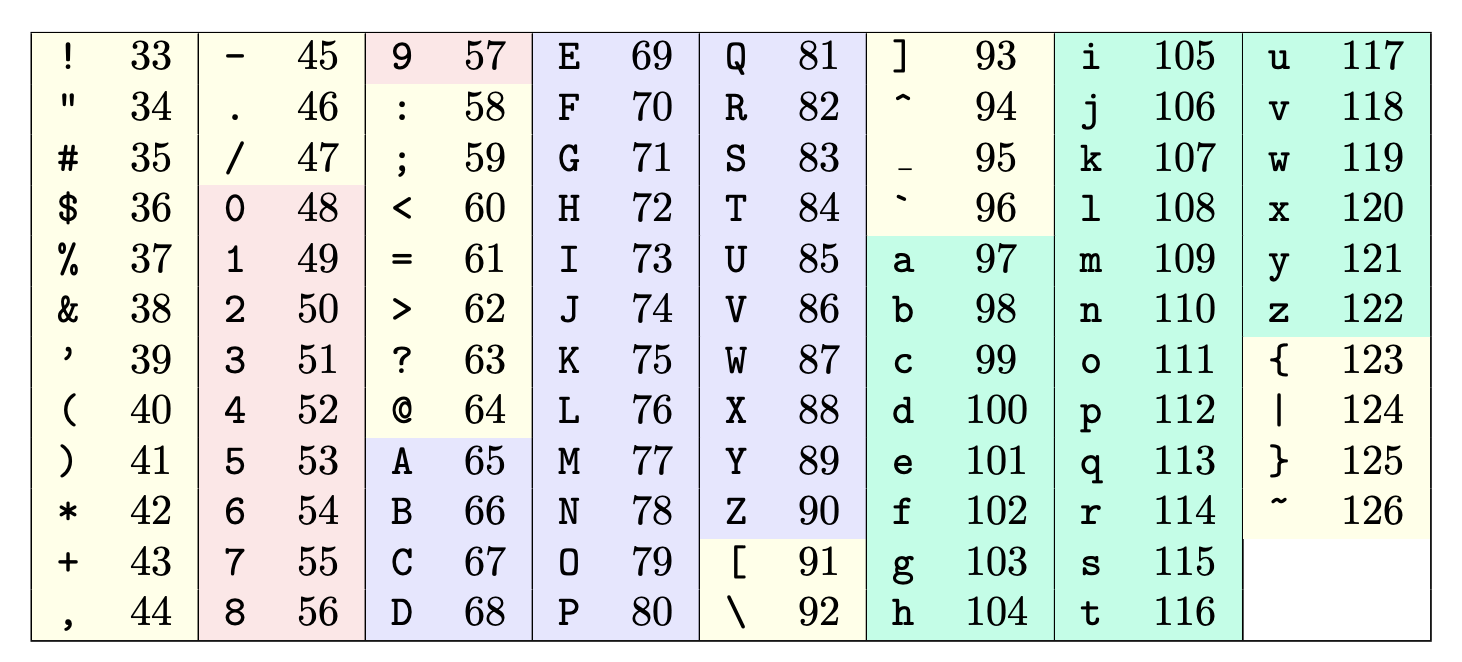
\includegraphics[width=\linewidth]{ASCII.png}

	\begin{multicols*}{2} % 开始双栏，数字 2 表示分两栏

		\subsection{初始化模板}

		\begin{minted}{cpp}
// teamname: Gospel_rock
/**
 * Problem: ${PROBLEM_NAME}
 * Contest: ${PROBLEM_GROUP_NAME}
 * Judge: ${ONLINE_JUDGE_NAME}
 * URL: ${PROBLEM_URL}
 * Created: ${YEAR}-${MONTH}-${DAY} ${HOUR}:${MINUTE}:${SECOND}
 * Author: Gospel_rock
 * My blog: https://znzryb.com/
 * 
 * Powered by AutoCp https://github.com/Pushpavel/AutoCp
 */

#include <bits/stdc++.h>
#define all(vec) vec.begin(), vec.end()
#define lson(o) (o << 1)
#define rson(o) (o << 1 | 1)
#define SZ(a) ((long long)a.size())
#define fsp(x) fixed << setprecision(x)
#define debug(x) cerr << "[" << #x << "]" << ": " << x << "\n"
#define cend cerr << "\n---------------------------------------------------\n"
#define cEnd cerr << "\n***************************************************\n"

using namespace std;

using ll = long long;
using ull = unsigned long long;
using DB = long double;
using i128 = __int128;
using CD = complex<double>;

static constexpr ll MAXN = (ll)1e6 + 10, INF = (1ll << 61) - 1;
static constexpr ll mod = 998244353;  // (ll)1e9+7;
static constexpr double eps = 1e-8;
// 不用 M_PI: 后者是 POSIX 扩展, glibc <cmath> 严格模式会 undef
const long double PI = acosl(-1.0);

ll lT, testcase;

/*
 *
 */

ll N;

void Solve() {
	cin >> N;
}

signed main() {
	ios::sync_with_stdio(false);
	cin.tie(nullptr);
	cout.tie(nullptr);
#ifdef LOCAL
	cout.setf(ios::unitbuf); // 无缓冲流，方便我们调试
#endif

	cin >> lT;
	for (testcase = 1; testcase <= lT; ++testcase)
		Solve();
	return 0;
}

/*

*/
		\end{minted}

		这个 \texttt{debug(x)} 是简版宏：单参数、直接 \texttt{cerr << x}，要求 \texttt{x} 支持 \texttt{operator<<}（基本类型 / \texttt{string} 都 OK，\texttt{vector<T>} 等容器不能直接打）。不再做 \texttt{LOCAL/非 LOCAL} 切换——OJ 上 stderr 通常不影响判分，留着也无伤大雅；介意的话提交前手动把 \texttt{debug(...)} 行删了或包成 \texttt{\#ifdef LOCAL} 即可。容器调试请用 range-for 手写循环。

		\subsection{CMake 配置}

		\subsubsection{Sanitizer 小技巧}

		有些越界或未定义行为问题，仅开 \texttt{address} 不一定能完整暴露。实践中建议同时开启 \texttt{address + undefined}，并保留帧指针，方便定位调用栈。

		\begin{minted}[highlightlines={9,10}]{cmake}
cmake_minimum_required(VERSION 3.31)
project(Edu_CF_186)

set(CMAKE_CXX_STANDARD 20)

add_executable(Edu_CF_186 main.cpp)

add_compile_definitions(LOCAL)
add_compile_options(-fsanitize=address,undefined -fno-omit-frame-pointer)
add_link_options(-fsanitize=address,undefined)

# 这个不要随便启用，启用后可能 debug 示数不可信
# add_compile_definitions(_GLIBCXX_DEBUG)

add_executable(A_New_Year_String "src/A_New_Year_String.cpp")
add_executable(B_New_Year_Cake "src/B_New_Year_Cake.cpp")
add_executable(odt_callback_bench "speed test/odt_callback_bench.cpp")
target_compile_options(odt_callback_bench PRIVATE "SHELL:${CMAKE_CXX_FLAGS_RELEASE}")
		\end{minted}

		\subsubsection{Cmake Release 配置小技巧}

		这个写法的主要目的有两个：一是只给特定目标启用 \texttt{Release} 进行性能测试，二是避免在 GUI 里把全局配置切到 \texttt{Release} 后忘记切回 \texttt{Debug}，进而出现调试信息异常、断点行为不符合预期等问题。

		\begin{minted}{cmake}
add_executable(odt_callback_bench "speed test/odt_callback_bench.cpp")
target_compile_options(odt_callback_bench PRIVATE "SHELL:${CMAKE_CXX_FLAGS_RELEASE}")
		\end{minted}

		\subsection{本地手测时怎么发 EOF}

		本地跑 \mintinline{cpp}{while (cin >> x)} / \mintinline{cpp}{while (scanf("\%d",&x) != EOF)} 这类按 EOF 终止的 CP 代码，手动在终端输完样例后要发 EOF 让 stdin 关流，否则程序一直阻塞读不到末尾。**EOF 的发送键在不同系统/终端里不一样**：

		\begin{itemize}
			\item \textbf{macOS / Linux 真终端}：\texttt{Ctrl-D}（在空输入行上按）。
			\item \textbf{Windows \texttt{cmd} / PowerShell}：\texttt{Ctrl-Z} 后按 \texttt{Enter}。
			\item \textbf{WSL / Git Bash on Windows}：\texttt{Ctrl-D}（同 Unix）。
			\item \textbf{CLion / VSCode Run 控制台}：跟底层 shell 走，mac/Linux $\Rightarrow$ \texttt{Ctrl-D}，Windows $\Rightarrow$ \texttt{Ctrl-Z}+\texttt{Enter}。
		\end{itemize}

		\textbf{两个坑}：

		\begin{itemize}
			\item \texttt{Ctrl-D} 只有在\textbf{空输入行}上才发 EOF；当前行已经敲了字符时，\texttt{Ctrl-D} 只把缓冲 flush 一次，要再按一次才真关流。
			\item CLion / VSCode 内嵌的 Run / Debug 控制台不是真 TTY，有的版本不响应 \texttt{Ctrl-D}——这时改用文件重定向喂输入：\mintinline{bash}{./a.out < in.txt}，或者直接用 heredoc：

\begin{minted}{bash}
./a.out << 'EOF'
3
1 2 3
EOF
\end{minted}
		\end{itemize}

	\end{multicols*} % 结束双栏

	\subsection{CLion 常用功能与快捷键（默认 keymap）}

	赛场 / 平时最常用的几个 CLion 操作与默认快捷键如下（赛场机一律 Windows / Linux，故只列这一套绑定）。\textbf{Run context configuration} 指「运行光标当前所在的那个目标」——多目标 CMake 工程里免去手动切下拉框，直接跑当前打开的这道题；\textbf{Reformat Code} 是一键格式化当前文件 / 选区；\textbf{Rename} 是语义级重命名，改变量 / 函数名时所有引用一起改，比全文替换安全（不会误伤字符串和同名的别的符号）。快捷键随 keymap 版本略有出入，忘了就用 \textbf{Find Action}（\texttt{Ctrl+Shift+A}）搜功能名，弹出项右侧直接显示当前绑定。

	\begin{center}
		\begin{tabular}{l|l}
			\hline
			功能 & Windows / Linux \\
			\hline
			Run context configuration（跑光标所在目标） & \texttt{Ctrl+Shift+F10}    \\
			\hline
			Run（当前选中的配置）                       & \texttt{Shift+F10}         \\
			\hline
			Debug（当前选中的配置）                     & \texttt{Shift+F9}          \\
			\hline
			Build Project（只编译不跑）                 & \texttt{Ctrl+F9}           \\
			\hline
			Reformat Code（格式化当前文件 / 选区）       & \texttt{Ctrl+Alt+L}        \\
			\hline
			Rename（重命名符号 + 所有引用）              & \texttt{Shift+F6}          \\
			\hline
			注释 / 取消注释行                           & \texttt{Ctrl+/}            \\
			\hline
			复制当前行 / 选区                           & \texttt{Ctrl+D}            \\
			\hline
			删除整行                                   & \texttt{Ctrl+Y}            \\
			\hline
			上 / 下移当前行                            & \texttt{Alt+Shift+Up/Down} \\
			\hline
			Find Action（搜任意功能 / 快捷键）           & \texttt{Ctrl+Shift+A}      \\
			\hline
		\end{tabular}
	\end{center}

	\subsection{CLion 语言引擎：赛场机上先切 Nova}

	CLion 有两套\textbf{语言引擎}，补全 / 高亮 / 跳转的行为由它决定，**赛场机开机后第一件事就是确认切到 Nova**：

	\begin{itemize}
		\item \textbf{CLion Classic}——核心 code insight（补全、高亮）由 \textbf{clangd} 提供，另有一个 legacy 引擎负责重构等其余功能。
		\item \textbf{CLion Nova}——换成 \textbf{ReSharper C++ / Rider C++ 引擎}，核心功能\textbf{完全不走 clangd}（JetBrains 的 clangd fork 仍在后台跑，但只管 ClangFormat / Clang-Tidy / MISRA / 数据流分析）。
	\end{itemize}

	两套是彼此独立的实现，所以「同一个 IDE、同一份代码，两台机补全行为不一样」很正常——换引擎等于换了整个语言前端。对竞赛影响最大的一处差异：

	\begin{center}
		\begin{tabular}{l|l|l}
			\hline
			输入                                & CLion Nova                                     & CLion Classic                        \\
			\hline
			\mintinline{cpp}{vec} + \texttt{Enter}  & \mintinline{cpp}{vector<>}（光标落在尖括号中间） & \mintinline{cpp}{vector}（尖括号自己敲） \\
			\hline
			\mintinline{cpp}{#inc} + \texttt{Enter} & \mintinline{cpp}{#include}（只有指令）           & \mintinline{cpp}{#include <>} + 头文件列表 \\
			\hline
		\end{tabular}
	\end{center}

	第一行是\textbf{选 Nova 的主要理由}：竞赛里 \mintinline{cpp}{vector} / \mintinline{cpp}{map} / \mintinline{cpp}{priority_queue} 满屏都是，少敲一对尖括号累积起来很可观。Classic 这边\textbf{既不是 bug 也没有开关}——clangd 只对\textbf{函数模板}（且模板参数推导不出来时）补尖括号，\textbf{类模板一律不补}：C++17 起有了 CTAD，\mintinline{cpp}{vector v{1, 2};} 本身就合法，IDE 判断不出你要不要那对尖括号，索性不插（见 JetBrains issue \texttt{CPP-154}）。

	第二行是反向的坑，切之前知道一下：Nova 目前\textbf{没有} \mintinline{cpp}{#include <...>} 的补全，只补一个光秃秃的 \mintinline{cpp}{#include}（issue \texttt{CPP-47569}，仍 open）。竞赛基本只写一行 \mintinline{cpp}{#include <bits/stdc++.h>}，影响不大。

	\textbf{怎么切}（两条路径任选其一）：

	\begin{enumerate}
		\item 右侧工具栏齿轮（\textbf{IDE and Project Settings}）$\rightarrow$ \textbf{Switch to Nova Engine} $\rightarrow$ \textbf{Enable and Restart}。
		\item \textbf{Settings} $\rightarrow$ \textbf{Advanced Settings} $\rightarrow$ 勾上 \textbf{Use the ReSharper C++ language engine (CLion Nova)} $\rightarrow$ \textbf{Apply}。
	\end{enumerate}

	切换要重启 IDE 并重新解析项目。竞赛工程就几个 \texttt{.cpp}，几秒的事，但\textbf{务必在热身赛就切好}，别等开赛才发现要重启。IDE 设置是每台机独立的，赛场机每次重装镜像都要重切一次。

	\textbf{版本背景}：Nova 自 \textbf{CLion 2025.3} 起是所有用户的默认引擎；\textbf{2026.2} 把 Classic 从 IDE 里 unbundle 成可选插件（\texttt{C/C++ Language Support via Classic Engine}）；\textbf{2026.3}（2026 年 11 月）是最后一个兼容 Classic 的稳定版。所以赛场机若装了较新版本，默认就是 Nova、无需操心；只有还能看到「选不选 Nova」的机器（版本大致在 2024.2--2026.1 之间）才需要手动切。

	\subsection{Windows：禁用 \texttt{Shift} 切换中英文输入}

	Windows 赛场机上敲代码，误碰 \texttt{Shift}（打大写、打符号松手稍慢）就会被输入法切到中文模式，接着敲出一串全角字符——开赛前先把这个切换键关掉。

	\subsubsection{微软拼音（系统自带，Win10 逐步截图）}

	\begin{enumerate}
		\item 开始菜单 → \textbf{设置}：
		      \begin{center}
			      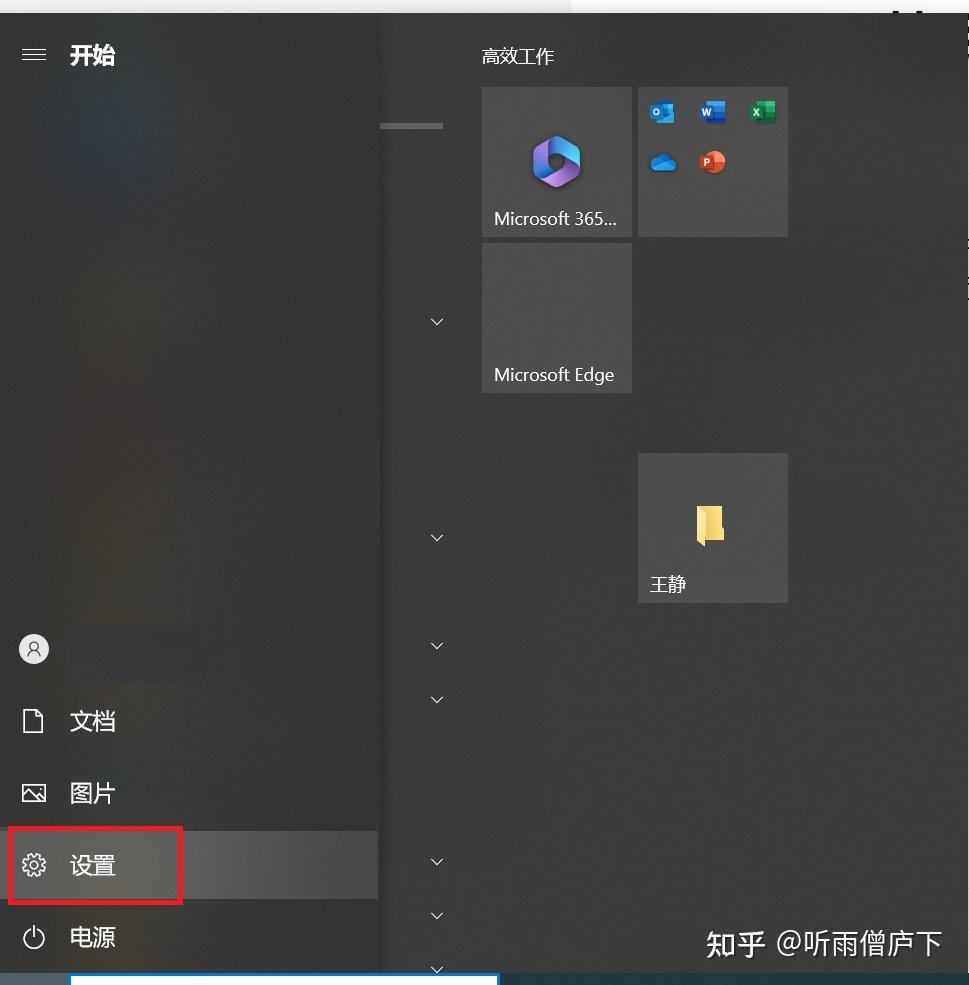
\includegraphics[width=0.42\linewidth]{image/ime_win10_01_开始菜单设置.jpg}
		      \end{center}
		\item 进入\textbf{时间和语言}：
		      \begin{center}
			      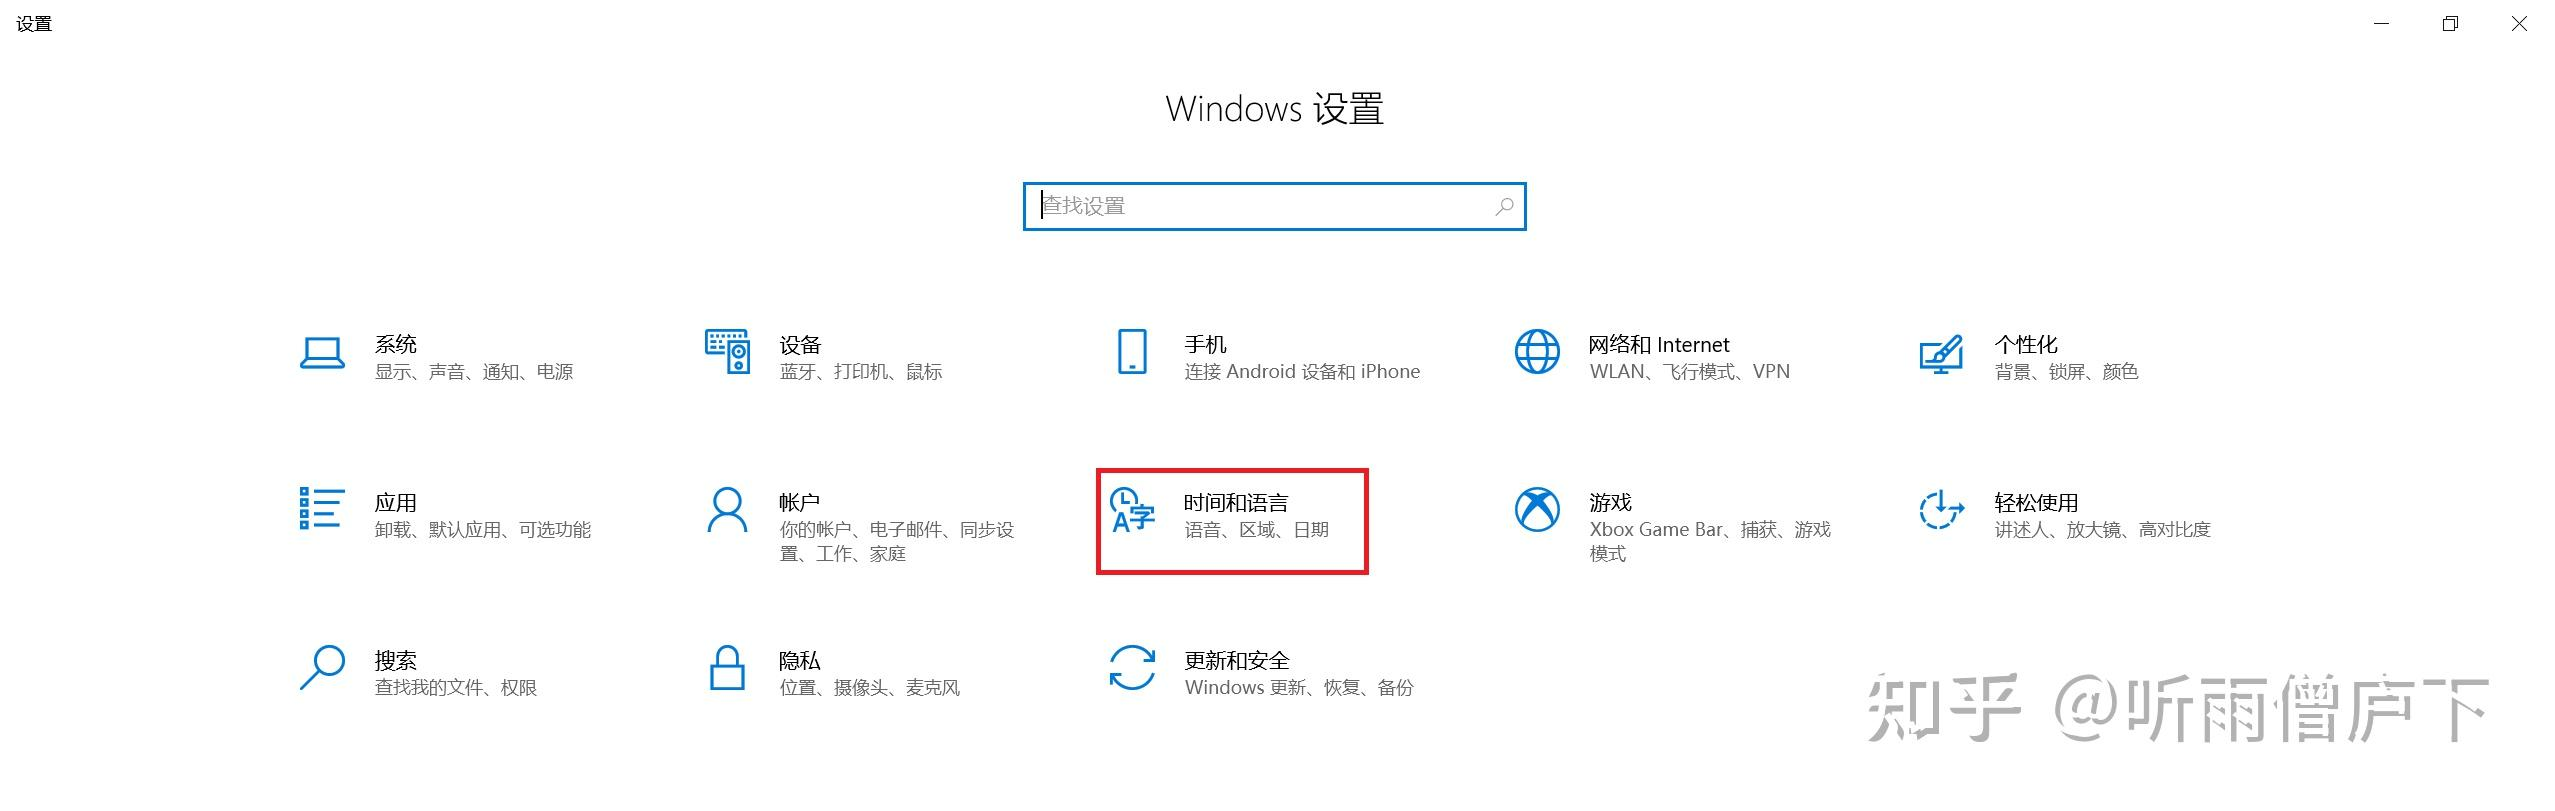
\includegraphics[width=0.85\linewidth]{image/ime_win10_02_时间和语言.jpg}
		      \end{center}
		\item 左侧栏切到\textbf{语言}：
		      \begin{center}
			      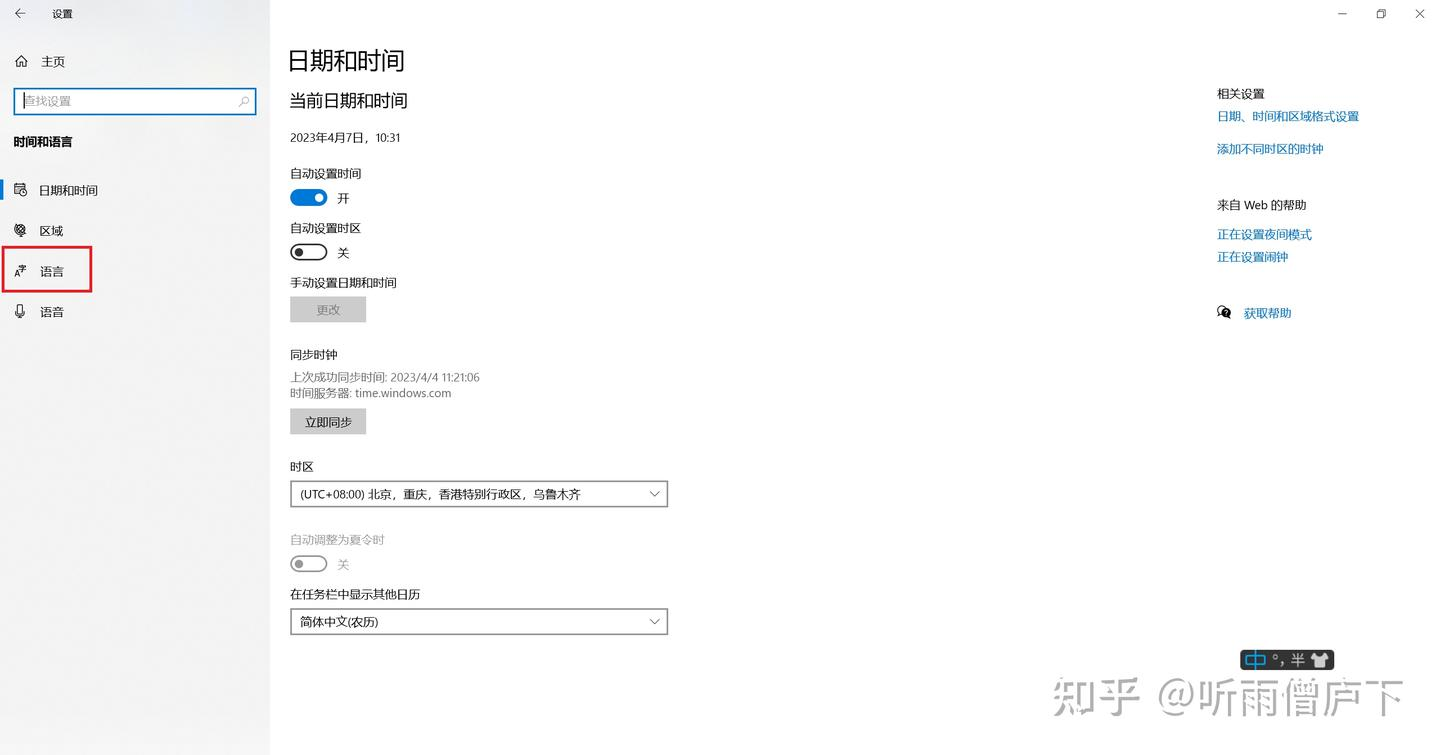
\includegraphics[width=0.75\linewidth]{image/ime_win10_03_左栏语言.jpg}
		      \end{center}
		\item 「首选语言」列表里点\textbf{中文(简体，中国)}：
		      \begin{center}
			      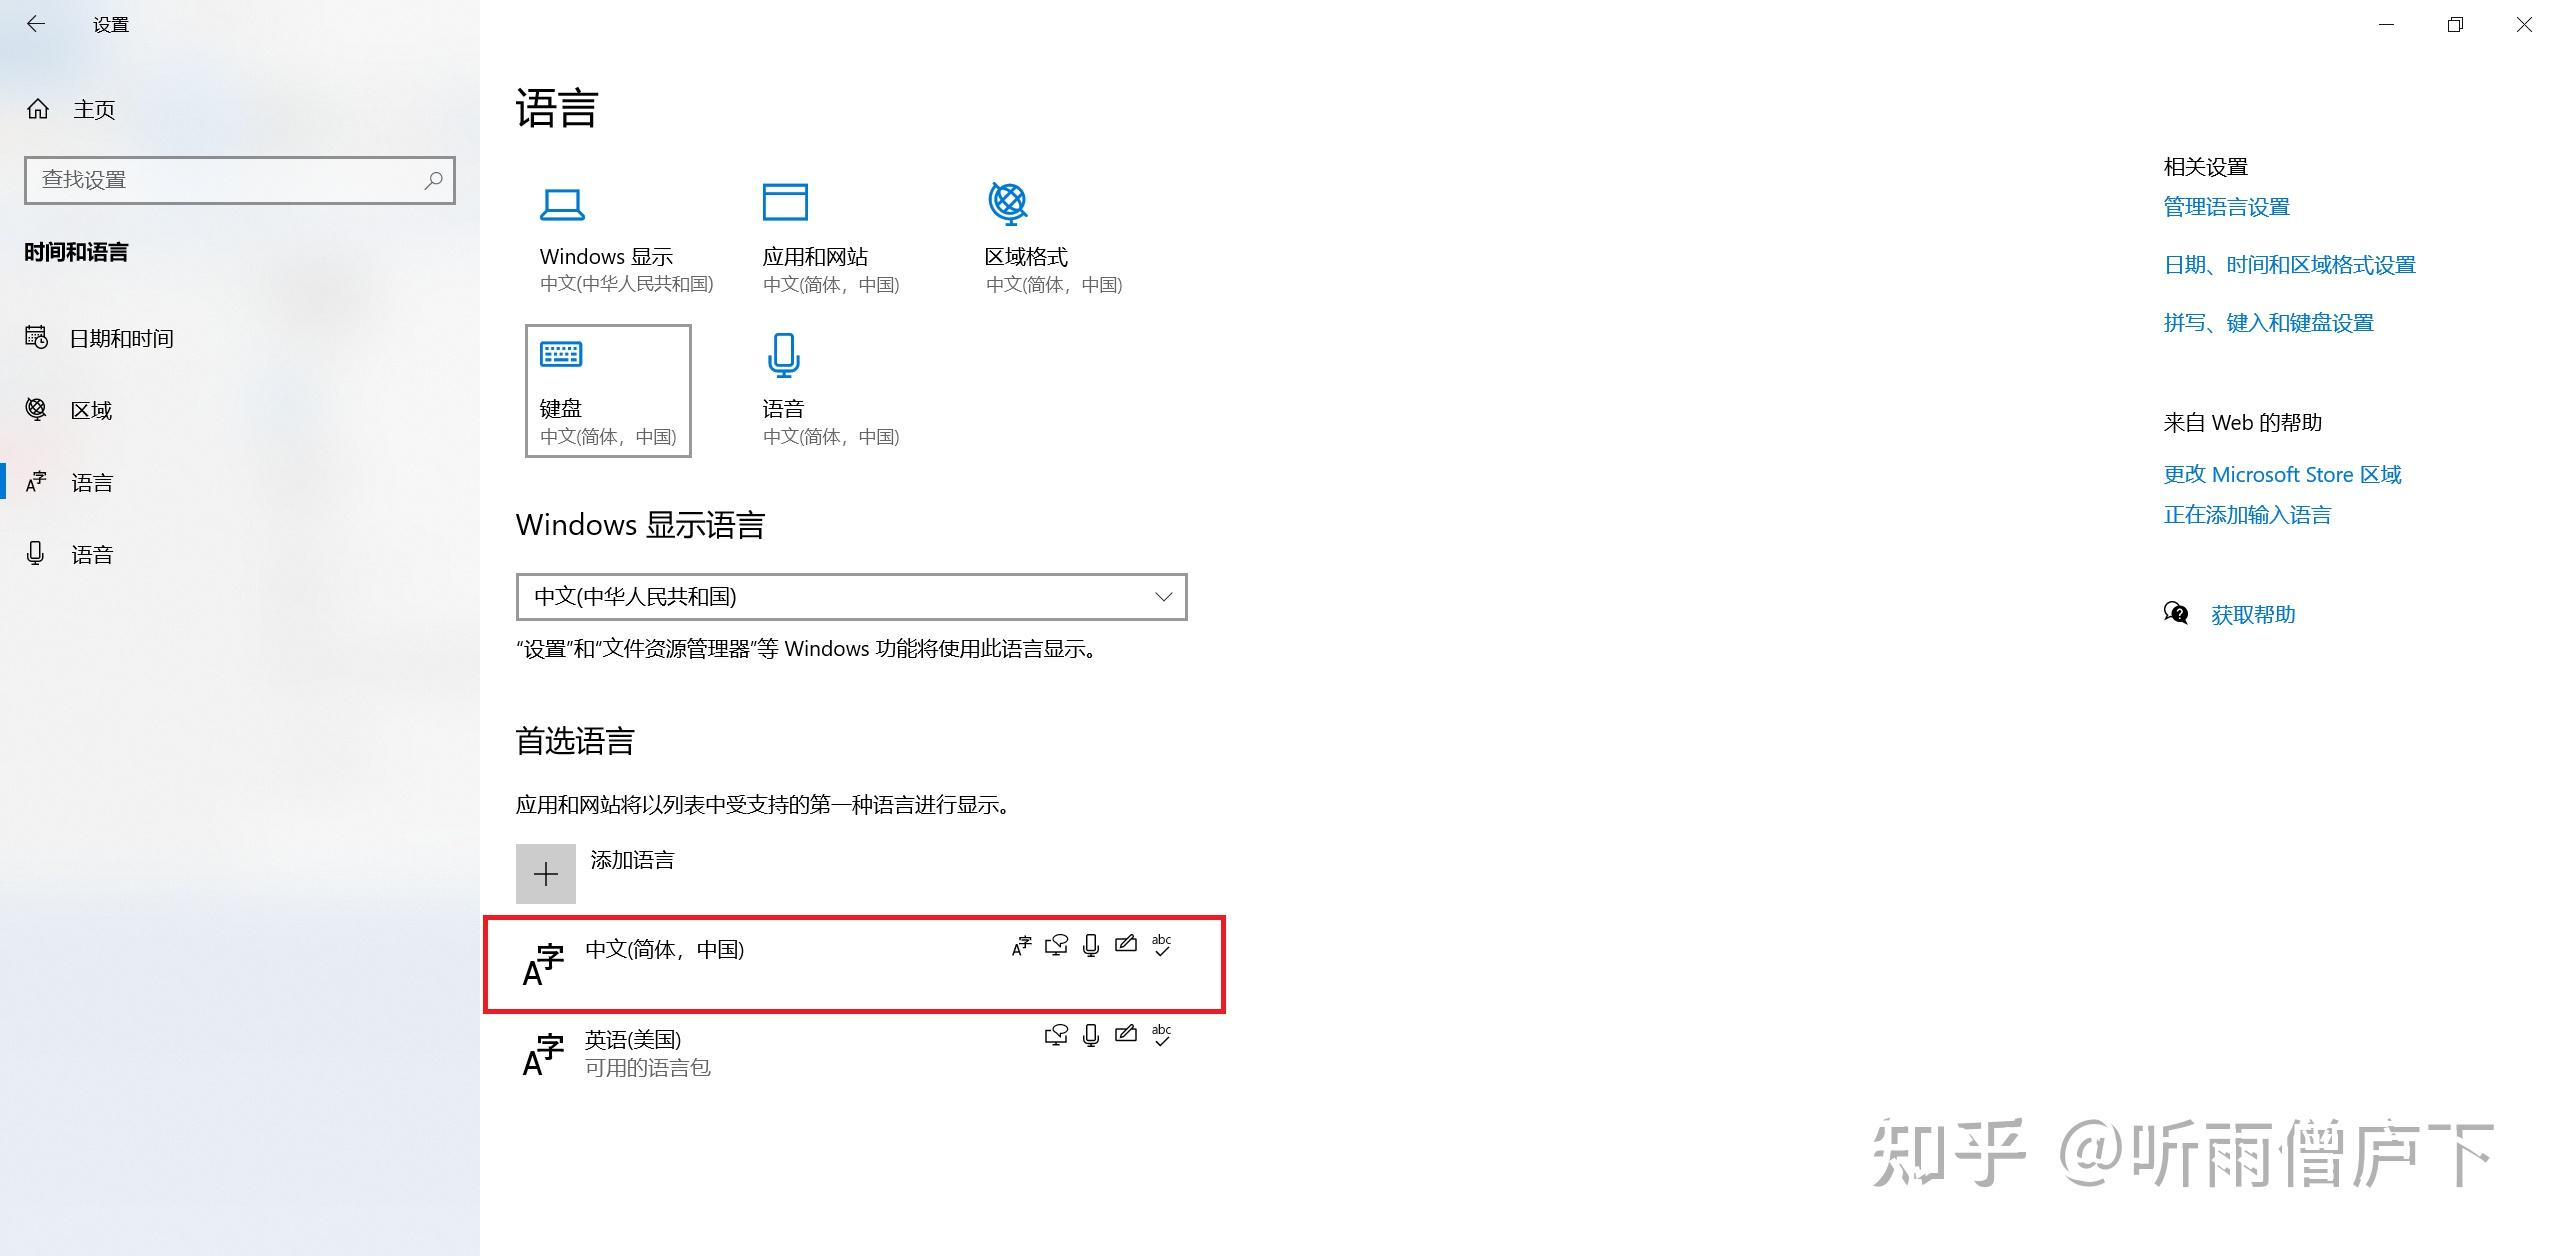
\includegraphics[width=0.85\linewidth]{image/ime_win10_04_首选语言点中文.jpg}
		      \end{center}
		\item 点展开出来的\textbf{选项}按钮：
		      \begin{center}
			      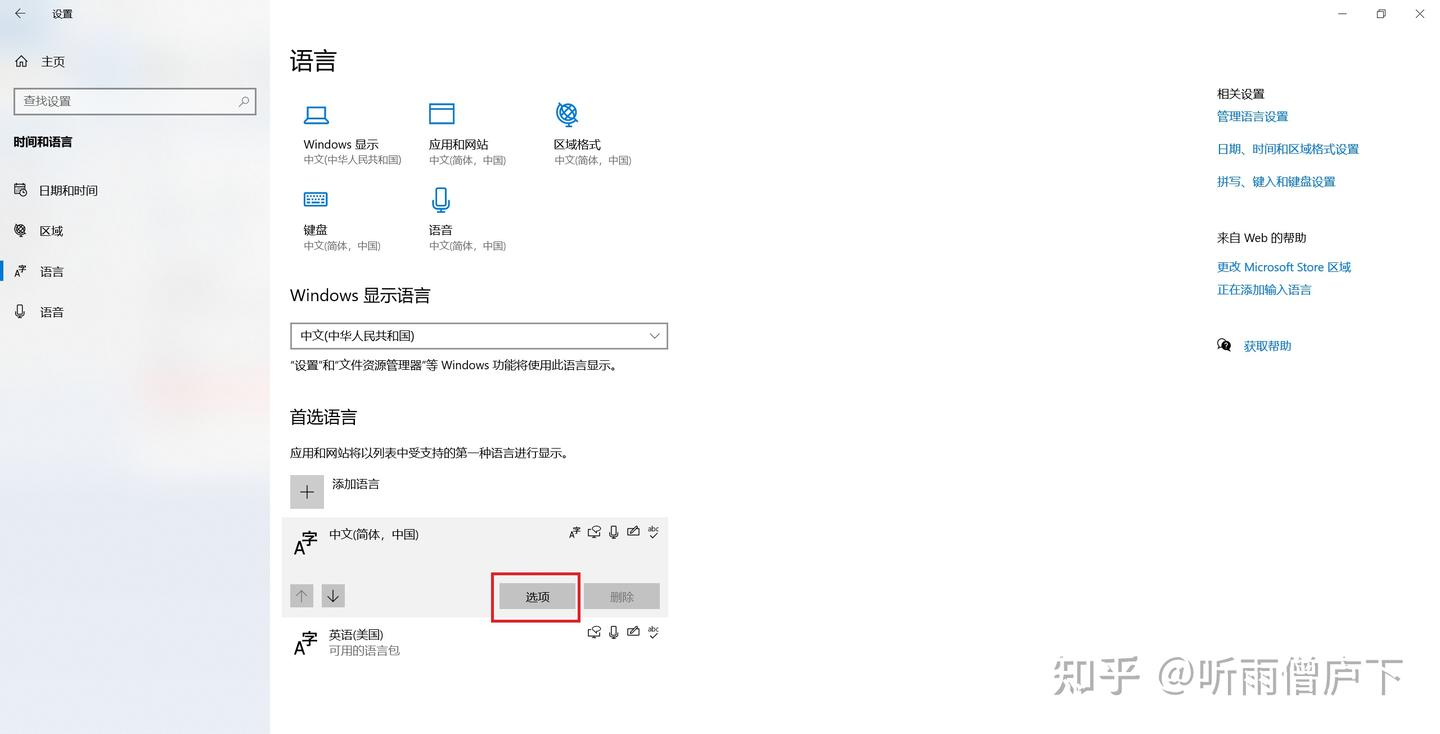
\includegraphics[width=0.75\linewidth]{image/ime_win10_05_选项按钮.jpg}
		      \end{center}
		\item 键盘列表里点\textbf{微软拼音} → 进入\textbf{按键}：
		      \begin{center}
			      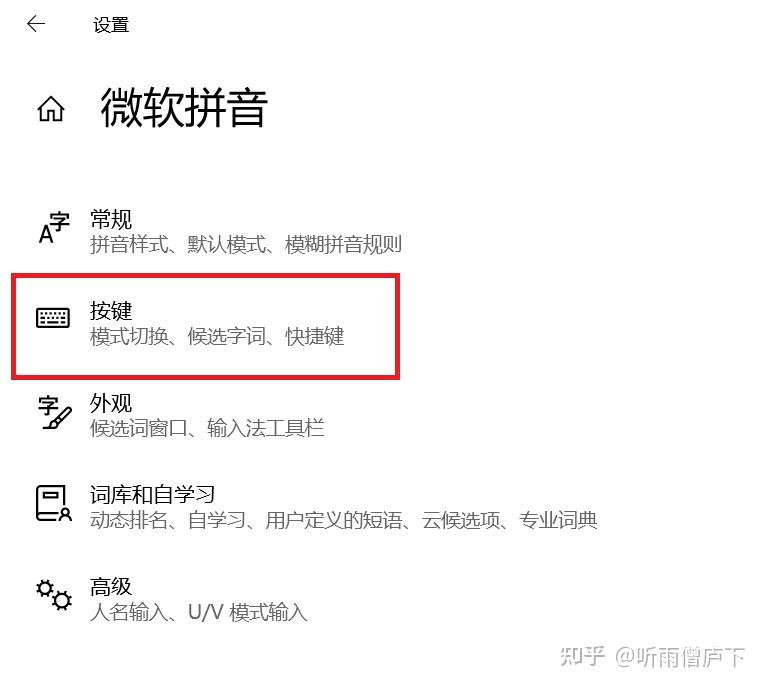
\includegraphics[width=0.45\linewidth]{image/ime_win10_06_微软拼音按键.jpg}
		      \end{center}
		\item 「中/英文模式切换」里\textbf{把 \texttt{Shift} 的勾去掉}（保留 \texttt{Ctrl + 空格键}，这就是之后手动切中英文的键）：
		      \begin{center}
			      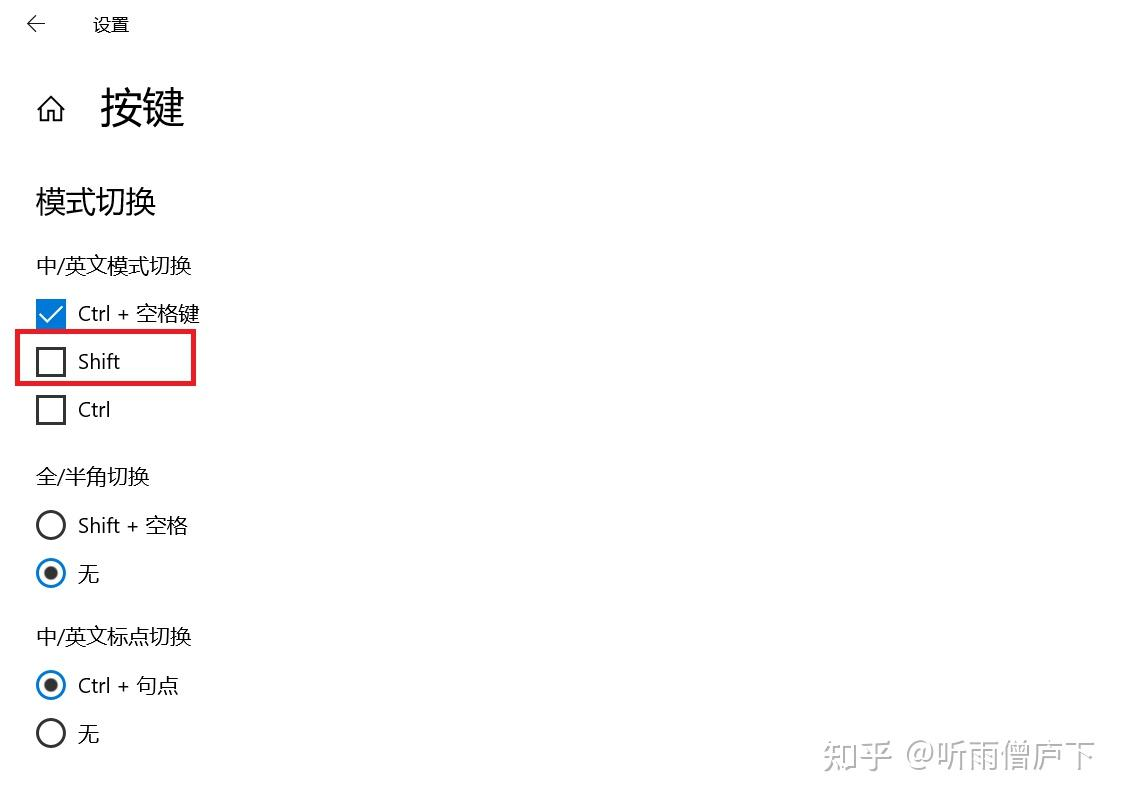
\includegraphics[width=0.55\linewidth]{image/ime_win10_07_取消Shift勾选.jpg}
		      \end{center}
	\end{enumerate}

	改完后 \texttt{Shift} 只做普通修饰键；切中英文用 \texttt{Ctrl + Space}，切输入法 / 语言用 \texttt{Win + Space}。Win11 路径名稍有不同：设置 → 时间和语言 → \textbf{语言和区域} → 中文右侧「…」→ 语言选项 → 微软拼音 → 键盘选项 → 按键，最后一步相同。

	\subsubsection{搜狗输入法}

	\begin{enumerate}
		\item 任务栏搜狗图标打开工具面板 → \textbf{更多设置(P)}：
		      \begin{center}
			      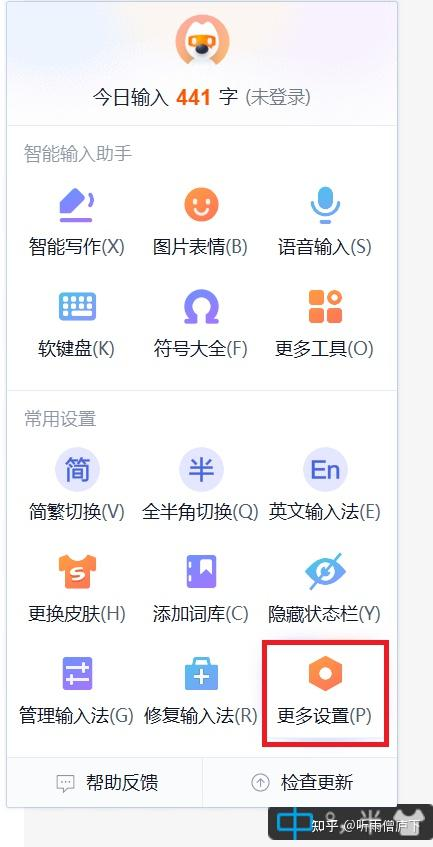
\includegraphics[width=0.3\linewidth]{image/ime_sogou_01_更多设置.jpg}
		      \end{center}
		\item 属性设置 → \textbf{按键} → 「中英切换」选\textbf{无}（不想彻底禁可选 \texttt{Ctrl}）：
		      \begin{center}
			      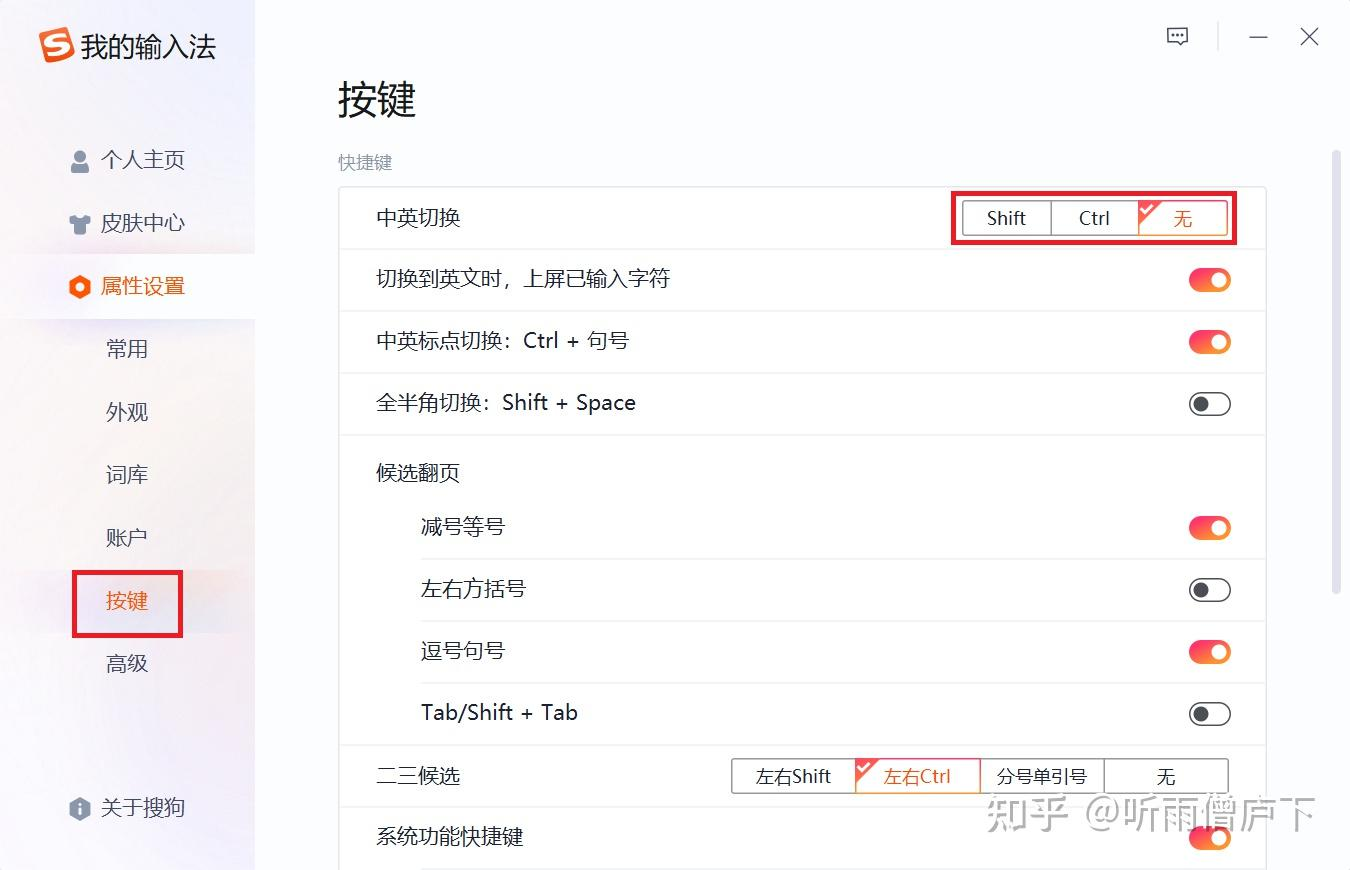
\includegraphics[width=0.6\linewidth]{image/ime_sogou_02_中英切换选无.jpg}
		      \end{center}
	\end{enumerate}

	QQ / 百度输入法路径类似，都在「按键设置」里。

	\textbf{更省事的做法}（比赛全程不需要中文输入时）：直接在上面第 4 步的语言列表里\textbf{删掉中文输入法}或把默认语言切到 \texttt{ENG}，\texttt{Shift} 就完全没有切换语义了。快速定位入口：开始菜单搜「输入法」→「编辑语言和键盘选项」。






		\begin{center}
		\section{基础数学}
	\end{center}

	\begin{multicols*}{2} % 开始双栏，数字 2 表示分两栏

		\subsection{快速幂}


		\begin{minted}{cpp}
// 在 k<=0 的时候返回 1
ll binpow(ll a,ll k,const ll &p=mod){
	ll res=1;
	a%=p;
	while(k>0){
		if((k&1)==1) res=a*res%p;
		a=a*a%p;
		k>>=1;
	}
	return res;
}
		\end{minted}

		\subsection{矩阵快速幂}

		注意，我们这个东西依赖于后面的这个\textcolor{red}{\textbf{自动取模类}}，所以代码还是比较长的。

		\begin{minted}{cpp}
/*
* 2025/11/5 https://www.luogu.com.cn/record/245403611 矩阵快速幂模版题
* 2025/11/5 https://www.luogu.com.cn/record/245411884 P1939 矩阵加速（数列）
* 2026/3/4 去除了过时的宏定义和没有意义的压行
*/
template<class T>
struct Matrix {
	int n, m;
	vector<vector<T> > a; // 1-based

	Matrix() : n(0), m(0) {
	}

	Matrix(int n_, int m_, const T &val = T()) {
		assign(n_, m_, val);
	}

	// 用 1-based 的 vv 构造
	Matrix(const vector<vector<T> > &vv) { load(vv); }

	// vv.size() == n+1, vv[1].size() == m+1
	void load(const vector<vector<T> > &vv) {
		n = (int) vv.size() - 1;
		m = n ? (int) vv[1].size() - 1 : 0;
		a = vv;
	}

	void assign(int n_, int m_, const T &val = T()) {
		n = n_;
		m = m_;
		a.assign(n + 1, vector<T>(m + 1, val));
	}

	// 重载
	vector<T> &operator[](int i) { return a[i]; }
	const vector<T> &operator[](int i) const { return a[i]; }

	// += 负责真正干活
	Matrix &operator+=(const Matrix &rhs) {
		assert(n == rhs.n && m == rhs.m);
		for (int i = 1; i <= n; ++i) {
			for (int j = 1; j <= m; ++j) {
				a[i][j] += rhs[i][j];
			}
		}

		return *this;
	}

	// + 基于 +=
	Matrix operator+(const Matrix &rhs) const {
		Matrix res(*this);
		res += rhs;
		return res;
	}

	Matrix &operator-=(const Matrix &rhs) {
		assert(n == rhs.n && m == rhs.m);
		for (int i = 1; i <= n; ++i) {
			for (int j = 1; j <= m; ++j) {
				a[i][j] -= rhs[i][j];
			}
		}

		return *this;
	}

	Matrix operator-(const Matrix &rhs) const {
		Matrix res(*this);
		res -= rhs;
		return res;
	}

	Matrix &operator*=(const Matrix &rhs) {
		*this = (*this) * rhs;
		return *this;
	}

	Matrix operator*(const Matrix &rhs) const {
		assert(m == rhs.n);
		Matrix res(n, rhs.m, T());
		for (int i = 1; i <= n; ++i) {
			for (int k = 1; k <= m; ++k) {
				if (a[i][k] != T()) {
					for (int j = 1; j <= rhs.m; ++j) {
						res[i][j] += a[i][k] * rhs[k][j];
					}
				}
			}
		}
		return res;
	}

	static Matrix identity(int n) {
		Matrix I(n, n, T());
		for (int i = 1; i <= n; ++i) I[i][i] = T(1);
		return I;
	}

	friend ostream &operator<<(ostream &os, const Matrix &ma) {
		for (int i = 1; i <= ma.n; ++i) {
			for (int j = 1; j <= ma.m; ++j) {
				os << ma[i][j] << " ";
			}
			os << "\n";
		}
		return os;
	}
};

// 矩阵快速幂：必须是方阵
template<class T>
Matrix<T> mat_pow(Matrix<T> base, long long exp) {
	assert(base.n == base.m);
	Matrix<T> res = Matrix<T>::identity(base.n);
	while (exp > 0) {
		if (exp & 1) res = res * base;
		base = base * base;
		exp >>= 1;
	}
	return res;
}
		\end{minted}

		\subsubsection{矩阵快速幂加速递推}
		已知一个数列 $a$，它满足：
		\[
			a_x = \begin{cases}
					  1 & x \in \{1,2,3\} \\ a_{x-1} + a_{x-3} & x \geq 4
			\end{cases}
		\]
		求 $a$ 数列的第 $n$ 项对 $10^9+7$ 取余的值。

		对于递推式 $a_x = a_{x-1} + a_{x-3}$，因为递推涉及到了前 $3$ 项的状态，我们可以构造一个大小为 $3 \times 1$ 的状态列向量 $\begin{bmatrix}
																																   a_x \\ a_{x-1} \\ a_{x-2}
		\end{bmatrix}$。

		根据递推关系，我们可以将其展开为矩阵乘法的形式，寻找转移矩阵 $T$：
		\[
			\begin{aligned}
				a_x     & = 1 \cdot a_{x-1} + 0 \cdot a_{x-2} + 1 \cdot a_{x-3} \\
				a_{x-1} & = 1 \cdot a_{x-1} + 0 \cdot a_{x-2} + 0 \cdot a_{x-3} \\
				a_{x-2} & = 0 \cdot a_{x-1} + 1 \cdot a_{x-2} + 0 \cdot a_{x-3}
			\end{aligned}
		\]
		通过提取系数，可以得出转移矩阵 $T$：
		\[
			\begin{bmatrix}
				a_x \\ a_{x-1} \\ a_{x-2}
			\end{bmatrix} = \begin{bmatrix}
								1 & 0 & 1 \\ 1 & 0 & 0 \\ 0 & 1 & 0
			\end{bmatrix} \begin{bmatrix}
							  a_{x-1} \\ a_{x-2} \\ a_{x-3}
			\end{bmatrix}
		\]
		(这里就是普通的矩阵乘法，按照矩阵乘法规则展开，上式和下式是等价的)
		\\
		初始状态列向量为 $V = \begin{bmatrix}
								  a_3 \\ a_2 \\ a_1
		\end{bmatrix} = \begin{bmatrix}
							1 \\ 1 \\ 1
		\end{bmatrix}$。

		将转移矩阵 $T$ 自乘 $n-1$ 次后，再乘以初始向量 $V$，即可得到最终状态：
		\[
			T^{n-1} V = \begin{bmatrix}
							1 & 0 & 1 \\ 1 & 0 & 0 \\ 0 & 1 & 0
			\end{bmatrix}^{n-1} \begin{bmatrix}
									a_3 \\ a_2 \\ a_1
			\end{bmatrix} = \begin{bmatrix}
								a_{n+2} \\ a_{n+1} \\ a_n
			\end{bmatrix}
		\]
		由此可见，经过 $n-1$ 次状态转移后，底部的元素恰好从 $a_1$ 递推变为了 $a_n$。因此结果矩阵的第 3 行第 1 列即为所求的 $a_n$（在代码中由于加入了空的 \verb|{}| 占位使下标从 1 开始，对应为 \verb|mat[3][1]|）。


		\begin{minted}{cpp}
void Solve() {
	ll n;
	cin >> n;
	vector<vector<modi> > A{
				{},     // 递推矩阵
				{{}, 1, 0, 1},// fn = fn-1 + 0*fn-2 + fn-3
				{{}, 1, 0, 0},
				{{}, 0, 1, 0}
			},
			B = {       // 原向量 v（也可以认为是一个矩阵）
				{},
				{{}, 1}, // a3
				{{}, 1}, // a2
				{{}, 1}  // a1
			};
	Matrix mat(A),matb(B);
	mat = mat_pow(mat, n-1);
	mat*=matb; // 递推矩阵T*原向量 v
	// a1递推n-1次，是这个 an
	cout << mat[3][1] << "\n";
}
		\end{minted}

		对于递推式 $S_{n}=22S_{n-1}-S_{n-2}$，我们可以将其转化为矩阵乘法的形式来加速计算。

		首先构造状态列向量 $\begin{bmatrix}
								S_n \\ S_{n-1}
		\end{bmatrix}$，根据递推关系可以得出转移矩阵 $T$：
		\[
			\begin{bmatrix}
				S_n \\ S_{n-1}
			\end{bmatrix} = \begin{bmatrix}
								22 & -1 \\ 1 & 0
			\end{bmatrix} \begin{bmatrix}
							  S_{n-1} \\ S_{n-2}
			\end{bmatrix}
		\]
		初始状态列向量为 $V = \begin{bmatrix}
								  S_2 \\ S_1
		\end{bmatrix} = \begin{bmatrix}
							482 \\ 22
		\end{bmatrix}$。

		将转移矩阵 $T$ 自乘 $n-1$ 次后，再乘以初始向量 $V$，即可得到最终状态：
		\[
			T^{n-1} V = \begin{bmatrix}
							22 & -1 \\ 1 & 0
			\end{bmatrix}^{n-1} \begin{bmatrix}
									S_2 \\ S_1
			\end{bmatrix} = \begin{bmatrix}
								S_{n+1} \\ S_n
			\end{bmatrix}
		\]
		由此可见，计算结果矩阵的第 2 行第 1 列即为所求的 $S_n$。代码中因为使用了一个空的 \verb|{}| 进行占位（即下标从 1 开始），所以对应的取值为 \verb|T[2][1]|。


		\begin{minted}{cpp}
vector<vector<modi> >
// 构造转移矩阵 T
// [ S_n   ] = [ 22 -1 ] * [ S_{n-1} ]
// [ S_{n-1} ]   [  1  0 ]   [ S_{n-2} ]
// 注意：用 {} 占位使得二维 vector 的下标从 1 开始
tmp={{},
	{{},22,-1},
	{{},1,0},
	};
Matrix T(tmp);

// 将转移矩阵自乘 n-1 次
T=mat_pow(T,n-1);

// 构造初始状态列向量 V
// V = [ S_2 ] = [ 482 ]
//     [ S_1 ]   [  22 ]
vector<vector<modi> > tmp2=
	{{},
	{{},482},
	{{},22},
	};
Matrix V(tmp2);

// 将转移矩阵和初始向量相乘：T^{n-1} * V
T*=V;

// 提取结果 S_n
// 经过 n-1 次转移后，结果列向量变为 [ S_{n+1} ]
//                               [ S_n     ]
// 故所求结果在第 2 行第 1 列（1-indexed）
modi res=T[2][1];
		\end{minted}

		\subsection{自动取模类}
		\begin{minted}{cpp}
// T: 底层存储类型 (uint32_t / uint64_t)
// MOD: 模数
// Wide: 乘法时用的更宽类型
template <class T, T MOD, class Wide = ull>
struct modint {
	T v;
	modint(ll x = 0) {
		ll t = x % (ll)MOD;
		if (t < 0) t += MOD;
		v = (T)t;
	}

	T val() const { return v; }

	modint& operator+=(const modint &o) {
		T x = v + o.v;
		if (x >= MOD) x -= MOD;
		v = x;
		return *this;
	}

	modint& operator-=(const modint &o) {
		T x = v >= o.v ? v - o.v : (T)(v + MOD - o.v);
		v = x;
		return *this;
	}

	modint& operator*=(const modint &o) {
		Wide t = (Wide)v * (Wide)o.v;
		v = (T)(t % MOD);
		return *this;
	}

	// 幂
	static modint powmod(modint a, ll e) {
		modint r = 1;
		while (e) {
			if (e & 1) r *= a;
			a *= a;
			e >>= 1;
		}
		return r;
	}

	// 逆元（假定 MOD 是质数）
	static modint inv(modint a) {
		return powmod(a, (ll)MOD - 2);
	}

	modint& operator/=(const modint &o) {
		return *this *= inv(o);
	}

	// 一元
	modint operator+() const { return *this; }
	modint operator-() const { return modint(0) - *this; }

	// 二元
	friend modint operator+(modint a, const modint &b) { return a += b; }
	friend modint operator-(modint a, const modint &b) { return a -= b; }
	friend modint operator*(modint a, const modint &b) { return a *= b; }
	friend modint operator/(modint a, const modint &b) { return a /= b; }

	friend bool operator==(const modint &a, const modint &b) { return a.v == b.v; }
	friend bool operator!=(const modint &a, const modint &b) { return a.v != b.v; }

	friend ostream& operator<<(ostream &os, const modint &x) {
		return os << x.v;
	}
	friend istream& operator>>(istream &is, modint &x) {
		ll t;
		if (!(is >> t)) return is;
		x = modint(t);
		return is;
	}
};
using modi=modint<uint32_t,mod>;
		\end{minted}

% 我们发现我们自己的那个模板也是线性递推的，因此就不需要这个板子了

% \subsection{预处理逆元（一个数的逆元）}

% 假设要求 $i$ 模 $p$（$p$ 为素数）的逆元，也就是计算 $i^{-1} \pmod p$。

% 首先我们进行带余除法，将 $p$ 分解为包含 $i$ 的形式。令 $q = \lfloor \frac{p}{i} \rfloor$ 为商，$r = p \bmod i$ 为余数，显然有：
% $$
% p = q \times i + r
% $$
% 将等式两边放到模 $p$ 意义下，左边的 $p$ 就变成了 $0$：
% $$
% 0 \equiv q \times i + r \pmod p
% $$
% 因为我们的目标是求出 $i$ 的逆元 $i^{-1}$，我们可以考虑在等式两边同时乘以 $i^{-1} \times r^{-1}$，这样能把 $i$ 和 $r$ 的逆元构造出来：
% $$
% 0 \equiv q \times r^{-1} + i^{-1} \pmod p
% $$
% 移项后，就把未知的 $i^{-1}$ 单独留在一边，用已知的 $r^{-1}$ 表示出来了：
% $$
% i^{-1} \equiv -q \times r^{-1} \pmod p
% $$
% 最后将 $q$ 和 $r$ 的定义代入回来，就得到了完整的递推式：
% $$
% i^{-1} \equiv -\lfloor \frac{p}{i} \rfloor \times (p \bmod i)^{-1} \pmod p
% $$
% 由于余数 $p \bmod i$ 必定严格小于 $i$，因此我们在从小到大递推求解时，$(p \bmod i)^{-1}$ 已经被计算过了，可以直接利用。

% 代码实现中，为了防止 $-q$ 取模产生负数，我们通常将其加上 $p$（即代码中的 \verb|mod - q|）再进行计算。

% 代码参考了 starsilk：

% \begin{minted}{cpp}
% 	inv[1] = 1;
% 	for (int i = 2; i < MAXN - 5; i++) {
% 		long long r = mod % i;
% 		long long q = mod / i;
% 		inv[i] = inv[r] * (mod - q) % mod;
% 	}
% \end{minted}

		\subsection{异或线性基（linear basis）}

		异或线性基用于解决在一个整数集合中，任意选取元素进行异或操作所能产生的数值组合问题。其核心原理基于线性代数中的向量空间，将整数的二进制表示看作位于 $\mathbb{F}_2$ 域（即模 $2$ 加法，等价于异或）上的向量。

		模板中各核心操作的理论基础如下：
		\begin{itemize}
			\item \textbf{插入（\texttt{insert}）}：本质是向极大线性无关组中添加新向量的过程。从高位到低位遍历，若当前数字的第 $i$ 位为 $1$，且该位已存在基底 $d_i$，则将数字异或 $d_i$ 以消去该位；若不存在基底，则将当前数字作为 $d_i$ 存入，插入成功。若最终数字变为 $0$，说明它可由已有基底线性表出。
			\item \textbf{查询最大值（\texttt{query\_max}）}：基于贪心思想。从高位到低位遍历，对于第 $i$ 位的基底 $d_i$，因为它是集合中唯一最高位为 $i$ 的基底，若当前答案异或 $d_i$ 后能变大，则必定选择异或。因为无论后面低位如何选择，都无法弥补当前第 $i$ 位错失的 $1$。
			\item \textbf{查询最小值（\texttt{query\_min}）}：如果在插入时出现过能被线性表出的数字（即能异或出 $0$），那么最小值就是 $0$；否则，由于基底中的元素互相无法表出对方，线性基数组中最小的非零基底就是能异或出的最小值。
			\item \textbf{重构与求第 $k$ 小（\texttt{rebuild} \& \texttt{query\_kth}）}：\texttt{rebuild} 的本质是对线性基矩阵进行高斯消元，化为“简化阶梯型矩阵”。经过重构，对于任意基底 $p_j$，其所有的二进制位 $1$ 在其它基底的对应位上一定都是 $0$。这使得基底之间变成了完全独立的“正交”状态，它们能表出的所有异或和严格按基底的选择与否呈现字典序递增。因此，将排名 $k$ 转化为二进制表示，若第 $j$ 位为 $1$，则异或上第 $j$ 小的非零基底，即可拼凑出第 $k$ 小的异或和。
		\end{itemize}

		\begin{minted}{cpp}
/*
 * 2026-04-06: AC https://vjudge.net/solution/69022982
 * 主要是测试了 rebuild 和 query-kth
 * 2026-04-06: AC https://www.luogu.com.cn/record/272234814
 * 主要测试了 merge 功能和这个 query_max 功能
 * 2026-04-07: AC https://acm.hdu.edu.cn/contest/view-code?cid=1202&rid=3312&from=rank
 * 测试了 query_min_with
 */
struct LinearBasis {
	static const int MAXL = 60;
	vector<long long> d;
	vector<long long> p; // 正交化后的基底，用于求第 k 小
	int cnt; // 线性基内元素的数量（秩）
	bool zero; // 原数组是否能异或出 0

	LinearBasis() {
		d.assign(MAXL + 1, 0);
		cnt = 0;
		zero = false;
	}

	// 向极大线性无关组中添加新向量
	bool insert(long long val) {
		// 从高到低遍历二进制位
		for (int i = MAXL; i >= 0; i--) {
			// 若当前数字的第 i 位为 1
			if (val & (1LL << i)) {
				// 若不存在该位的基底，则作为新基底存入，插入成功
				if (!d[i]) {
					d[i] = val;
					cnt++;
					return true;
				}
				// 若已存在该位基底，则异或消去该位的 1
				val ^= d[i];
			}
		}
		// 若最终数字变为 0，说明它可由已有基底线性表出
		zero = true;
		return false;
	}

	// 查询能异或出的最大值
	long long query_max() {
		long long res = 0;
		// 基于最高位独占特性的贪心，从高位到低位遍历
		for (int i = MAXL; i >= 0; i--) {
			// 若当前答案异或基底 d[i] 后能变大，则必然选择异或
			if ((res ^ d[i]) > res) {
				res ^= d[i];
			}
		}
		return res;
	}

	// 查询能异或出的最小值
	long long query_min() {
		// 若在插入时出现过能被线性表出的数字（即能异或出 0）
		if (zero) return 0;
		// 否则，线性基数组中最小的非零基底就是能异或出的最小值
		for (int i = 0; i <= MAXL; i++) {
			if (d[i]) return d[i];
		}
		return 0;
	}

	// 重构线性基，通过类似高斯消元化为简化阶梯型矩阵
	void rebuild() {
		// 使所有基底互不干扰，达到完全正交状态
		for (int i = MAXL; i >= 0; i--) {
			for (int j = i - 1; j >= 0; j--) {
				// 如果 d[i] 的第 j 位为 1，则用 d[j] 消去这一位
				if (d[i] & (1LL << j)) {
					d[i] ^= d[j];
				}
			}
		}
		p.clear();
		// 将正交化后的非零基底提取出来，方便后续按字典序查询
		for (int i = 0; i <= MAXL; i++) {
			if (d[i]) p.push_back(d[i]);
		}
	}

	// 查询去重后的第 k 小值（要求先调用 rebuild）
	long long query_kth(long long k) {
		// 如果原集合能异或出 0，并且 0 算第一小，先扣除 0 的排名
		if (zero) k--;
		if (k == 0) return 0;
		// 若查询排名超过了能异或出的总个数（2^cnt - 1 个非零值）
		if (k >= (1LL << cnt)) return -1;

		long long res = 0;
		// 将排名 k 转化为二进制表示
		for (int i = 0; i < (int) p.size(); i++) {
			// 若第 i 位为 1，则异或上正交化后的第 i 小的非零基底
			if (k & (1LL << i)) res ^= p[i];
		}
		return res;
	}

	// 合并另一个线性基
	void merge(const LinearBasis &other) {
		for (int i = 0; i <= MAXL; i++) {
			// 将另一个线性基的非零基底全部插入当前线性基
			if (other.d[i]) insert(other.d[i]);
		}
		zero |= other.zero;
	}

	// 给定初值 init，从线性基里选任意子集 XOR，使 init ^ subset_xor 最小
	// 典型场景：1→n 最短 XOR 路径（HDU「月之都」）——先求任意一条路径的异或和
	// init = (1 ^ n) ^ 额外边的 x^y^w，再用环（linearly 入基的 x^y^w）去最小化
	long long query_min_with(long long init) {
		long long res = init;
		// 从高位到低位贪心：d[i] 的最高位就是第 i 位，不会污染更高位；
		// 若 res 的第 i 位为 1，异或 d[i] 能把它消掉，res 严格变小；反之不改
		for (int i = MAXL; i >= 0; i--) {
			if ((res ^ d[i]) < res)
				res ^= d[i];
		}
		return res;
	}
};
		\end{minted}

% // https://www.luogu.com.cn/record/228289095 基础模版
% // https://acm.hdu.edu.cn/contest/view-code?cid=1173&rid=23716
% struct LB{
%     using ll=long long;
%     ll n;vector<ll> b;
%     LB(ll n=62){
%         this->n=n;
%         b.assign(n+5,0);
%     }
%     void insert(ll x){
%         for(int i=n;i>=0;--i){
%             if(x>>i&1){
%                 if(b[i]){
%                     x^=b[i];
%                 }else{
%                     b[i]=x;
%                     return;
%                 }
%             }
%         }
%     }
%     ll findmx(){
%         ll res=0;
%         for(int i=n;i>=0;--i){
%             if((res^b[i]) > res){
%                 res^=b[i];
%             }
%         }
%         return res;
%     }
%     void merge(const LB & t){
%         for(int i=n;i>=0;--i){
%             if(t.b[i]){
%                 insert(t.b[i]);
%             }
%         }
%     }
% };

		\subsection{区间异或线性基（prefix linear basis）}

		处理「区间内任取若干元素异或最大值」的问题。朴素做法是对每个区间重建线性基（$O(n \log V)$ 单次），但不能在线。下面这套\textbf{前缀线性基 + 贪心保留下标靠右元素}的写法可以做到 $O(\log V)$ 单次查询，且天然支持「末尾追加」操作（强制在线场景）。

		模板中各核心操作的理论基础如下：
		\begin{itemize}
			\item \textbf{追加（\texttt{append}）}：对每个前缀 $[1..i]$ 维护一个线性基 $L[i]$，由 $L[i-1]$ 增量得到。插入新元素 $(\text{val}, \text{idx})$ 时，从高位到低位走，对每一个 \text{val} 仍存在的位 $i$：若 $d_i$ 为空，直接落位；否则比较两者下标，将下标更大的那一对存入 $d_i$、$\text{pos}_i$，把下标更小的那一对继续往低位消。这样 $L[r]$ 的每条基底都尽可能用下标靠右的元素来表达。
			\item \textbf{区间查询（\texttt{query\_max}）}：直接取 $L[r]$，从高位到低位贪心，但只接受 $\text{pos}_i \ge l$ 的基底。正确性来源于「靠右优先」的不变量：$L[r]$ 中所有 $\text{pos}_i \ge l$ 的基底，恰好张成 $a[l..r]$ 的异或子空间（每条基底都可写成只用 $a[l..r]$ 内元素的某个异或组合）。
			\item \textbf{空间}：每个 $L[i]$ 是 $\text{BITS}$ 位的基底数组（再加一份 \texttt{pos} 数组），整体 $O(n \cdot \text{BITS})$。值域 $\le 2^{30}$ 时单层 $240$ 字节，$n + m = 10^6$ 约 $240$ MB；若值域更小可压成 \texttt{uint16\_t} 进一步节省。
		\end{itemize}

		\begin{minted}{cpp}
/*
 * 2026-04-29: AC https://vjudge.net/solution/69555764
 * 区间异或线性基模板题：HDU 6579 Operation
 *   op 0 l r：区间 [l, r] 内子集异或最大值（强制在线）
 *   op 1 x  ：在数组末尾追加 x（强制在线）
 */
struct PrefixLinearBasis {
	static constexpr int BITS = 30;
	using T = unsigned;

	struct Layer {
		T   d  [BITS] = {};   // d[i]：最高位为 i 的基底
		int pos[BITS] = {};   // pos[i]：当前 d[i] 对应的元素下标（1-indexed）
	};

	vector<Layer> L;          // L[k]：a[1..k] 的前缀线性基

	PrefixLinearBasis()        { L.emplace_back(); }   // L[0] 为空基
	void reserve(int n)        { L.reserve(n + 1); }
	void clear()               { L.clear(); L.emplace_back(); }
	int  size()  const         { return (int) L.size() - 1; }

	// 末尾追加 val，自动成为 a[size()+1]
	void append(T val) {
		Layer cur = L.back();
		int idx   = (int) L.size();
		for (int i = BITS - 1; i >= 0; --i) {
			if (!((val >> i) & 1)) continue;
			if (!cur.d[i]) {                  // 该位空，落位即可
				cur.d[i] = val;
				cur.pos[i] = idx;
				break;
			}
			// 让 d[i] 始终保留下标更靠右的那一对
			if (cur.pos[i] < idx) {
				swap(cur.d[i], val);
				swap(cur.pos[i], idx);
			}
			val ^= cur.d[i];
		}
		L.push_back(cur);
	}

	// a[l..r] 子集异或最大值（1-indexed，l <= r）
	T query_max(int l, int r) const {
		T ans = 0;
		const Layer &b = L[r];
		for (int i = BITS - 1; i >= 0; --i) {
			if (b.pos[i] < l) continue;       // 该基底用到了 l 之前的元素，跳过
			if ((ans ^ b.d[i]) > ans) ans ^= b.d[i];
		}
		return ans;
	}
};
		\end{minted}

		\subsection{n 进制异或线性基}

		$n$ 进制异或线性基（模 $p$ 域上的线性基）用于处理在 $\mathbb{F}_p$（其中 $p$ 为质数）域上的向量空间问题。与普通的 $\mathbb{F}_2$ 域（二进制异或）类似，在 $\mathbb{F}_p$ 域上，每个数都可以分解为 $p$ 进制的各位数字，构成一个向量。数字间的“$p$ 进制不进位加法”等价于向量的逐元模 $p$ 加法。

		模板中各核心操作的理论基础如下：
		\begin{itemize}
			\item \textbf{转化与消元（\texttt{insert} \& \texttt{query}）}：首先将数字转化为 $p$ 进制向量。利用类似高斯消元法从高到低进行处理，对于每一位，若当前位非零：
			\begin{itemize}
				\item \textbf{插入时}：若该位不存在基底，说明找到了一个新的线性无关向量。为了方便后续消去其他向量的该位，乘以当前最高位元素的乘法逆元，将最高位“归一化”为 $1$ 后存入矩阵（\texttt{mat}），插入成功。若已存在基底，则减去当前位数字与对应基底的乘积，从而消去当前位的非零值。
				\item \textbf{查询时}：逻辑类似。若消元过程中遇到当前位非零但对应位无基底，说明包含无法由当前基表出的独立分量，返回不可表出；若最终整个向量被消为全 $0$，则说明该数字可由基底完全线性表出。
			\end{itemize}
		\end{itemize}

		\begin{minted}{cpp}
/*
 * AC
 * https://acm.hdu.edu.cn/contest/view-code?cid=1199&rid=7820&from=rank
 * n 进制异或线性基（模 p 域）
 */
class modn_XOR_base {
private:
	vector<ll> base; // base[i] 记录最高位为 i 的那个原始数字
	vector<vector<ll> > mat; // mat[i] 记录最高位为 i 的归一化后的 p 进制向量
	ll mod; // 模数 p（必须为质数）

	// 快速幂用于求逆元
	ll power(ll a, ll b) const {
		ll res = 1;
		a %= mod;
		while (b > 0) {
			if (b & 1) res = (res * a) % mod;
			a = (a * a) % mod;
			b >>= 1;
		}
		return res;
	}

	// 费马小定理求乘法逆元（mod 必须为质数）
	ll modInverse(ll n) const {
		return power(n, mod - 2);
	}

public:
	modn_XOR_base(ll Mod) {
		mod = Mod;
		base.assign(64, 0);
		mat.assign(64, vector<ll>(64, 0));
	}

	// 向极大线性无关组中添加新向量（p 进制数字）
	bool insert(ll x) {
		ll orig_x = x;
		vector<ll> v(64, 0);

		// 1. 将数字转化为 p 进制向量（低位到高位）
		for (int i = 0; i < 64; ++i) {
			v[i] = x % mod;
			x /= mod;
		}

		// 2. 从高位到低位遍历，进行高斯消元
		for (int i = 63; i >= 0; --i) {
			if (v[i] == 0) continue; // 当前位为 0，不需要消元

			// 若不存在该位的基底，则作为新基底存入
			if (base[i] == 0) {
				// 求出最高位数字的逆元，用于将最高位归一化为 1
				ll inv = modInverse(v[i]);
				// 整个向量乘以逆元，存入 mat[i]
				for (int j = 0; j <= i; ++j) {
					mat[i][j] = (v[j] * inv) % mod;
				}
				base[i] = orig_x; // 记录原始数字
				return true;
			}

			// 若已存在该位基底，利用对应基底消去当前位的非零值
			ll k = v[i];
			for (int j = 0; j <= i; ++j) {
				// 减去基底对应位的 k 倍（k 刚好是当前最高位的值，因为基底最高位已被归一化为 1）
				v[j] = (v[j] - k * mat[i][j]) % mod;
				if (v[j] < 0) v[j] += mod; // 保证结果为正
			}
		}
		// 若最终向量变为全 0，说明可由已有基底线性表出
		return false;
	}

	// 判断数字 x 能否由当前线性基表出（即 x 是否在张成空间内）
	bool query(ll x) const {
		vector<ll> v(64, 0);

		// 将数字转化为 p 进制向量
		for (int i = 0; i < 64; ++i) {
			v[i] = x % mod;
			x /= mod;
		}

		// 从高位到低位进行消元
		for (int i = 63; i >= 0; --i) {
			if (v[i] == 0) continue;

			// 若当前位不为 0，但基底中对应位为空，说明带有新的独立分量，无法被表出
			if (base[i] == 0) return false;

			// 若存在基底，则继续消元
			ll k = v[i];
			for (int j = 0; j <= i; ++j) {
				v[j] = (v[j] - k * mat[i][j]) % mod;
				if (v[j] < 0) v[j] += mod;
			}
		}

		// 整个向量被成功消为全 0，说明可被线性表出
		return true;
	}
};
		\end{minted}

		\subsection{FFT多项式乘法（非递归）}

		采用非递归版本实现FFT（蝴蝶变换），能显著减小常数并优化内存使用。
		这里通过 \texttt{multiply} 演示了如何运用 \texttt{fft} 对两个多项式（系数数组表示）进行乘法操作。

		\begin{minted}{cpp}
// 理论讲解 https://www.bilibili.com/video/BV1za411F76U/
// 参考（抄的） https://cp-algorithms.com/algebra/fft.html
// 多项式乘法 https://www.luogu.com.cn/record/229525769
using CD = complex<double>;

void fft(vector<CD> &a, bool invert) {
	int n = a.size();
	for (int i = 1, j = 0; i < n; i++) {
		int bit = n >> 1;
		for (; j & bit; bit >>= 1) j ^= bit;
		j ^= bit;
		if (i < j) swap(a[i], a[j]);
	}
	for (int len = 2; len <= n; len <<= 1) {
		double ang = 2 * pi / len * (invert ? -1 : 1);
		CD wlen(cos(ang), sin(ang));
		for (int i = 0; i < n; i += len) {
			CD w(1);
			for (int j = 0; j < len / 2; j++) {
				CD u = a[i + j], v = a[i + j + len / 2] * w;
				a[i + j] = u + v;
				a[i + j + len / 2] = u - v;
				w *= wlen;
			}
		}
	}
	if (invert) {
		for (CD &x : a) x /= n;
	}
}

vector<ll> multiply(vector<ll> &a, vector<ll> &b) {
	vector<CD> fa(a.begin(), a.end()), fb(b.begin(), b.end());
	int n = 1;
	while (n < (int)(a.size() + b.size())) {
		n <<= 1;
	}
	fa.resize(n); fb.resize(n);
	fft(fa, false); fft(fb, false);
	for (int i = 0; i < n; i++) fa[i] *= fb[i];
	fft(fa, true);
	vector<ll> res(n);
	// 避免精度损失
	for (int i = 0; i < n; i++) res[i] = llround(fa[i].real());
	return res;
}
		\end{minted}

		\subsubsection{高精度乘法（基于FFT）}

		https://www.luogu.com.cn/record/229526218

		大整数乘法的核心思想：将大整数的每一位看作多项式的一个系数。例如 $1234$ 可以表示为多项式 $4 + 3x + 2x^2 + x^3$（低位在前）。两个大整数相乘等价于两个多项式相乘，乘完后对结果数组统一处理进位。

		\begin{minted}{cpp}
inline void __() {
	string A, B;
	cin >> A >> B;
	vector<ll> a, b;
	for (int i = (int)A.size() - 1; i >= 0; --i) {
		a.push_back(A[i] - '0');
	}
	for (int i = (int)B.size() - 1; i >= 0; --i) {
		b.push_back(B[i] - '0');
	}
	
	vector<ll> ans = multiply(a, b);
	ll carry = 0;
	for (int i = 0; i < (int)ans.size(); ++i) {
		ans[i] += carry;
		carry = ans[i] / 10;
		ans[i] %= 10;
	}
	while (!ans.empty() && ans.back() == 0) {
		ans.pop_back();
	}
	if (ans.empty()) {
		cout << 0;
		return;
	}
	for (int i = (int)ans.size() - 1; i >= 0; --i) {
		cout << ans[i];
	}
}
		\end{minted}

		\subsubsection{FFT 的使用方法与常见应用}

		\texttt{multiply(a, b)} 的本质是：给定多项式 $A(x) = \sum a_i x^i$ 和 $B(x) = \sum b_i x^i$，返回乘积多项式 $C(x) = A(x) \cdot B(x)$ 的系数数组，其中 $c_k = \sum_{i+j=k} a_i \cdot b_j$。因此，\textbf{只要问题能转化为这种卷积形式，就能用 FFT 加速到 $O(n \log n)$}。

		\textbf{1. 加法卷积计数}

		最典型的场景：有两组数，问它们各取一个数相加能得到每个和的方案数。

		例如掷两颗骰子，求每种点数之和的方案数。将骰子 A 的各面出现次数存入 \texttt{a[]}（\texttt{a[k]} 表示点数 $k$ 出现的次数），骰子 B 同理存入 \texttt{b[]}，则 \texttt{multiply(a, b)} 的结果 \texttt{c[k]} 就是和为 $k$ 的方案数。

		\begin{minted}{cpp}
// 例：两个数组各取一个数，统计每种和的方案数
// a[i] = 数 i 在第一组中出现的次数
// b[j] = 数 j 在第二组中出现的次数
// c[k] = 和为 k 的方案数 = sum(a[i]*b[k-i])
vector<ll> c = multiply(a, b);
		\end{minted}

		\textbf{2. 字符串匹配（含通配符）}

		给定文本串 $T$（长度 $n$）和模式串 $P$（长度 $m$），对于 $T$ 的每个起始位置 $t$，定义失配度：
		$$D(t) = \sum_{j=0}^{m-1} (T_{t+j} - P_j)^2 \cdot w_j$$
		其中 $w_j$ 是通配符权重（通配符处 $w_j = 0$）。$D(t) = 0$ 表示位置 $t$ 完全匹配。

		将 $P$ 翻转为 $P'_j = P_{m-1-j}$，展开后各项都可化为卷积形式，分别用 FFT 计算后合并。

		\begin{minted}{cpp}
// 无通配符的简单情形：检查 T 和 P 是否在每个位置匹配
// 构造 a[i] = T[i], b[j] = P[m-1-j]（翻转 P）
// 则 c[t+m-1] = sum(T[t+j] * P[m-1-j]) 即为位置 t 的内积
// 更一般地，含通配符时需要构造多组卷积分别计算
vector<ll> a(n), b(m);
for (int i = 0; i < n; i++) a[i] = T[i] - 'a' + 1;
for (int j = 0; j < m; j++) b[j] = P[m - 1 - j] - 'a' + 1;
vector<ll> c = multiply(a, b);
// c[t + m - 1] 即为位置 t 的匹配内积
		\end{minted}

		\textbf{3. 高精度乘法}

		如上一节所述，将大整数每一位作为多项式系数，调用 \texttt{multiply} 后统一处理进位。

		\textbf{4. 多项式求值与插值的中间步骤}

		分治 FFT 可以加速多项式多点求值、多点插值等操作，核心都是递归地调用 \texttt{multiply} 合并子问题的结果多项式。

		\subsection{MEX (Minimum Excluded Value)}

		$\operatorname{MEX}$（Minimum Excluded Value）通常指一个非负整数集合中未出现的最小非负整数。
%
%		\subsubsection{单步替换 $=$ 一次销毁 $+$ 一次创生：双台账并行结算原则}
%
%		许多 $\operatorname{MEX}$ 类题目的操作形如"将某位置上的元素替换为某区间的 $\operatorname{MEX}$"。\textbf{不要}把注意力停留在"MEX 是什么"这一层——真正可迁移的抽象是：这个操作是一个\textbf{原子的 $(-x,\, +y)$ 对}，每一次必然严格销毁一个旧元素、创生一个新元素，销毁与创生 \textbf{一次打包、不可拆分}。一旦目标以"最终数组需呈现某种配置"给出，需求便自然分裂为两本\textbf{相互独立}的台账：
%
%		\begin{description}
%			\item[\textbf{销毁台账 $D$}] 目标态下\textbf{不应存在}的元素总数（例如欲使全局 $\operatorname{MEX} = K$，则原数组中所有值为 $K$ 的位置都要改掉）。
%			\item[\textbf{创生台账 $C$}] 目标态下\textbf{必须出现但当前缺失}的元素种数（例如 $0\dots K-1$ 中尚未出现的种类数）。
%		\end{description}
%
%		\textbf{并行结算原则}：若每次操作必定同时向两本台账各记一笔，且"销毁谁 / 创生谁"可以\textbf{独立}挑选（自由度足够），则最少操作次数为
%		\[
%			\operatorname{ans} \;=\; \max(D,\, C)
%		\]
%		而非 $D + C$。因为前 $\min(D,C)$ 笔可被同一次操作\textbf{同时冲抵}（一石二鸟），超出的 $|D-C|$ 笔则由另一侧"白嫖空位"吸收——多出来的销毁可随便作用到无关位置上，多出来的创生可随便写到无关位置上。下界方面，$D$ 与 $C$ 都是\textbf{各自独立}的必要下界（销毁每次至多 $-1$、创生每次至多 $+1$），所以 $\max(D, C)$ 天然是下界；上述"一石二鸟"的构造说明它也可达。
%
%		\begin{center}
%			\begin{tikzpicture}
%				[
%				Dcell/.style={draw, minimum size=6mm, inner sep=0pt, font=\scriptsize\sffamily, fill=red!15},
%				Ccell/.style={draw, minimum size=6mm, inner sep=0pt, font=\scriptsize\sffamily, fill=teal!18},
%				blank/.style={draw=none, fill=none, minimum size=6mm, inner sep=0pt},
%				pair/.style={thick, violet, <->, >=Stealth, shorten <=1pt, shorten >=1pt},
%				]
%				\matrix (m) [
%					matrix of nodes,
%					column sep=3pt,
%					row sep=10mm,
%					row 1/.style={nodes={Dcell}},
%					row 2/.style={nodes={Ccell}},
%				] {
%					$D_1$ & $D_2$ & $D_3$ & $D_4$ & $D_5$ \\
%					$C_1$ & $C_2$ & $C_3$ & |[blank]| & |[blank]| \\
%				};
%				\foreach \i in {1,2,3} \draw[pair] (m-1-\i) -- (m-2-\i);
%
%				\node[left=4pt of m-1-1, font=\scriptsize\sffamily, text=red!70] {销毁 $D$};
%				\node[left=4pt of m-2-1, font=\scriptsize\sffamily, text=teal] {创生 $C$};
%
%				\draw[decorate, decoration={brace, amplitude=3pt}, thin, violet]
%				(m-1-1.north west) -- (m-1-3.north east)
%				node[midway, above=4pt, font=\scriptsize\sffamily, text=violet] {$\min(D,C)$};
%				\draw[decorate, decoration={brace, amplitude=3pt}, thin, red!60]
%				(m-1-4.north west) -- (m-1-5.north east)
%				node[midway, above=4pt, font=\scriptsize\sffamily, text=red!70] {$|D-C|$};
%			\end{tikzpicture}
%
%			\vspace{2pt}
%			{\footnotesize\sffamily\color{gray} 图注：以 $D=5$、$C=3$ 为例。左侧 $\min(D,C)=3$ 笔每次同时从两本台账各划去一项（一石二鸟，紫色双向箭头）；右侧 $|D-C|=2$ 笔只在 $D$ 侧有效，$C$ 侧白嫖无关位置。总操作数 $=\max(D,C)=5$。}
%		\end{center}
%
%		\textbf{自由度的来源——为何 MEX 几乎总满足前提}：
%
%		\begin{itemize}
%			\item \textbf{销毁侧自由（任选位置）}：想抹去哪一位，就选一个覆盖该位置的区间即可，作用下标完全由我们挑。
%			\item \textbf{创生侧自由（任选 MEX 值）}：一次操作能造出任何"当前缺的目标值 $v$"，严格论证见下方专段。
%			\item \textbf{下界的自举（从 0 开始单调扩张）}：任何非零单点的 $\operatorname{MEX}$ 均为 $0$，所以第一步总能凭空得到 $0$；有了 $0\dots k-1$ 就能造 $k$。可达 $\operatorname{MEX}$ 集 $\{0,1,2,\dots\}$ 如搭积木般单调扩张，\textbf{天然与"创生台账需按 $0,1,\dots,K-1$ 顺序补齐"的节奏对齐}，不会出现"想创 $v$ 却因前置未备齐而被迫多花一步"。
%		\end{itemize}
%
%		\textbf{为什么"创生侧自由"真的自由——两条看似严苛的约束都是目标状态白送的}：
%
%		要让一次操作的区间 $\operatorname{MEX}$ 等于指定的 $v$，表面上需要所选子区间\textbf{同时}满足两条约束：
%
%		\begin{description}
%			\item[约束 (i)] 子区间\textbf{含 $\{0,1,\dots,v-1\}$} 的全部 $v$ 个值；
%			\item[约束 (ii)] 子区间\textbf{不含 $v$}。
%		\end{description}
%
%		泛泛看这两条都不容易凑齐（尤其 (ii)，要在一段连续区间里精确避开某个值）。\textbf{但"创生台账待办"这个语境让它们双双白送}：
%
%		\begin{itemize}
%			\item \textbf{(ii) 由目标状态白送}：我们之所以把 $v$ 列入"待创生"，\textbf{恰恰是因为 $v$ 此刻整个数组都不存在}（否则就不算缺）。$v$ 在\textbf{全局}都找不到，任何子区间当然也不会含它——(ii) 对我们\textbf{形同无物}，连"要绕开 $v$ 的位置"都不用考虑。
%			\item \textbf{(i) 由台账递进节奏白送}：由下界自举性质，我们是按 $0,1,2,\dots$ 的顺序\textbf{单调递增}地补齐缺值的，所以轮到要创生 $v$ 时，$\{0,\dots,v-1\}$ \textbf{已经全部在数组中某些位置存在}（或原本就有、或前几步操作刚造出来）。既然这 $v$ 个值都躺在数组里，只要子区间\textbf{大到把它们的位置全部包住}，(i) 就成立——\textbf{"干脆取整个数组"永远是合法保底}，不用费心算具体该取 $[l,r]$ 中的哪两端。
%		\end{itemize}
%
%		\textbf{精髓一句}：\textbf{"想创生的值"与"MEX 要排除的值"恰好指的是同一个 $v$}。目标状态自己送"不含 $v$"，台账节奏自己送"含 $0\dots v-1$"——\textbf{两条约束不是被 MEX 精巧凑出来的，而是被目标与节奏顺手送上门的}。MEX 只是把这个既成事实翻译成了一次合法的产出动作。再叠加销毁侧"任选位置"的自由——把想销毁的废点位置一并纳入这个够大的子区间——\textbf{销毁与创生便在同一次操作内一并兑现}，双台账并行结算原则在 MEX 问题上就能\textbf{零损耗}地生效。
%
%		\begin{center}
%			\begin{tikzpicture}[pairarc/.style={thick, line cap=round, ->, >=Stealth}]
%			\matrix (m) [
%				matrix of nodes,
%				column sep=4pt,
%				row sep=16pt,
%				row 1/.style={nodes={font=\sffamily, inner sep=2pt}},
%				row 2/.style={nodes={font=\sffamily, text=violet, inner sep=2pt}},
%			] {
%				$\dots$ & 0 & 1 & $\dots$ & $X\!-\!1$ & $K$ & $\dots$ \\
%				& & & & & $X$ & \\
%			};
%
%			\begin{scope}[on background layer]
%				\fill[teal!15, rounded corners] (m-1-2.north west) rectangle (m-1-6.south east);
%			\end{scope}
%
%			\draw[decorate, decoration={brace, mirror, amplitude=4pt}, thick, teal]
%			(m-1-2.south west) -- (m-1-5.south east)
%			node[midway, below=6pt, font=\scriptsize\sffamily, text=teal] {$\operatorname{MEX}=X$};
%
%			\draw[pairarc, violet, dashed] (m-1-6.south) -- (m-2-6.north)
%			node[midway, right=1pt, font=\scriptsize\sffamily, text=violet] {替换};
%			\end{tikzpicture}
%
%			\vspace{2pt}
%			{\footnotesize\sffamily\color{gray} 图注：框选包含 $0 \dots X-1$ 且不含 $X$ 的区间，其 $\operatorname{MEX}$ 恰为 $X$。一次替换既消灭废点 $K$，又创造了 $X$。}
%		\end{center}
%
%		\textbf{实战范例}（\href{https://www.codechef.com/START235B/problems/P5235}{CodeChef MEX Spectrum}）：每次可选一个区间，将其中的一个元素替换为该区间的 $\operatorname{MEX}$，求使全局 $\operatorname{MEX} = K$ 的最少操作次数。直接套用上面的两本台账：$D = \operatorname{cnt}[K]$（原数组中所有等于 $K$ 的位置都得抹去），$C = K - \operatorname{havCnt}$（其中 $\operatorname{havCnt}$ 为 $0\dots K-1$ 中出现过的种数）。由并行结算原则，答案即 $\max(\operatorname{cnt}[K],\; K - \operatorname{havCnt})$，$O(N)$ 单次扫描即可对所有 $K$ 同时输出。\textbf{赛时能"猜"出这个结论，本质就是下意识捕捉到了 $D$、$C$ 两条下界；把它上升为上述"双台账并行结算原则"后，再遇到类似的单步替换型构造题（不限于 MEX），就能直接套路化地判断何时取 $\max$、何时需要加权和，不必每题重猜。}

		\subsection{中位数 (Median)}

		本节约定 \textbf{长度奇数} $N$ 的数组，中位数即排序后的第 $\lceil N/2 \rceil$ 个元素（也等于第 $(N+1)/2$ 个）。中位数题的"特征气味"：题面里提到 \textbf{排序后取中间值} / \textbf{划分若干段、每段中位数相同} / \textbf{操作不改变中位数} 之类。

		\subsubsection{中位数的双向判定不等式}

		"$m$ 是数组 $A$ 的中位数"的等价条件是\textbf{两条对称的下界同时成立}：

		\[
			\textcolor{blue}{\bm{
				\#\{a \le m\} \ge \lceil N/2 \rceil \quad \text{且} \quad \#\{a \ge m\} \ge \lceil N/2 \rceil
			}}
		\]

		\textbf{为什么是"$\le$"和"$\ge$"，而不是"$<$"和"$>$"}：要让 $m$ 这个具体的值\textbf{出现在中间位置}，必须\textbf{同时}有 $\ge \lceil N/2 \rceil$ 个不超过它的、$\ge \lceil N/2 \rceil$ 个不少于它的——两条等号都包含 $m$ 自己，正是它落在中间的根据。如果换成严格不等式，只能限定中位数 $\ge m$ 或 $\le m$ 单边，得不到 $=m$。

		\textbf{推论：包含性自动达成}。两条相加，等号情形给出
		\[
			\#\{a \le m\} + \#\{a \ge m\} \;=\; N + \#\{a = m\},
		\]
		右边减 $N$ 等于左边减 $N \ge 2\lceil N/2\rceil - N = 1$（奇 $N$），所以 $\#\{a=m\} \ge 1$。\textbf{即"$m$ 在数组里出现至少一次"是这两条下界的\textbf{推论}，不是独立条件}。判区间中位数等于 $m$ 时\textbf{不必单独判 $m$ 在不在}，套这两条不等式即可——这是常踩的坑。

		\subsubsection{$\pm1$ 编码 $+$ 前缀和：$O(1)$ 区间中位数判定}

		要 $O(1)$ 判 \enquote{$\operatorname{med}(a[l..r]) = m$}（区间长度奇），定义两套 $\pm 1$ 编码：

		\[
			b_1[k] = \begin{cases}
						 +1, & a_k \le m \\ -1, & a_k > m
			\end{cases},
			\qquad
			b_2[k] = \begin{cases}
						 +1, & a_k \ge m \\ -1, & a_k < m
			\end{cases}
		\]

		分别取前缀和 $B_1, B_2$。对于奇长 $\text{len} = r - l + 1$：

		\begin{align*}
			B_1[r] - B_1[l-1] \;&=\; \#\{a \le m\} - \#\{a > m\} \\
			\;&=\; 2\,\#\{a \le m\} - \text{len}.
		\end{align*}

		所以 $\#\{a \le m\} \ge \lceil \text{len}/2 \rceil = (\text{len}+1)/2$ 当且仅当 $B_1$ 差值 $\ge 1$。$B_2$ 同理。综合：

		\[
			\textcolor{blue}{
				\begin{aligned}
					\operatorname{med}(a[l..r]) = m \;\iff\; & B_1[r] - B_1[l-1] \ge 1 \\
					\text{且}\;\,& B_2[r] - B_2[l-1] \ge 1
				\end{aligned}
			}
		\]

		预处理 $O(N)$，单次判 $O(1)$。这个 $\pm 1$ + 双前缀和的组合是中位数题的\textbf{瑞士军刀}：除了等于判定，还能拓展到"区间中位数 $\ge m$ 个数"（只要一条 $B_1$ 差 $\ge 1$）和"区间中位数 $\le m$ 个数"（只要一条 $B_2$ 差 $\ge 1$）。

		\subsubsection{多段奇长度划分公共中位数 $=$ 全局中位数}

		\textbf{命题}：长度奇 $N$ 的数组 $a$ 被划分成 $p$ 段奇长度子数组，且\textbf{每段中位数都等于公共值 $m$}，则 $m$ 必等于 $a$ 的整体中位数。

		\textbf{一行证明}：每段 $S_i$ 长 $\ell_i$（奇）、中位数 $m$，由判定不等式 $\#_{S_i}(\le m) \ge (\ell_i+1)/2$。对所有 $p$ 段相加：
		\[
			\#_a(\le m) \;\ge\; \sum_{i=1}^{p} \frac{\ell_i+1}{2} \;=\; \frac{N + p}{2} \;\ge\; \lceil N/2 \rceil.
		\]
		$\#_a(\ge m)$ 同理。两条都成立 $\Rightarrow$ $m$ 是 $a$ 的中位数；奇 $N$ 中位数唯一，所以 $m$ 即整体中位数。\textbf{推论}：处理这类划分题时\textbf{不必枚举公共中位数候选}——直接 $O(N \log N)$ 排序取出 $a_{\lceil N/2\rceil}$ 当 $m$ 即可，问题立刻退化成\enquote{已知 $m$，最大化奇长度段数}。

		\textbf{实战范例}（\href{https://vjudge.net/problem/CodeForces-2222C}{CF 1094C \emph{Median Partition}}）：把奇长 $N$ 数组划分成最多奇长度子数组、每段中位数相同。先求出全局中位数 $m$（上一条命题），再做 $O(N^2)$ DP：$f[i] = \max\{f[j] + 1 : 0 \le j < i,\; (i-j)\text{ 奇},\; \operatorname{med}(a[j{+}1..i]) = m\}$，区间中位数判定走 $\pm 1$ 双前缀和（上一条工具）。两件套合用，$\sum N^2 \le 5000^2$ 直接通过。\textbf{这道题的"难点"完全集中在"公共中位数 $=$ 全局中位数"和"$\pm 1$ 双前缀和"这两个性质上——把性质内化进板子后，类似题型可以"看到中位数 $=$ 公共值"就直接套出 DP 框架，不再需要赛时重新发明判定。}

		\subsubsection{$L_1$ 最优化是中位数（对比 $L_2$ 平方和最优化是平均数）}

		\textbf{命题}：对实数集 $\{a_1, \ldots, a_n\}$，函数 $f(x) = \sum_{i=1}^{n} |a_i - x|$ 在 $x$ 取 $\{a_i\}$ 的\textbf{中位数}时达到最小值。

		\textbf{直觉证明}：把 $x$ 从极小往极大扫，$f$ 的导数（除若干断点外存在）是 $\#\{a_i < x\} - \#\{a_i > x\}$。导数 $\le 0 \Leftrightarrow \#(a_i > x) \ge \#(a_i < x)$ 即 $x$ 在中位数下方；导数 $\ge 0$ 同理。两侧夹逼出"中位数处导数变号"。$n$ 偶时整段 $[a_{n/2}, a_{n/2+1}]$ 都是最小值点。

		\textbf{怎么用}：题面看到\enquote{选一个 $x$ 让 $\sum|a_i-x|$ 最小} / \enquote{把所有人移到同一个位置，移动总距离最小} / \enquote{涂色 / 校准 / 对齐成同一值的最小代价}\textbf{都是中位数}。$O(N \log N)$ 排序取中位即可，不要傻乎乎地三分 / 二分。

		\textbf{对比 $L_2$（平方和）}：$\sum (a_i - x)^2$ 最小值点是\textbf{平均值}。中位数 vs 平均的根本差异就在 $L_1$ vs $L_2$。

		\textbf{实战范例}：\href{https://vjudge.net/problem/NBUT-1569}{NBUT 1569 \emph{|HELLO - WORLD|}}（最小化 $\sum |a_i - x|$ 模板题）、\href{https://vjudge.net/problem/POJ-3579}{POJ 3579 \emph{Median}}（求所有数对绝对差的中位数，二分答案 + 双指针）、\href{https://vjudge.net/problem/Gym-104386B}{Gym 104386B \emph{Random Array}}（同模型变体）。

		\subsubsection{流式 / 增量中位数：对顶堆}

		要支持\textbf{在线 insert + 实时查询当前中位数}的场景，标准做法是\textbf{大根堆 + 小根堆}对顶维护：

		\begin{itemize}
			\item \textbf{下半堆 $L$}：大根堆，存较小的 $\lceil n/2 \rceil$ 个数；堆顶就是中位数（$n$ 奇时）或下中位数（$n$ 偶时）。
			\item \textbf{上半堆 $R$}：小根堆，存较大的 $\lfloor n/2 \rfloor$ 个数；堆顶是上中位数。
			\item \textbf{不变量}：$|L| - |R| \in \{0, 1\}$ 且 $\max L \le \min R$。
		\end{itemize}

		\textbf{insert 流程}：先把新元素和 $\max L$ 比较丢进对应堆；若两堆 size 失衡（差 $\ge 2$）就把多的那堆堆顶搬到另一堆。每次 $O(\log n)$。\textbf{查询中位数}：直接 $\max L$（$n$ 奇）或 $\frac{\max L + \min R}{2}$（$n$ 偶），$O(1)$。

		\textbf{进阶：滑动窗口中位数} 也是同样的对顶堆 + 延迟删除（lazy delete），或者用 \texttt{multiset} + 迭代器维护。复杂度 $O(N \log K)$。

		\textbf{实战范例}：\href{https://vjudge.net/problem/Baekjoon-1655}{Baekjoon 1655 \emph{说出中间值}}（流式中位数模板）、\href{https://vjudge.net/problem/HackerRank-find-the-running-median}{HackerRank \emph{Find the Running Median}}、\href{https://vjudge.net/problem/FZU-1702}{FZU 1702 \emph{query}}。

		\subsubsection{区间第 $k$ 大（中位数是 $k = \lceil \text{len}/2 \rceil$ 的特例）}

		\textbf{静态}区间中位数 / 第 $k$ 大查询，多次询问、不带修改：

		\begin{description}
			\item[\href{https://oi-wiki.org/ds/persistent-seg/}{主席树（可持久化权值线段树）}] 预处理 $O(N \log N)$、单次 $O(\log N)$，最常用。
			\item[整体二分] 二分答案 $\text{mid}$，把所有 $\le \text{mid}$ 的数加进 BIT 算每个询问区间内 $\le \text{mid}$ 的个数，按是否 $\ge k$ 分流。$O((N + Q) \log^2 N)$ 但常数小。
			\item[莫队 + 值域分块] $O((N + Q) \sqrt N)$，写起来短，对询问规模友好。
		\end{description}

		\textbf{动态}（带修改的区间中位数）则要带修主席树 / 树套树，复杂度 $O(\log^2 N)$。

		\textbf{实战范例}：\href{https://vjudge.net/problem/SPOJ-MKTHNUM}{SPOJ MKTHNUM \emph{K-th Number}}（主席树模板）、\href{https://vjudge.net/problem/Baekjoon-7469}{Baekjoon 7469 \emph{第 K 个数}}（同款）。

%		\subsubsection{中位数题的练习题谱}
%
%		按"用到的核心工具"分类，下表把上面三条性质 / 工具映射到原题，赛时识别题型直接套：
%
%		\begin{description}
%			\item[$\pm 1$ 编码 + 前缀和（数子数组）] 把 \enquote{$=m$ 判定}的不等式延伸成 \enquote{$\ge m$ 计数} / \enquote{$=m$ 计数}：把每个元素映射成 $+1$（满足条件）或 $-1$，则\textbf{中位数 $\ge m$} 等价于前缀和差 $\ge 1$、\textbf{中位数 $= m$} 用容斥 $f(\ge m) - f(\ge m+1)$ 即可。计数 \enquote{前缀和差 $\ge 1$ 的对数} 走 BIT / 归并排序 / 双指针均可。代表题：
%			\begin{itemize}[leftmargin=1.2em, topsep=2pt, itemsep=1pt]
%				\item \href{https://vjudge.net/problem/CodeForces-1005E1}{CF 1005E1 \emph{Median on Segments (Permutations Edition)}}：排列里数 \enquote{中位数 $= m$} 的子数组个数，$\pm 1$ 编码模板题。
%				\item \href{https://vjudge.net/problem/CodeForces-1005E2}{CF 1005E2 \emph{Median on Segments (General)}}：上一题的可重复元素版本，$\pm 1$ 编码加一点点小心处理 ties。
%				\item \href{https://vjudge.net/problem/洛谷-P3031}{洛谷 P3031 \emph{Above the Median G}} / \href{https://vjudge.net/problem/HDU-4908}{HDU 4908 \emph{BestCoder Sequence}}：中位数 $\ge m$ 的子数组数，BIT 数对题。
%			\end{itemize}
%
%			\item[公共中位数 $=$ 全局中位数（划分型）] 一旦题面是 \enquote{划分若干奇长段、每段中位数都相同} 这个范式，先排序锁定 $m$，再 DP / 贪心。代表题：
%			\begin{itemize}[leftmargin=1.2em, topsep=2pt, itemsep=1pt]
%				\item \href{https://vjudge.net/problem/CodeForces-2222C}{CF 1094C \emph{Median Partition}}（本节实战范例）：奇长 $N$，最大化段数。$O(N^2)$ DP。
%				\item \href{https://vjudge.net/problem/Gym-105242L}{Gym 105242L \emph{Median of the Array}}：CF 1094C 的"二段简化版"——只问能否切成两段同中位数。同样先求全局中位数，再判存在性。入门顺手题。
%			\end{itemize}
%
%			\item[中位数判定不等式（双向夹逼）] \enquote{$\#(\le m) \ge \lceil N/2 \rceil$ 且 $\#(\ge m) \ge \lceil N/2 \rceil$} 这个判定本身常作为构造 / 计数题的"约束翻译"——只要题面里出现 \enquote{排序后中间值是某个特定数}，立刻翻译成两条计数下界。代表题：
%			\begin{itemize}[leftmargin=1.2em, topsep=2pt, itemsep=1pt]
%				\item \href{https://vjudge.net/problem/qoj-13877}{QOJ 13877 \emph{Arcane Secret}}：$N$ 数等分成 $K$ 组、取每组最大、再求这些最大的中位数；问哪些原数能成为这种"max 中位数"。把 \enquote{$x$ 是中位数} 拆成两条计数下界，再分类讨论 $x$ 在哪一组当 max。
%				\item \href{https://vjudge.net/problem/SPOJ-EQUI}{SPOJ EQUI \emph{Equilibrium}}：往集合里加一个数，让 mean $=$ median；中位数判定 + 简单代数。
%			\end{itemize}
%		\end{description}
%
%		\textbf{识别套路}：题面提到 \enquote{中位数} 时第一时间问自己——"我要的是\textbf{判定 $=m$}（套 $\pm 1$ 双前缀和）、\textbf{计数 $\ge m$ 的子数组}（$\pm 1$ 单前缀和 + BIT）、\textbf{划分若干段同中位数}（先求全局中位数）、还是\textbf{把 $x$ 是中位数转成两条计数约束}（双向夹逼）"。这四条工具基本覆盖中位数题的 80\%，剩下 20\% 才是真正需要单独想的（如可持久化线段树查区间第 $k$ 大、对顶堆维护流式中位数等）。

		\subsection{常见结论（conclusion）}

		\subsubsection{约数个数定理}

		设正整数 $n$ 的质因数分解为：
		$$n = p_1^{e_1} \cdot p_2^{e_2} \cdots p_k^{e_k}$$

		则 $n$ 的约数个数 $d(n)$ 为：
		$$d(n) = (e_1 + 1)(e_2 + 1) \cdots (e_k + 1)$$

		例题：\href{https://atcoder.jp/contests/abc383/tasks/abc383_d}{ABC-383-D 9 Divisors}

		要让 $n$ 恰好有九个约数，由于 $9 = 9 \times 1 = 3 \times 3$，只有两种形式：
		\begin{enumerate}
			\item $n = p^8$：只有一个质因子，指数加一等于 $9$。
			\item $n = p^2 \cdot q^2$（$p \ne q$）：两个质因子，$(2+1)(2+1) = 9$。
		\end{enumerate}

		\subsubsection{Legendre 公式（$n!$ 的质因子指数）}

		对质数 $p$，$n!$ 中 $p$ 的指数为
		$$v_p(n!) = \sum_{i = 1}^{\infty} \left\lfloor \frac{n}{p^i} \right\rfloor$$

		求和到 $p^i > n$ 自动截断，实际只跑 $O(\log_p n)$ 项。

		\textbf{常见特例}：
		\begin{itemize}
			\item \textbf{阶乘末尾零的个数}：$n!$ 末尾 $0$ 的个数 $= \min(v_2(n!), v_5(n!)) = v_5(n!)$（因为 $v_2 \ge v_5$），即 $\lfloor n/5 \rfloor + \lfloor n/25 \rfloor + \lfloor n/125 \rfloor + \cdots$。
			\item \textbf{组合数中某质因子的指数}：$v_p\!\left(\binom{n}{k}\right) = v_p(n!) - v_p(k!) - v_p((n-k)!)$。结合 \textbf{Kummer 定理}：$v_p\!\left(\binom{n}{k}\right)$ 等于 $p$ 进制下 $k + (n - k)$ 的进位次数。可用于快速判断 $\binom{n}{k}$ 的奇偶性（$p = 2$ 时进位次数 $= 0 \iff \binom{n}{k}$ 是奇数，进一步等价于 $k \mathbin{\&} (n - k) = 0$，即 $k$ 的二进制是 $n$ 的子集）。
		\end{itemize}

		\textbf{闭式}（Legendre 等价形式）：$v_p(n!) = \dfrac{n - s_p(n)}{p - 1}$，其中 $s_p(n)$ 是 $n$ 在 $p$ 进制下各位数字之和。

		\subsubsection{二次方程根与二阶线性递推}

		若 $\alpha, \beta$ 都是某个二次方程 $x^2 = px + q$ 的根，则 $S_n = k_1 \alpha^n + k_2 \beta^n$ 满足二阶线性递推：
		$$S_n = p \cdot S_{n-1} + q \cdot S_{n-2}$$

		经典例子：Fibonacci 数列 $F_n = \varphi^n + \psi^n$（$\varphi, \psi = \frac{1 \pm \sqrt{5}}{2}$），对应 $x^2 = x + 1$，递推为 $F_n = F_{n-1} + F_{n-2}$。

		\textbf{例}：$x_1, x_2 = 11 \pm 2\sqrt{30}$ 满足 $x^2 = 22x - 1$，因此 $S_n = x_1^n + x_2^n$ 的递推为
		$$S_n = 22 S_{n-1} - S_{n-2}$$

		\subsubsection{逆序对奇偶性与置换环}

		\textbf{交换一定改变逆序对数量的奇偶性}。长度为 $\mathrm{len}$ 的循环移动一格等价于 $\mathrm{len} - 1$ 次交换。

		例题：\href{https://codeforces.com/gym/105576/problem/D}{第 49 届 ICPC 区域赛沈阳站 D. Dot Product Game}

		\begin{minted}{cpp}
FOR(i, 1, N - 1) {
	char ch;
	ll l, r, d;
	cin >> ch >> l >> r >> d;
	ll len = r - l + 1;
	// 向左循环移动 d 次 = 交换 d*(len-1) 次
	if (d != 0)
		inva += (len - 1) * d;
	out();
}
		\end{minted}

		\textbf{快速判断排列逆序对的奇偶性}：将排列分解为置换环。一个长度为 $k$ 的环需要 $k - 1$ 次交换复位，因此逆序对数与 $n$ 减去环的数量奇偶性相同。设排列有 $c$ 个环，则逆序对数的奇偶性等于 $n - c$ 的奇偶性。比直接用树状数组求逆序对好写。

	\end{multicols*}


		\begin{center}
		\section{数论}
	\end{center}

	\begin{multicols*}{2} % 开始双栏，数字 2 表示分两栏

		\subsection{线性筛}

		\href{https://www.notion.so/3224539447bd8073af5bddda3976d8ca?pvs=21}{完全理解线性筛} \\

		线性筛的作用就是为了保证每个合数都只被其【最小的】那个质因数标记一次。

		对于一个将被标记的合数，我们记为 $h$。在遍历过程中，它由当前的数字 $i$ 和枚举到的素数 $p$ 相乘得到：
		$$ h \leftarrow i \times p $$
		线性筛的核心要求是，我们希望 $p$ 恰好是 $h$ 的最小素因数。

		假设将 $i$ 分解素因数，其分解形式为 $i = p_{i1} \times p_{i2} \times \dots$，其中 $p_{i1}$ 是 $i$ 的最小素因数，也就是代码中记录的 \verb|minp[i]|。
		那么合数 $h$ 的因数分解可以表示为：
		$$ h \leftarrow \underbrace{(p_{i1} \times p_{i2} \times \dots)}_{i} \times p $$

		为了使 $p$ 确实是 $h$ 的最小素因数，必然要求 $p \le p_{i1}$，即要求：
		$$ p \le \text{minp}[i] $$

		因此，在线性筛的内层循环中（\verb|for p in primes|），我们首先执行：
		\begin{minted}{cpp}
minp[i * p] = p;
		\end{minted}

		当遇到满足 \verb|p == minp[i]| 的情况时，说明当前的素数 $p$ 已经达到了 $i$ 的最小素因数边界。
		由于 \verb|primes| 列表是递增的，如果继续往后枚举素数，后面的素数必定严格大于 \verb|minp[i]|，这样新枚举的素数就不再是所生成合数（$i \times p'$）的最小素因数了。
		因此我们必须在此处执行 \verb|break|，从而保证每个合数仅被其最小素因数筛除。

		\href{https://qoj.ac/submission/995868}{qoj 995868}

		\href{https://cp-algorithms.com/algebra/prime-sieve-linear.html}{cp-algorithms 线性筛}

		\begin{minted}{cpp}
//  minp[i] 存储的是i的最小素因数
// https://www.luogu.com.cn/record/221554377
vector<ll> minp,primes;
void sieve(ll n){
	minp.resize(n+5);
	// minp[1]=1;  // 加了这句话可能把 1 误判成素数，要小心
	for(int i=2;i<=n;++i){
		if(minp[i]==0){		// 是素数
			minp[i]=i;
			primes.push_back(i);
		}
		for(auto p:primes){
			if(i*p>n){	// 超范围了
				break;
			}
			minp[i*p]=p;
			// 为了保证每个合数都只被其【最小的】那个质因数标记一次 break
			if(p==minp[i]){
				break;
			}
		}
	}
}

// 沿 minp 拆出 n 的素因子列表（计重）；长度=Omega, sort+unique 后=omega
vector<ll> pFacLs(ll n) {
	if (n <= 0) return {};
	vector<ll> pLs;
	while (n != 1) {
		pLs.push_back(minp[n]);
		n /= minp[n];
	}
	return pLs;
}
		\end{minted}

		使用线性筛的minp分解素因数更快，效率更高。用法（如 CF2238D，答案 $\Omega+\omega-1$）：

		\begin{minted}{cpp}
	vector<ll> pLs = pFacLs(N);					// 素因子列表（计重）
	ll pCt = pLs.size();						// Omega = 列表长度
	sort(all(pLs));
	ll sz = unique(all(pLs)) - pLs.begin();		// omega = 去重后长度
		\end{minted}

		\subsection{Miller-Rabin 与 Pollard's Rho}

		模板题：\href{https://vjudge.net/problem/洛谷-P4718}{洛谷 P4718【模板】Pollard-Rho}（\href{https://vjudge.net/solution/69880751}{AC 提交}）。

		\verb|is_prime(n)| 用前 7 个固定底数做确定性 Miller-Rabin，覆盖整个 \verb|unsigned long long| 范围。\verb|factor(n)| 用 Pollard's Rho 把 $n$ 拆成质因子，期望复杂度 $O(n^{1/4})$。

		速度关键点：(a) 浮点估商 mulmod 绕开 \verb|__int128| 的硬件 DIV（x86-64 上快 $\sim 2\text{x}$，要求 $n < 2^{63}$）；(b) Pollard 进入前先小质数试除 $\le 23$，把"含小因子的合数"秒掉；(c) $f(x)=x^2+1$ Floyd 双指针，差值批乘 256 步再 gcd 一次（gcd 比 mulmod 慢一个量级，必须摊）；(d) 撞环用计数器 \verb|tot++| 重启，不用随机库；(e) 累乘归零时保留旧 \verb|p|。

		\begin{minted}{cpp}
using u64 = unsigned long long;
using i64 = long long;
u64 mulmod(u64 a, u64 b, u64 m) {  // 要求 m < 2^63
	u64 q = (long double)a * b / m;
	i64 r = (i64)(a * b - m * q);
	return r < 0 ? r + m : ((u64)r >= m ? r - m : r);
}
u64 powmod(u64 a, u64 b, u64 m) {
	u64 r = 1 % m; a %= m;
	for (; b; b >>= 1, a = mulmod(a, a, m)) if (b & 1) r = mulmod(r, a, m);
	return r;
}
bool is_prime(u64 n) {
	if (n < 2) return false;
	for (u64 p : {2,3,5,7,11,13,17,19,23,29,31,37})
		if (n % p == 0) return n == p;
	int s = __builtin_ctzll(n - 1);
	u64 d = (n - 1) >> s;
	for (u64 a : {2ULL,325ULL,9375ULL,28178ULL,450775ULL,9780504ULL,1795265022ULL}) {
		u64 x = powmod(a % n, d, n);
		if (x <= 1 || x == n - 1) continue;
		bool composite = true;
		for (int i = 0; i < s - 1; ++i) {
			x = mulmod(x, x, n);
			if (x == n - 1) { composite = false; break; }
		}
		if (composite) return false;
	}
	return true;
}
u64 pollard(u64 n) {
	for (u64 p : {2,3,5,7,11,13,17,19,23}) if (n % p == 0) return p;
	static u64 tot = 0;
	auto f = [&](u64 x) { x = mulmod(x, x, n) + 1; return x >= n ? x - n : x; };
	u64 x = 0, y = 0, p = 1, q, g;
	for (int i = 0; (i & 255) || (g = __gcd(p, n)) == 1; ++i, x = f(x), y = f(f(y))) {
		if (x == y) { x = tot++; y = f(x); }
		q = mulmod(p, x > y ? x - y : y - x, n);
		if (q) p = q;
	}
	return g;
}
void factor(u64 n, vector<u64>& res) {
	if (n < 2) return;
	if (is_prime(n)) { res.push_back(n); return; }
	u64 d = pollard(n);
	factor(d, res); factor(n / d, res);
}
		\end{minted}

		\subsection{欧拉定理，扩展欧拉定理，欧拉函数的求解（线性筛，试除法）}

		\href{https://www.notion.so/3224539447bd808f8f75de0c99a12864?pvs=21}{完全理解欧拉函数的计算和欧拉定理（使用线性筛求解）（使用试除法求解）} \\

		\textbf{定义：}欧拉函数 $\varphi(n)$ 表示小于或等于 $n$ 且与 $n$ 互质的正整数的个数。

		\textbf{性质与定理：}
		\begin{enumerate}
			\item \textbf{质数的欧拉函数}：若 $p$ 是质数，则 $\varphi(p) = p - 1$。

			解释：因为 $p$ 是质数，所以在 $1 \sim p$ 中，除了 $p$ 本身以外，其余的 $p-1$ 个数都与 $p$ 互质。

			\item \textbf{质数次幂的欧拉函数}：若 $p$ 是质数，则 $\varphi(p^k)=p^k - p^{k-1} = p^{k-1}(p-1)$。

			解释：在 $1 \sim p^k$ 中，与 $p^k$ 不互质的数只能是 $p$ 的倍数。由于 $p^k = p^{k-1} \times p$，所以在该范围内 $p$ 的倍数共有 $p^{k-1}$ 个（包含 $p^k$ 本身）。将其减去，剩下的就是与 $p^k$ 互质的数。

			\item \textbf{积性函数性质}：若 $\gcd(m, n) = 1$，则 $\varphi(mn) = \varphi(m)\varphi(n)$。

			解释：由中国剩余定理（CRT）可知，任意一个与 $mn$ 互质的数，都可以唯一映射到一个与 $m$ 互质的数和与 $n$ 互质的数构成的二元组。因此满足条件的数的个数就是这两者的乘积。

			\item \textbf{欧拉函数通式}：若 $n$ 的质因数分解为 $n = p_1^{k_1} p_2^{k_2} \dots p_m^{k_m}$，则 $\varphi(n) = n \times (1 - \frac{1}{p_1}) \times (1 - \frac{1}{p_2}) \dots \times (1 - \frac{1}{p_m})$。

			解释：由积性函数性质和质数次幂的公式直接推导得出。这是我们在使用试除法（$O(\sqrt{n})$ 求单个数的欧拉函数）时的理论基础。

			\item \textbf{欧拉定理}：若 $\gcd(a, m) = 1$，则 $a^{\varphi(m)} \equiv 1 \pmod m$。

			解释：当 $m$ 为质数时，$\varphi(m) = m-1$，该定理即退化为常见的费马小定理 $a^{m-1} \equiv 1 \pmod m$。

			\item \textbf{扩展欧拉定理（降幂公式）}：
			$$
			a^b \equiv
			\begin{cases}
				a^{b \bmod \varphi(m)} \pmod m, & \gcd(a,m)=1 \\
				a^b \pmod m, & \gcd(a,m) \neq 1, b < \varphi(m) \\
				a^{b \bmod \varphi(m) + \varphi(m)} \pmod m, & \gcd(a,m) \neq 1, b \ge \varphi(m)
			\end{cases}
			$$
			解释：常用于解决指数极大的取模降幂问题（如计算高塔求幂 $a^{b^c} \pmod m$），此公式在 $a, m$ 不互质的情况下依然成立，非常实用。
		\end{enumerate}

		\subsubsection{欧拉定理与费马小定理的证明}

		对于任意正整数 $m$ 和整数 $a$，若 $\gcd(a, m) = 1$，则
		$$a^{\varphi(m)} \equiv 1 \pmod{m}$$

		其中 $\varphi(m)$ 是欧拉函数，表示 $1$ 到 $m$ 中与 $m$ 互素的正整数个数。

		\textbf{证明}：考虑模 $m$ 的缩系 $S$（$1$ 到 $m$ 中所有与 $m$ 互素的数，共 $\varphi(m)$ 个）。当 $\gcd(a, m) = 1$ 时，$S$ 中每个元素乘以 $a$ 后模 $m$ 仍是 $S$ 的一个排列（双射），于是
		$$\prod_{x \in S} (ax) \equiv \prod_{x \in S} x \pmod{m}$$

		左边提出 $a$：
		$$a^{\varphi(m)} \cdot \prod_{x \in S} x \equiv \prod_{x \in S} x \pmod{m}$$

		因为 $\prod_{x \in S} x$ 与 $m$ 互素，存在逆元，两边消掉即得 $a^{\varphi(m)} \equiv 1 \pmod{m}$。

		\textbf{费马小定理}：当 $m = p$ 为素数时，$\varphi(p) = p - 1$，即 $a^{p-1} \equiv 1 \pmod{p}$。

		\textbf{线性筛求欧拉函数的原理：}

		利用欧拉函数的几条重要性质，我们可以在 $O(n)$ 的线性时间内筛出 $1 \sim n$ 所有数的欧拉函数，递推原理如下：
		\begin{enumerate}
			\item \textbf{当 $i$ 为质数时}：根据性质1可知 $\varphi(i) = i - 1$。
			\item \textbf{当 $i \bmod p \neq 0$ 时}：由于 $p$ 是质数，说明 $i$ 和 $p$ 互质。根据积性函数性质，有 $\varphi(i \times p) = \varphi(i) \times \varphi(p) = \varphi(i) \times (p - 1)$。
			\item \textbf{当 $i \bmod p = 0$ 时}：说明 $p$ 已经是 $i$ 的一个质因子，因此 $i \times p$ 的质因子种类与 $i$ 完全相同。根据欧拉函数通式：
			$$
			\varphi(i) = i \prod \left(1 - \frac{1}{p_j}\right)
			$$
			因为质因子种类没变，所以通式后面的连乘部分 $\prod \left(1 - \frac{1}{p_j}\right)$ 完全一样，只是把前面的系数 $i$ 变成了 $i \times p$：
			$$
			\varphi(i \times p) = i \times p \prod \left(1 - \frac{1}{p_j}\right) = \varphi(i) \times p
			$$
		\end{enumerate}

		\begin{minted}{cpp}
#include <bits/stdc++.h>
using namespace std;

struct LinearSievePhi {
	int n;
	vector<int> primes, minp, phi;

	LinearSievePhi(int n = 0) {
		if (n > 0) init(n);
	}

	void init(int m) {
		n = m;
		primes.clear();
		minp.assign(n + 1, 0);
		phi.assign(n + 1, 0);

		phi[1] = 1;
		for (int i = 2; i <= n; i++) {
			if (minp[i] == 0) { // i 是一个质数
				minp[i] = i;
				primes.push_back(i);
				phi[i] = i - 1; // 质数的欧拉函数性质
			}
			for (int p : primes) {
				if (1LL * i * p > n) break;
				minp[i * p] = p;
				if (i % p == 0) {
					// p 已经是 i 的质因子，i*p 和 i 的质因子集合完全相同
					phi[i * p] = phi[i] * p;
					break; // 保证每个数只被其最小质因子筛去
				} else {
					// i 和 p 互质，利用积性函数性质：phi(i*p) = phi(i) * phi(p)
					phi[i * p] = phi[i] * (p - 1);
				}
			}
		}
	}
};
		\end{minted}

		\begin{minted}{cpp}
/*
 * 试除法求一个数的欧拉函数（求 [1,n] 内与 n 互质的数的个数）
 * 2026-03-13: AC https://codeforces.com/gym/106380/submission/366492238
 */
long long euler_phi(long long n) {
	long long res = n;
	// 枚举可能存在的质因子，直到 sqrt(n)
	for (long long p = 2; p * p <= n; p++) {
		// 由于合数因子必定被其更小的质因子提前除尽，因此能进入 if 的 p 必然是质数
		if (n % p == 0) {
			// 根据通式：res = res * (1 - 1/p) = res / p * (p - 1)
			res = res / p * (p - 1);
			// 剔除 n 中所有质因子 p
			while (n % p == 0) n /= p;
		}
	}
	// 若循环结束 n 仍大于 1，说明存在唯一一个大于 sqrt(n) 的质因子
	if (n > 1) {
		res = res / n * (n - 1);
	}
	return res;
}
		\end{minted}


		\subsection{gcd（迭代与递归）}

		不过其实我们在 \texttt{g++} 下有 \texttt{\_\_gcd} 函数，可以直接使用。如果是在 \texttt{C++17} 以及之后，我们也有这个 \texttt{std::gcd} 函数，以及 \texttt{std::lcm} 函数。

		\begin{minted}{cpp}
int gcd(int a, int b) {
  if (b == 0) return a;
  return gcd(b, a % b);
}
		\end{minted}

		\begin{minted}{cpp}
inline ll gcd(ll a,ll b){
	if(a<b) swap(a,b);
	while(b){
		a%=b;
		swap(a,b);
	}
	return a;
}
		\end{minted}

		\subsection{exgcd 与逆元}

		求解 $ax + by = \gcd(a, b)$。利用 exgcd 可以求 $a$ 在模 $p$ 意义下的逆元（要求 $\gcd(a, p) = 1$）。

		验证题目：\href{https://www.luogu.com.cn/problem/P2613}{P2613 【模板】有理数取余}

		\begin{minted}{cpp}
// AC https://www.luogu.com.cn/record/273130120
void exgcd(ll a, ll b, ll &x, ll &y) {
	if (!b) { x = 1; y = 0; return; }
	exgcd(b, a % b, y, x);
	y -= a / b * x;
}

ll inv_exgcd(ll a, ll mod) {
	ll x = 0, y = 0;
	exgcd(a % mod, mod, x, y);
	x %= mod;
	if (x < 0) x += mod;
	return x;
}
		\end{minted}

		\subsection{在线快速逆元（$O(1)$ 查询）}

		\href{https://qoj.ac/contest/2646/problem/5}{QOJ XXII 赛前模板训练赛 Problem 5} \\

		基于 Stern-Brocot 树的 $O(1)$ 在线模逆元查询。预处理 $O(2^{21})$ 时间与空间（约 $20\,$MB），每次查询 $O(1)$。

		\textbf{原理}：设模数为 $p$。对于输入 $x \in [1, p-1]$，利用 Stern-Brocot 树预处理的分数近似表，找到分数 $a/b$（分母 $b < 2048$），使得 $a/b \approx x / p$。令 $r = xb - a \cdot p$，因为 $a \cdot p \equiv 0$，有 $xb \equiv r \pmod{p}$，从而：
		$$x^{-1} \equiv b \cdot r^{-1} \pmod{p}$$
		$|r| \le 2^{21}$，故 $r^{-1}$ 可从预计算的小值逆元表中 $O(1)$ 查找。

		\textbf{约束}：模数 $p$ 必须为质数且 $2^{21} < p < 2^{30}$（覆盖 $998244353$ 和 $10^9+7$）。

		\begin{minted}{cpp}
// AC https://qoj.ac/submission/2213840
constexpr bool is_prime_constexpr(int n) {
	if (n == 998244353 || n == 1000000007) return true;
	for (int i = 2; (ll)i * i <= n; i++)
		if (n % i == 0) return false;
	return true;
}

template<int mod>
struct FastInv {
	static_assert(2 * (1 << 20) < mod && mod < (1 << 30));
	static_assert(is_prime_constexpr(mod));

	// Stern-Brocot 树构建分数近似表
	static vector<pair<uint16_t, uint16_t>> build_frac() {
		vector<pair<uint16_t, uint16_t>> res(1 << 20);
		array<tuple<int, int, int, int>, 2048> st;
		int p = 0;
		st[p++] = {0, 1, 1, 1};
		while (p) {
			auto [a, b, c, d] = st[--p];
			if (b + d < 2048) {
				st[p++] = {a + c, b + d, c, d};
				st[p++] = {a, b, a + c, b + d};
			} else {
				int s = (ll)a * mod / (1024 * b);
				int t = (ll)c * mod / (1024 * d);
				res[s] = {a, b};
				res[t] = {c, d};
				if (a > c) a = c;
				if (b > d) b = d;
				for (int i = s + 1; i < t; i++)
					res[i] = {a, b};
			}
		}
		return res;
	}

	// 线性递推求小值逆元（同时覆盖正负值）
	static vector<uint32_t> build_sinv() {
		constexpr int M = 2 * (1 << 20);
		vector<uint32_t> res(4 * (1 << 20) + 1);
		res[M + 1] = 1;
		res[M - 1] = mod - 1;
		for (int i = 2; i <= M; i++) {
			uint32_t x = (ll)(mod - res[M + (mod % i)])
				* (mod / i) % mod;
			res[M + i] = x;
			res[M - i] = mod - x;
		}
		return res;
	}

	inline static vector<pair<uint16_t, uint16_t>> frac
		= build_frac();
	inline static vector<uint32_t> sinv = build_sinv();

	static int inv(unsigned x) {
		auto [a, b] = frac[x >> 10];
		return (ll)sinv[2 * (1 << 20) + x * b
			- (unsigned)a * mod] * b % mod;
	}
};
// 使用：FastInv<998244353>::inv(x)
// 或   FastInv<(int)1e9+7>::inv(x)
		\end{minted}

		调用示例：静态成员在 \verb|main| 之前自动完成预处理，无需手动初始化。

		\begin{minted}{cpp}
// 直接调用，无需 init
ll ans = FastInv<mod>::inv(x);    // x 的逆元

// 也可以包一层方便使用
inline ll inv(ll x) {
	return FastInv<mod>::inv(x);
}

// 除法：a / b (mod p) = a * inv(b) % p
ll res = a % mod * inv(b) % mod;
		\end{minted}

		\textbf{适用场景}：当题目中需要大量求逆元，且快速幂的 $O(\log p)$ 常数成为瓶颈时，可以用本模板替换。典型场景包括：

		\begin{itemize}
			\item \textbf{在线逆元查询}：交互题中每次给定 $x$ 要求实时返回 $x^{-1}$，不允许离线预处理所有值。
			\item \textbf{NTT 内部加速}：NTT 蝴蝶变换中需要大量求逆元（如求原根的逆元、长度的逆元等），用 $O(1)$ 逆元可降低常数。
			\item \textbf{组合数 / 多项式运算的内层循环}：当逆元调用次数达到 $10^7 \sim 10^8$ 量级时，快速幂的 $30$ 次乘法会成为瓶颈，而本模板仅需 $1$ 次查表 $+ 1$ 次乘法。
			\item \textbf{无法预处理阶乘逆元的情形}：如果逆元的输入没有规律（不是连续的 $1 \sim n$），无法用阶乘逆元表一次性预处理，此时本模板是最优选择。
		\end{itemize}

		\textbf{与其他求逆元方法的对比}：

		\begin{itemize}
			\item 快速幂 $O(\log p)$：无需预处理，但单次查询慢，适合逆元调用次数少的场景。
			\item 线性递推逆元 $O(n)$ 预处理 $+ O(1)$ 查询：只能处理 $1 \sim n$ 的连续逆元，且 $n$ 不能太大。
			\item 阶乘逆元表：适合组合数场景，但只能求阶乘的逆元，不能直接求任意数的逆元。
			\item \textbf{本模板}：$O(2^{21})$ 预处理后任意 $x \in [1, p-1]$ 均可 $O(1)$ 查询，代价是约 $20\,$MB 内存。
		\end{itemize}


		\subsection{中国剩余定理（CRT）}

		给定 $k$ 个两两互素的正整数 $m_1, m_2, \dots, m_k$，以及同余方程组：
		\[
			\begin{cases}
				x \equiv r_1 \pmod{m_1} \\
				x \equiv r_2 \pmod{m_2} \\
				\quad \vdots \\
				x \equiv r_k \pmod{m_k}
			\end{cases}
		\]
		则在模 $M = m_1 \times m_2 \times \cdots \times m_k$ 意义下，$x$ 有唯一解：
		$$x \equiv \sum_{i=1}^{k} r_i \cdot M_i \cdot M_i^{-1} \pmod{M}$$
		其中 $M_i = M / m_i$，$M_i^{-1}$ 是 $M_i$ 在模 $m_i$ 意义下的逆元（即 $M_i \cdot M_i^{-1} \equiv 1 \pmod{m_i}$）。

		\textbf{直觉}：$M_i \cdot M_i^{-1}$ 就是那个"只在模 $m_i$ 下为 $1$、在其他模下为 $0$"的基础解，公式 $\sum r_i \cdot M_i \cdot M_i^{-1}$ 是把每个余数 $r_i$ 按对应基础解线性组合。

		\begin{minted}{cpp}
// 依赖 exgcd 求逆元
void exgcd(ll a, ll b, ll &x, ll &y) {
	if (!b) { x = 1; y = 0; return; }
	exgcd(b, a % b, y, x);
	y -= a / b * x;
}

ll inv_mod(ll a, ll m) {
	ll x = 0, y = 0;
	exgcd(a % m, m, x, y);
	return (x % m + m) % m;
}

// r[i]: 余数, m[i]: 模数（两两互素）
ll crt(vector<ll> &r, vector<ll> &m) {
	int k = r.size();
	ll M = 1;
	for (int i = 0; i < k; ++i) M *= m[i];
	ll x = 0;
	for (int i = 0; i < k; ++i) {
		ll Mi = M / m[i];
		ll ti = inv_mod(Mi, m[i]);
		x = (x + r[i] % M * (Mi % M)
			% M * (ti % M)) % M;
	}
	return (x + M) % M;
}
		\end{minted}

		\subsubsection{CRT 双射形式（一维循环 $\leftrightarrow$ 二维网格）}

		$\gcd(n, m) = 1$ 时，映射 $i \mapsto (i \bmod n,\, i \bmod m)$ 是 $\mathbb{Z}/(nm) \to \mathbb{Z}/n \times \mathbb{Z}/m$ 的双射，即让 $i$ 跑遍 $[0, nm)$，二元组 $(i \bmod n,\, i \bmod m)$ 恰好覆盖网格 $[0, n) \times [0, m)$ 每个格点一次。这就是 CRT 的同构 $\mathbb{Z}/(nm) \cong \mathbb{Z}/n \times \mathbb{Z}/m$ 反过来读——常用于把一维 $O(nm)$ 循环拆成两个独立的 $O(n) + O(m)$ 循环（如欧拉函数积性 $\varphi(nm) = \varphi(n)\varphi(m)$ 的证明）。详细证明、几何图示与 $\gcd > 1$ 时像集的刻画见 \texttt{TemplateDetailedExplain/CRT-双射形式.tex}。

		\textbf{例题}：\href{https://vjudge.net/problem/qoj-9799}{QOJ 9799 \emph{Magical Palette}}（乘积分量化）、\href{https://vjudge.net/problem/qoj-2735}{QOJ 2735 \emph{Shifty Grid}}（行列循环位移）。

		\subsubsection{扩展中国剩余定理（exCRT）}

		当模数 $m_1, m_2, \dots, m_k$ \textbf{不一定两两互素}时，普通 CRT 不再适用。exCRT 通过逐步合并方程来求解：每次将两个同余方程合并为一个，直到只剩一个方程。

		设当前已合并的结果为 $x \equiv r_1 \pmod{M_1}$，下一个方程为 $x \equiv r_2 \pmod{M_2}$。令 $x = M_1 \cdot t + r_1$，代入得：
		$$M_1 \cdot t \equiv r_2 - r_1 \pmod{M_2}$$
		设 $g = \gcd(M_1, M_2)$，$c = r_2 - r_1$。若 $g \nmid c$ 则无解；否则两边除以 $g$，用 exgcd 求出 $t$，合并后新的模数为 $\text{lcm}(M_1, M_2)$。

		\begin{minted}{cpp}
// 返回 {r, M}，表示同余 x = r (mod M)
// 无解返回 {-1, -1}
pair<ll,ll> excrt(vector<ll> &r, vector<ll> &m) {
	ll cur = r[0], M = m[0];
	for (int i = 1; i < (int)r.size(); ++i) {
		ll r2 = r[i], m2 = m[i];
		ll g = __gcd(M, m2);
		ll c = (r2 - cur % m2 + m2) % m2;
		if (c % g) return {-1, -1};
		// 解同余 M/g * t = c/g (mod m2/g)
		ll x0 = 0, y0 = 0;
		exgcd(M / g, m2 / g, x0, y0);
		ll mod2 = m2 / g;
		ll t = (__int128)x0 * (c / g) % mod2;
		t = (t + mod2) % mod2;
		cur = cur + (__int128)M * t % (M / g * m2);
		M = M / g * m2; // lcm(M, m2)
		cur = ((cur % M) + M) % M;
	}
	return {cur, M};
}
		\end{minted}

		\subsubsection{CRT 的典型应用}

		\textbf{1. 对多个质数分别取模后还原}：当答案可能很大（如高精度），但已知上界 $B$ 时，选取若干质数 $p_1, p_2, \dots$ 使得 $\prod p_i > B$，对每个 $p_i$ 分别计算答案 $r_i$，最后用 CRT 还原出真实答案。

		\textbf{2. Lucas 定理 + CRT}：当模数 $m$ 不是质数但可以分解为 $m = p_1^{e_1} \times p_2^{e_2} \times \cdots$ 时，对每个 $p_i^{e_i}$ 分别求 $C_n^k \bmod p_i^{e_i}$，再用 CRT 合并。

		\textbf{3. 同余方程组求解}：直接的应用场景，如"一个数除以 3 余 2，除以 5 余 3，除以 7 余 2，求这个数"。

		\subsection{裴蜀定理（Bézout's identity）}

		\textcolor{blue}{\textbf{裴蜀定理}}（Bézout's identity）：对整数 $a, b$（不全为零），方程 $a x + b y = c$ 存在整数解 $(x, y)$ 当且仅当 $\gcd(a, b) \mid c$。

		\textbf{多元推广}：对整数 $a_1, a_2, \dots, a_n$（不全为零），方程 $\sum_{i=1}^{n} a_i x_i = c$ 存在整数解 $(x_1, \dots, x_n)$ 当且仅当 $\gcd(a_1, a_2, \dots, a_n) \mid c$。

		等价表述：$\{a_1, \dots, a_n\}$ 的全体整数线性组合恰好等于 $\gcd(a_1, \dots, a_n)$ 的全体整数倍：
		$$\left\{ \sum_{i=1}^{n} k_i a_i : k_i \in \mathbb{Z} \right\} = \gcd(a_1, \dots, a_n) \cdot \mathbb{Z}.$$

		\textbf{证明梗概（二元）}：
		\begin{itemize}
			\item ($\Rightarrow$) 设 $g = \gcd(a, b)$。由 $g \mid a$、$g \mid b$ 得 $g \mid (ax + by) = c$。
			\item ($\Leftarrow$) 由欧几里得算法构造性给出（即 exgcd）。先求 $a x_0 + b y_0 = g$ 的一组解，两边乘 $c / g$ 即得 $a x + b y = c$ 的一组解。
		\end{itemize}

		多元情形可对 $n$ 归纳：$\gcd(a_1, \dots, a_n) = \gcd(\gcd(a_1, \dots, a_{n-1}), a_n)$，逐对调用二元结论即可。

		\subsubsection{裴蜀定理的典型应用}

		\textbf{1. 判定一次丢番图方程是否有解}：方程 $a x + b y = c$ 有整数解 $(x, y) \in \mathbb{Z}^2$ 当且仅当 $\gcd(a, b) \mid c$。$n$ 元推广：方程
		$$a_1 x_1 + a_2 x_2 + \cdots + a_n x_n = c$$
		有整数解 $(x_1, \dots, x_n) \in \mathbb{Z}^n$ 当且仅当 $\gcd(a_1, a_2, \dots, a_n) \mid c$。这是最直接的判定层应用，常用作其它构造题的可行性预判。例题：\href{https://acm.hdu.edu.cn/contest/problem?cid=1203&pid=1001}{HDU 2026 春季联赛 7 1001 - Card}（图上选点喝药水拼魔力值 $V$，可达性归约为"路径上点的 $\gcd$ 整除 $V$"，配合 $(\text{节点}, \gcd)$ 分层图 Dijkstra 求最短路）。

	\end{multicols*}

% ===== 莫比乌斯反演：按需求单栏全宽排版（不进 multicols） =====
	\subsection{莫比乌斯反演（Möbius inversion）}

	\subsubsection{莫比乌斯函数 \texorpdfstring{$\mu$}{mu}}

	莫比乌斯函数 $\mu(n)$ 定义为：
	$$
	\mu(n) =
	\begin{cases}
		1, & n = 1, \\
		(-1)^k, & n = p_1 p_2 \cdots p_k\ (\text{$k$ 个互异质因子，无平方因子}), \\
		0, & \text{$n$ 含平方因子（存在质数 $p$ 使 $p^2 \mid n$）}.
	\end{cases}
	$$

	$\mu$ 是积性函数（$\gcd(a,b)=1 \Rightarrow \mu(ab)=\mu(a)\,\mu(b)$），可在线性筛里顺带在 $O(n)$ 内预处理：遇到质数 $p$ 令 $\mu(p)=-1$；筛到 $i\cdot p$ 时，若 $p \mid i$ 则 $i\cdot p$ 含平方因子 $p^2$，$\mu(i\cdot p)=0$，否则 $\mu(i\cdot p)=-\mu(i)$。

	\begin{minted}{cpp}
const int N = 1e6 + 5;
int mu[N], primes[N], cnt;
bool notPrime[N];
void sieve(int n) {
    mu[1] = 1;
    for (int i = 2; i <= n; i++) {
        if (!notPrime[i]) { primes[cnt++] = i; mu[i] = -1; }
        for (int j = 0; j < cnt && 1LL * i * primes[j] <= n; j++) {
            notPrime[i * primes[j]] = true;
            if (i % primes[j] == 0) { mu[i * primes[j]] = 0; break; }
            mu[i * primes[j]] = -mu[i];
        }
    }
}
	\end{minted}

	\subsubsection{反演公式}

	\textbf{因数（约数）形式}：若对任意正整数 $n$ 都有
	$$ f(n) = \sum_{d \mid n} g(d), $$
	则
	$$ g(n) = \sum_{d \mid n} \mu\!\left(\frac{n}{d}\right) f(d) = \sum_{d \mid n} \mu(d)\, f\!\left(\frac{n}{d}\right). $$

	\textbf{倍数形式}：若在有限（或收敛）范围内对任意正整数 $d$ 都有 $f(d) = \sum_{d \mid n} g(n)$（$n$ 取遍 $d$ 的所有倍数），则
	$$ g(d) = \sum_{d \mid n} \mu\!\left(\frac{n}{d}\right) f(n). $$

	下面给出证明（主体推导为手写稿）。核心是关键引理与一次\textbf{求和次序交换}；后者另配一张 $n=12$ 的示意图辅助理解。

	\subsubsection{关键引理：\texorpdfstring{$\sum_{d\mid n}\mu(d)=[n=1]$}{sum mu(d) = [n=1]}}

	$$ \sum_{d \mid n} \mu(d) = [\,n = 1\,] = \begin{cases} 1, & n = 1, \\ 0, & n > 1. \end{cases} $$

	$n=1$ 显然成立。$n>1$ 时设其有 $k$ 个互异质因子，只有\textbf{无平方因子}的约数（从 $k$ 个质因子中不重复选取）贡献非零 $\mu$，按选取个数分组并用二项式定理即得 $(1-1)^k=0$：

	\begin{center}
		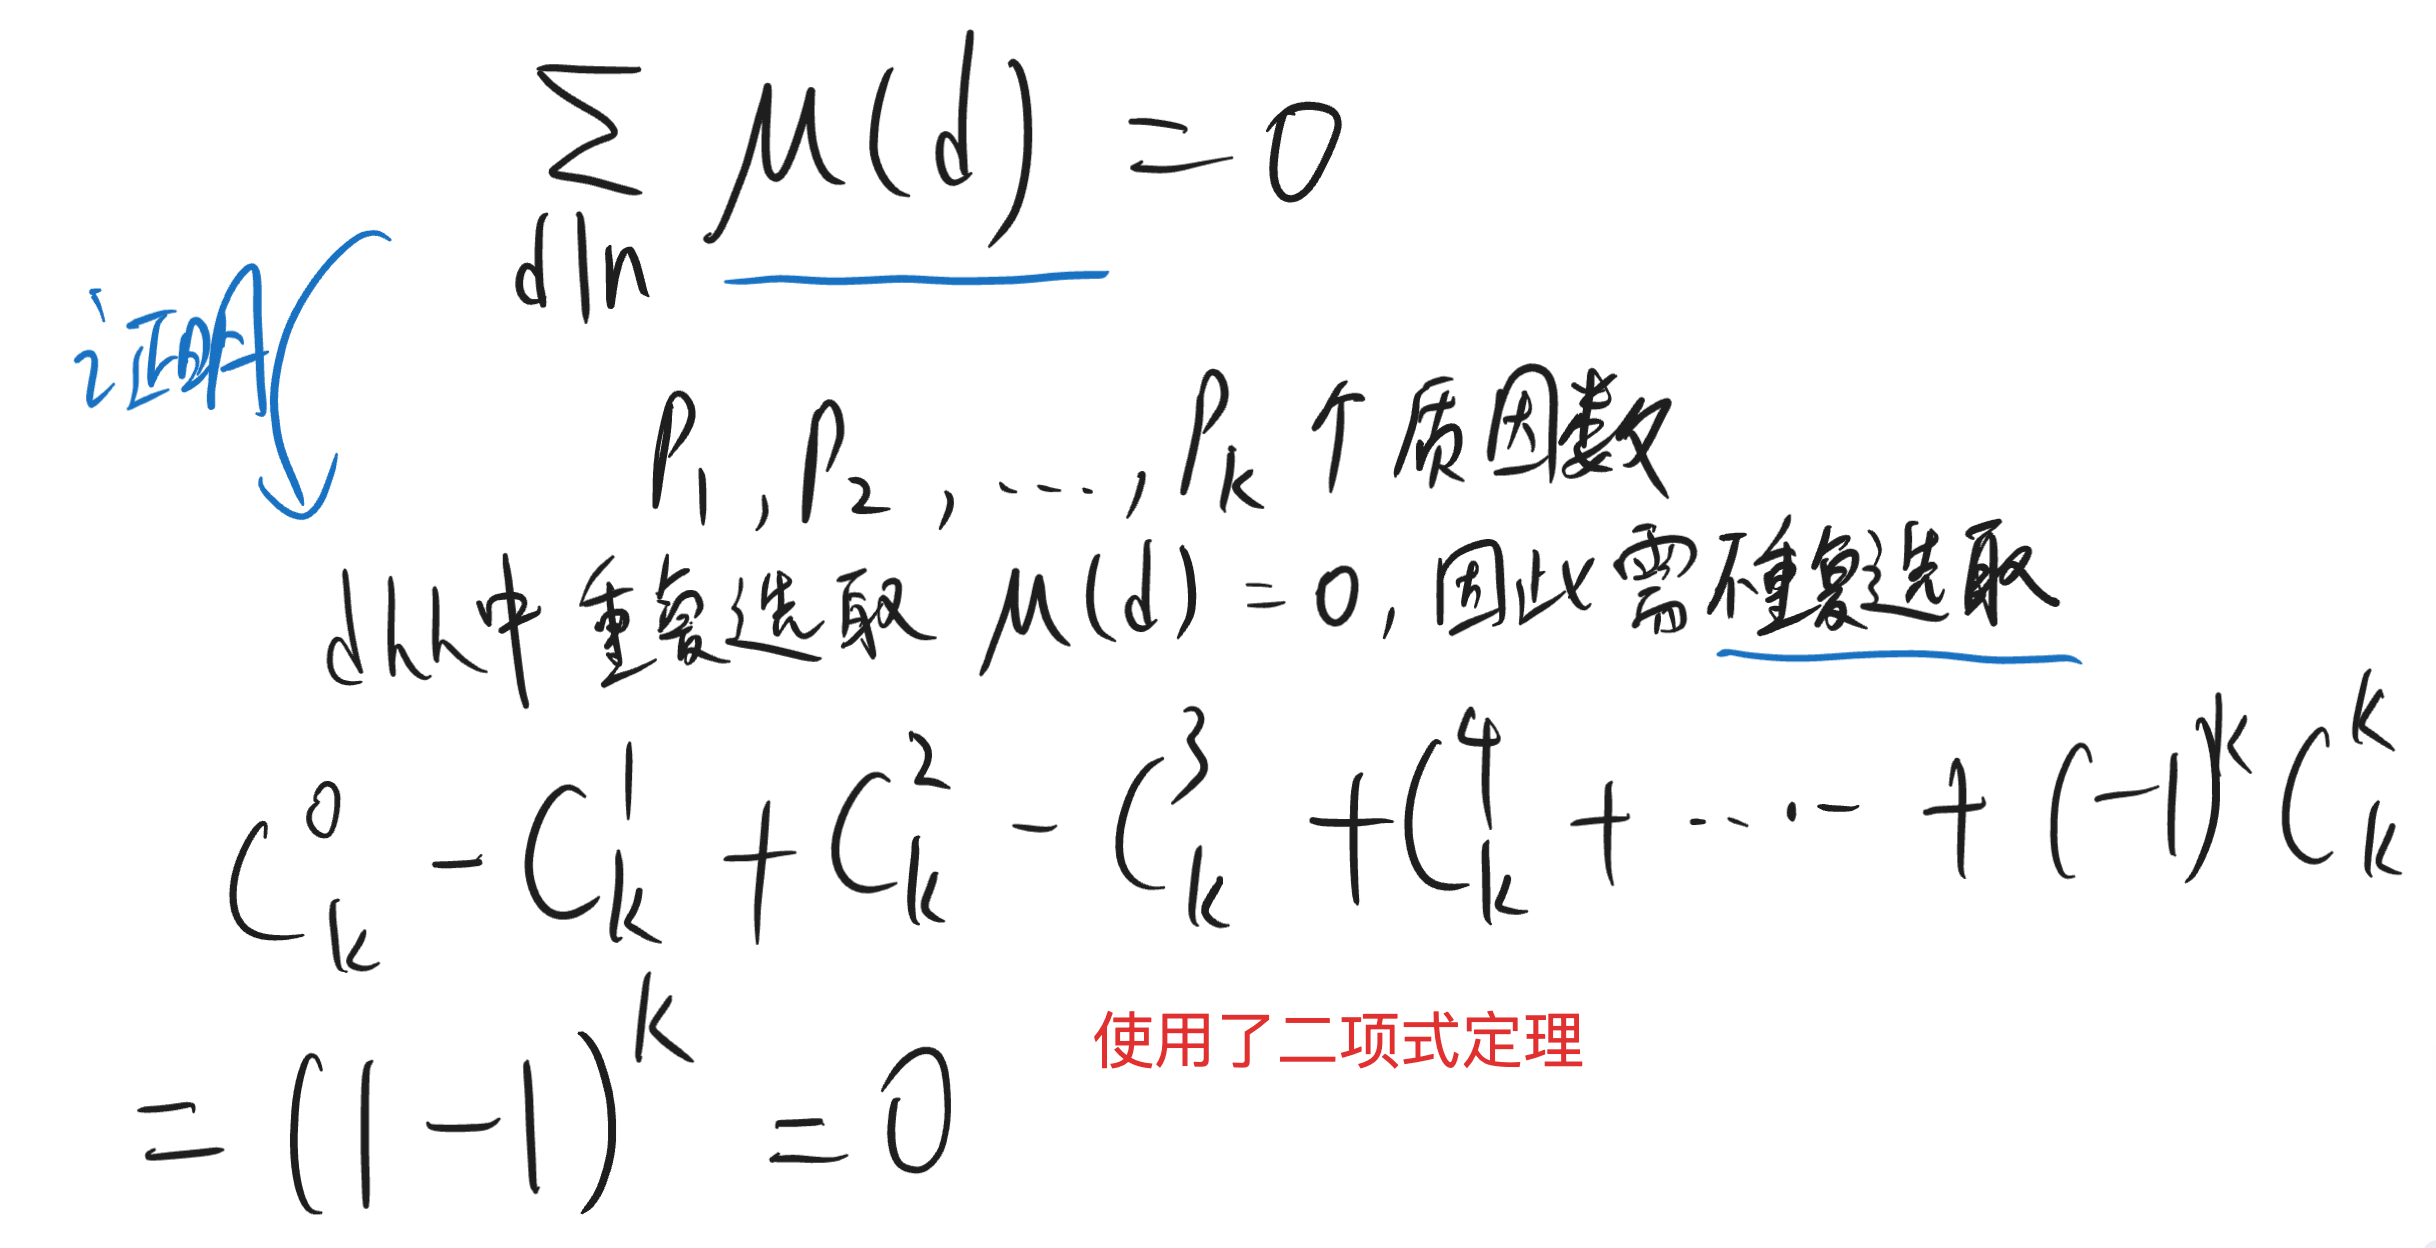
\includegraphics[width=0.92\linewidth]{image/mobius_proof_3_lemma.png}
	\end{center}

	\subsubsection{反演公式（因数形式）的证明}

	\textbf{命题.} 已知 $f(n)=\sum_{d\mid n}g(d)$，要证 $g(n)=\sum_{d\mid n}\mu(n/d)\,f(d)$：

	\begin{center}
		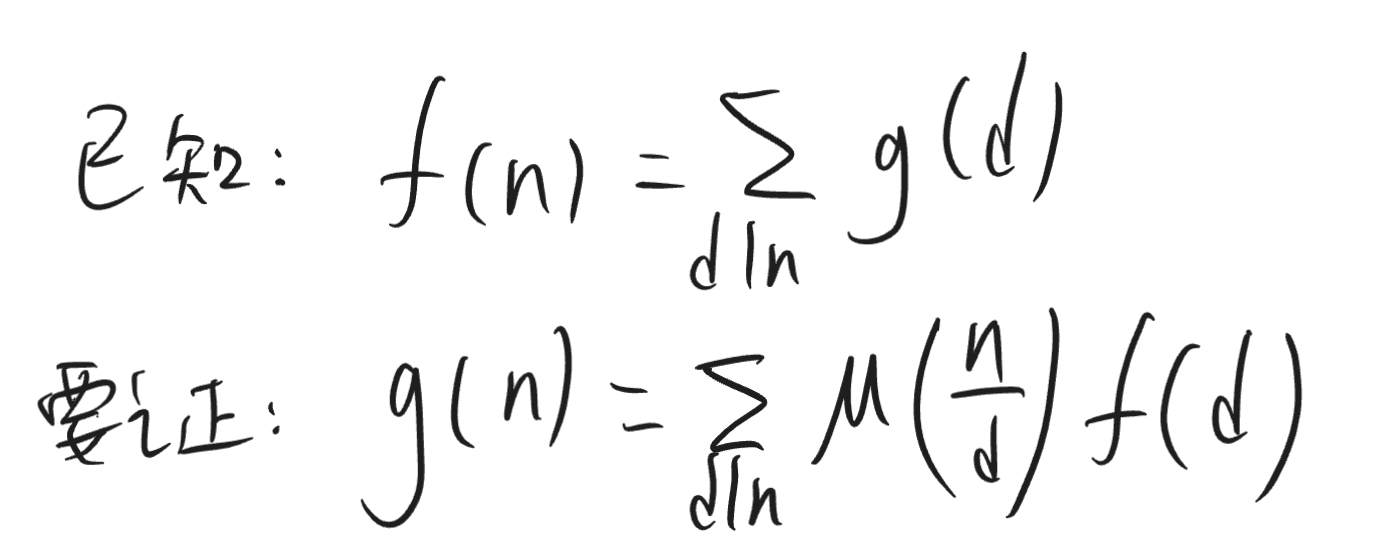
\includegraphics[width=0.72\linewidth]{image/mobius_proof_1_statement.png}
	\end{center}

	\textbf{代入并交换求和次序.} 把右边的 $f(d)$ 代入为 $\sum_{k\mid d}g(k)$，交换求和次序后令 $x=n/d$，内层中括号化为 $\sum_{x\mid n/k}\mu(x)$：

	\begin{center}
		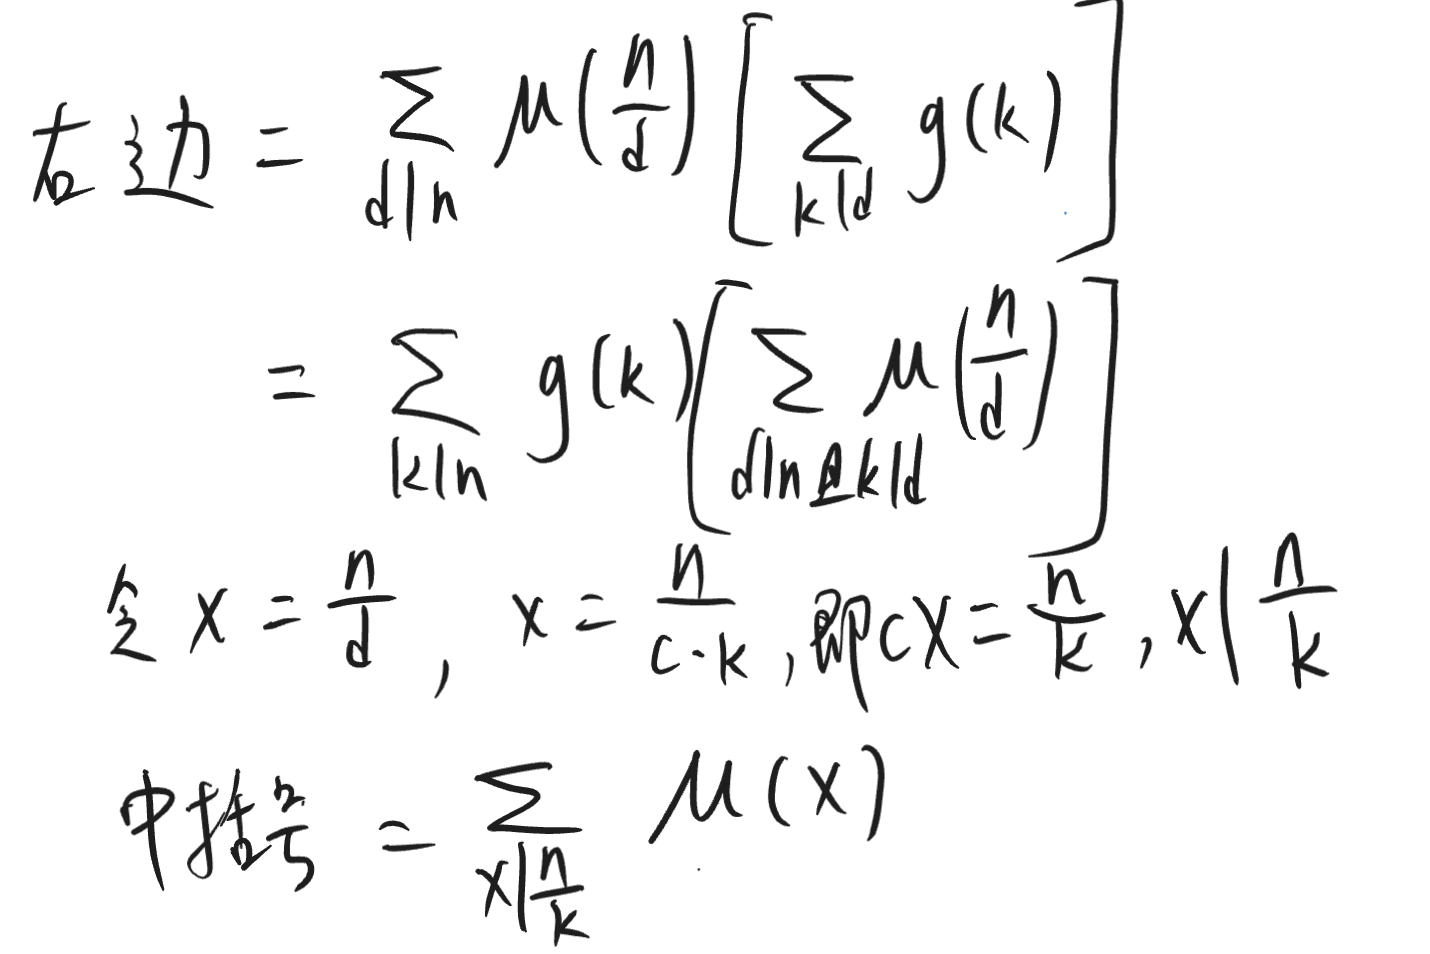
\includegraphics[width=0.80\linewidth]{image/mobius_proof_2_swap.png}
	\end{center}

	\textbf{用 $\mu$ 的性质收束.} 由关键引理 $\sum_{x\mid n/k}\mu(x)=[\,n/k=1\,]=[\,k=n\,]$，于是右边 $=\sum_{k\mid n}g(k)\,[\,k=n\,]=g(n)=$ 左边，得证：

	\begin{center}
		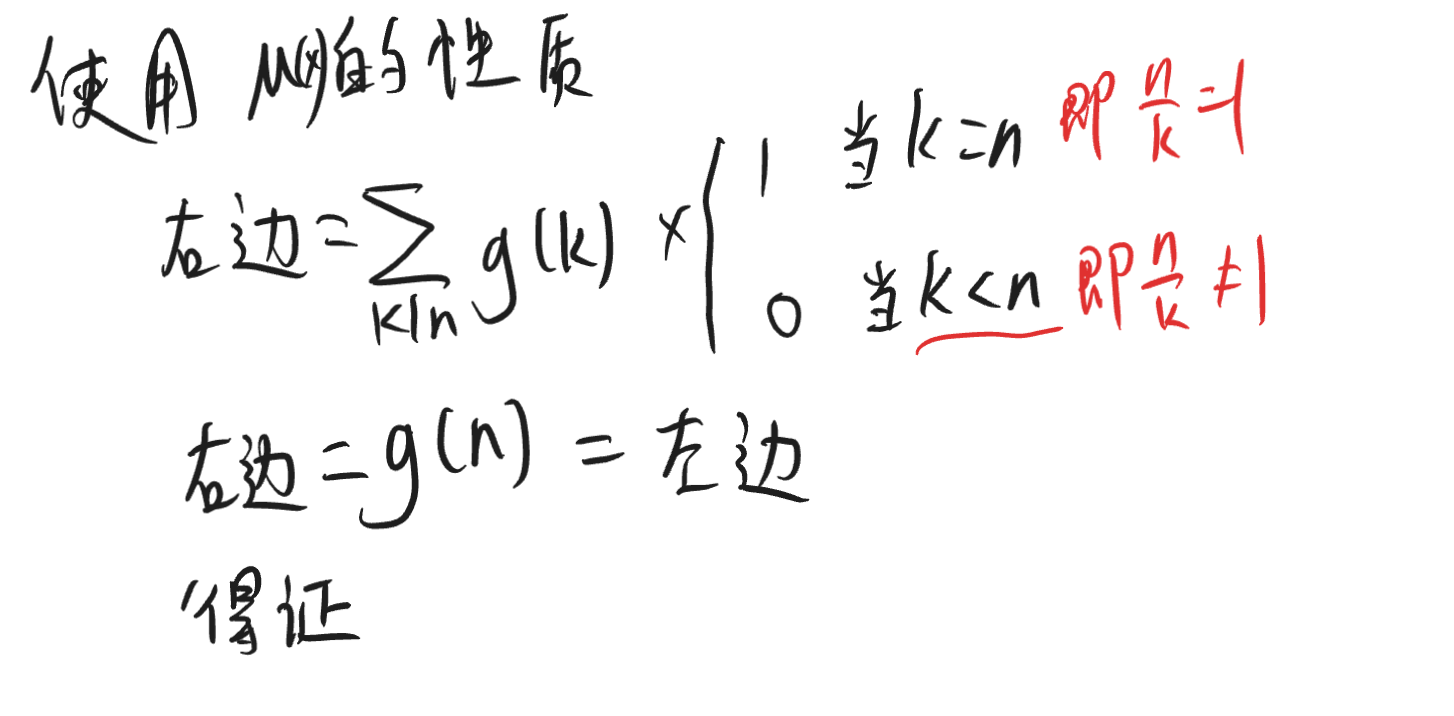
\includegraphics[width=0.82\linewidth]{image/mobius_proof_4_finish.png}
	\end{center}

	\textbf{求和次序交换示意（$n=12$）.} 上面「交换求和次序」一步，可用约数 incidence 网格直观理解——原式与交换后覆盖的是同一批 $(k,d)$ 点对：

	\begin{center}
	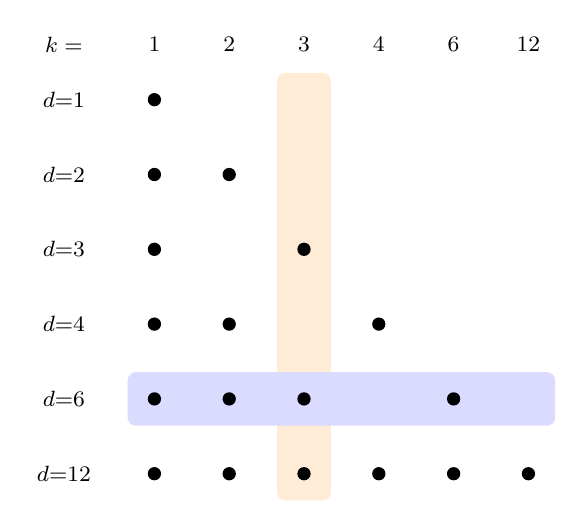
\begin{tikzpicture}[scale=1.0]
		% 12 的约数：k 作列（横轴），d 作行（纵轴，自上而下）
		% D = {1,2,3,4,6,12}，索引 0..5
		% 列高亮：k=3（第 2 列，j=2）——固定 k、纵向对 d 求和
		\fill[orange!16, rounded corners=3pt] (2*0.95-0.34, 0.34) rectangle (2*0.95+0.34, -5*0.95-0.34);
		% 行高亮：d=6（第 4 行，i=4）——固定 d、横向对 k 求和
		\fill[blue!14, rounded corners=3pt] (-0.34, -4*0.95+0.34) rectangle (5*0.95+0.34, -4*0.95-0.34);

		% 列标题 k
		\foreach \j/\kv in {0/1,1/2,2/3,3/4,4/6,5/12}
			\node[font=\footnotesize] at (\j*0.95, 0.7) {$\kv$};
		\node[font=\footnotesize] at (-1.15, 0.7) {$k=$};
		% 行标题 d
		\foreach \i/\dv in {0/1,1/2,2/3,3/4,4/6,5/12}
			\node[font=\footnotesize] at (-1.15, -\i*0.95) {$d{=}\dv$};

		% 每个 k | d 的格子画实心点（incidence）
		\foreach \i/\js in {0/{0}, 1/{0,1}, 2/{0,2}, 3/{0,1,3}, 4/{0,1,2,4}, 5/{0,1,2,3,4,5}}
			\foreach \j in \js
				\fill[black] (\j*0.95, -\i*0.95) circle (2.4pt);
	\end{tikzpicture}

	{\footnotesize 求和次序交换（$n=12$，约数 $\{1,2,3,4,6,12\}$）：实心点表示 $k \mid d$。\textcolor{blue}{蓝行}是原式「固定 $d=6$、横向对 $k \mid d$ 求和」；\textcolor{orange}{橙列}是交换后「固定 $k=3$、纵向对满足 $k \mid d \mid n$ 的 $d$ 求和」。两种方式覆盖的是同一批点，故可交换。}
	\end{center}

	\input{sections/04_count_combinatorics.tex}
	\input{sections/05_game_theory.tex}
	\input{sections/06_bitwise_identities.tex}
	\input{sections/07_basic_algorithm.tex}
	\input{sections/08_data_structure.tex}
	\input{sections/09_graph.tex}
	\input{sections/10_string_algorithm.tex}
		\begin{center}
		\section{动态规划（dp）}
	\end{center}

	\begin{multicols*}{2}

		\subsection{二进制子集枚举技巧}
		如果要枚举 $n$ 个元素的所有子集，最直接的写法是把每个集合看成一个二进制数，范围就是 $[0, 2^n - 1]$。

		\begin{minted}{cpp}
for (int s = 0; s < (1 << n); s++) {
	// s 的二进制表示对应一个子集
}
		\end{minted}

		\subsubsection{枚举某个集合的所有子集}
		如果已经有一个集合 \texttt{mask}，想要只枚举它的所有子集，常用下面这个写法。

		\begin{minted}{cpp}
for (int sub = mask; sub; sub = (sub - 1) & mask) {
	// sub 是 mask 的一个非空子集
}
		\end{minted}

		它的原理是，\texttt{sub - 1} 会把 \texttt{sub} 最低位的一个 $1$ 变成 $0$，并把它右边的若干位全部变成 $1$。随后再与 \texttt{mask} 做一次按位与，就会把不属于 \texttt{mask} 的位置全部清掉，于是得到一个更小但仍然合法的子集。

		因此，这个过程会按照从大到小的顺序，不重不漏地枚举出 \texttt{mask} 的所有非空子集。

		如果还需要处理空集，可以写成下面这样。注意 \texttt{sub == 0} 时必须及时跳出，不然会死循环。

		\begin{minted}{cpp}
for (int sub = mask;; sub = (sub - 1) & mask) {
	// sub 是 mask 的一个子集，包含空集
	if (sub == 0) {
		break;
	}
}
		\end{minted}

		这个技巧在状压 DP 中非常常见。若外层再枚举所有 \texttt{mask}，内层枚举它的全部子集，总复杂度是 $O(3^n)$。

		\subsubsection{枚举固定大小的子集}
		如果只关心恰好选了 \texttt{use} 个元素的状态，就没必要把所有状态都扫一遍再用 \texttt{popcount} 过滤。可以直接枚举二进制中恰好有 \texttt{use} 个 $1$ 的状态。

		\begin{minted}{cpp}
for (int use = 0; use <= K; ++use) {
	long long sta = (1LL << use) - 1;
	while (sta < (1LL << K)) {
		// sta 的二进制中恰好有 use 个 1

		if (sta == 0) break;  // use=0 时只对应空集这一个状态，避免下面除零
		long long c = sta & -sta;
		long long r = sta + c;
		sta = (((r ^ sta) >> 2) / c) | r;
	}
}
		\end{minted}

		这里先令 \texttt{sta = (1LL << use) - 1}，也就是二进制下最小的、恰好含有 \texttt{use} 个 $1$ 的状态。后面的转移则负责直接跳到“下一个同样有 \texttt{use} 个 $1$ 的状态”。

		\texttt{c = sta \& -sta} 会取出最低位的 $1$，\texttt{r = sta + c} 可以理解为把最靠右、还能向左移动的一位 $1$ 往前推一格。这样一来，右侧结构会被打乱，再用最后那一行把剩余的若干个 $1$ 重新挪到最右边，于是就得到了下一个更大的合法状态。

		这个写法常被称为 \texttt{Gosper's hack}。它会按照从小到大的顺序，直接跳到下一个二进制中有相同个数 $1$ 的状态。若 \texttt{use = 0}，则只对应空集这一个状态。

		\subsection{SOS DP（Sum / Max over Subsets，高维前缀和）}

		给定一个长度为 $2^N$ 的数组 $f[\,\cdot\,]$（下标看成 $N$ 位二进制掩码），希望对每个 $mask$ 求出
		$$F[mask] = \bigoplus_{sub \subseteq mask} f[sub]$$
		其中 $\bigoplus$ 可以是 $+$ / $\max$ / $\min$ / 异或等任何幺半群运算。直接枚举子集是 $O(3^N)$；SOS DP 通过\textbf{逐位扩展}把它压到 $O(N \cdot 2^N)$。

		核心思想是把每一位看成一个维度，依次做「沿第 $i$ 维的一维前缀」：当处理到第 $i$ 位时，若 $mask$ 第 $i$ 位是 $1$，就把 $mask$ 与 $mask \oplus (1 \!\ll\! i)$（去掉第 $i$ 位）合并。等价于沿 $N$ 个超立方体维度各做一遍一维前缀和。

		\textbf{对偶版}：超集而非子集，即 $F[mask] = \bigoplus_{mask \subseteq sup} f[sup]$。把转移方向反过来，把「有第 $i$ 位的从无第 $i$ 位的吸收」改成「无第 $i$ 位的从有第 $i$ 位的吸收」即可。

		\subsubsection{典型应用：按位无交最大值}

		问题：给定 $n$ 个非负整数 $a_1, \dots, a_n$，对每个 $i$ 找出最大的 $a_j$ 使得 $a_i \,\&\, a_j = 0$（按位无交集，二进制位上互不相交）。

		做法：
		\begin{itemize}
			\item 用 $dp[mask] = \max\{a_j : a_j \subseteq mask\}$（位掩码意义下的子集），初值 $dp[a_j] = a_j$。
			\item 跑一遍\textbf{子集 max}的 SOS DP，得到「掩码 $mask$ 下所有子集中最大的 $a_j$」。
			\item 对询问 $i$，答案 = $dp[\,\overline{a_i}\,]$，因为 $a_j$ 与 $a_i$ 按位无交 $\iff a_j \subseteq \overline{a_i}$。
		\end{itemize}

		复杂度 $O((V + n) \cdot \log V)$，其中 $V = \max a_i$。

		\begin{minted}{cpp}
void solve() {
	int n;
	cin >> n;
	vector<int> a(n);
	for (int &x : a) cin >> x;
	const int V = ranges::max(a);
	const int N = 32 - __builtin_clz(V); // 用到的位数
	vector<int> dp(1 << N);
	for (int x : a) dp[x] = x;           // 标记原始集合

	// SOS DP：dp[mask] = max{a_j : a_j 的位是 mask 的子集}
	for (int i = 0; i < N; i++) {
		for (int mask = (1 << N) - 1; mask >= 0; mask--) {
			if ((mask >> i) & 1) {
				dp[mask] = max(dp[mask],
				               dp[mask ^ (1 << i)]);
			}
		}
	}

	// 查询：与 a[i] 按位无交 等价于 是 ~a[i] 的子集
	for (int i = 0; i < n; i++) {
		int q = (~a[i]) & ((1 << N) - 1);
		cout << (dp[q] == 0 ? -1 : dp[q]) << " \n"[i == n - 1];
	}
}
		\end{minted}

		\textbf{要点}：
		\begin{itemize}
			\item 第二重循环\textbf{方向无关}（顺序、逆序都对），因为转移只涉及「同一 $i$ 位下，$mask$ 与去掉该位的 $mask \oplus (1 \!\ll\! i)$」，去掉位的 $mask$ 在本轮不会被本轮的更新二次覆盖（它的第 $i$ 位是 $0$，进不了 \texttt{if} 分支）。
			\item 用「0 表示未出现」的哨兵时，要确保 $a_j \neq 0$；否则要换 \texttt{-INF} 或者额外的 \texttt{exists} 标志位。
			\item 改成求\textbf{方案数}就把 \texttt{max} 换成 \texttt{+}，求\textbf{异或}就换成 \texttt{\^{}}，模板完全一致。
		\end{itemize}

		\subsection{子集格最短路（超集和 + 状压 DP 求最优排列）}

		\textbf{通用模型}：要给 $m$ 个元素定一个处理顺序（一个排列），把元素 $j$ 排在「已处理集合 $S$」之后的代价是 $\mathrm{cost}(S, j)$——注意它\textbf{只跟 $S$ 和 $j$ 有关}，跟 $S$ 内部的先后顺序无关。求总代价最小的排列。

		这类问题等价于\textbf{子集格上的最短路}：把 $2^m$ 个子集当结点，从 $S$ 向 $S \cup \{j\}$ 连一条权为 $\mathrm{cost}(S, j)$ 的边，答案就是 $\varnothing \to \{0,1,\dots,m-1\}$ 的最短路。因为边只从小集合指向大集合，图天然是 DAG，按 $mask$ 升序扫一遍就是拓扑序，不用 Dijkstra。

		\begin{center}
		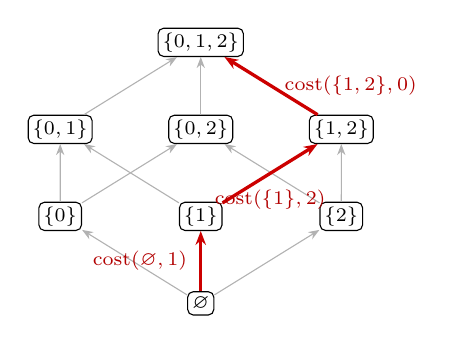
\begin{tikzpicture}[scale=0.85, every node/.style={font=\scriptsize},
			st/.style={draw, rounded corners=2pt, inner sep=1.6pt, fill=white},
			ed/.style={-{Stealth[length=4pt]}, gray!60}]
			\node[st] (e)   at (0,0)      {$\varnothing$};
			\node[st] (a0)  at (-2.1,1.3) {$\{0\}$};
			\node[st] (a1)  at (0,1.3)    {$\{1\}$};
			\node[st] (a2)  at (2.1,1.3)  {$\{2\}$};
			\node[st] (b01) at (-2.1,2.6) {$\{0,1\}$};
			\node[st] (b02) at (0,2.6)    {$\{0,2\}$};
			\node[st] (b12) at (2.1,2.6)  {$\{1,2\}$};
			\node[st] (f)   at (0,3.9)    {$\{0,1,2\}$};
			\foreach \x/\y in {e/a0, e/a2, a0/b01, a0/b02, a1/b01, a2/b02, a2/b12, b01/f, b02/f}
				\draw[ed] (\x) -- (\y);
			% 一条候选顺序：先 1，再 2，最后 0
			\draw[-{Stealth[length=5pt]}, red!80!black, very thick] (e)   -- (a1)
				node[midway, left=1pt, red!70!black] {$\mathrm{cost}(\varnothing,1)$};
			\draw[-{Stealth[length=5pt]}, red!80!black, very thick] (a1)  -- (b12)
				node[midway, below=2pt, red!70!black] {$\mathrm{cost}(\{1\},2)$};
			\draw[-{Stealth[length=5pt]}, red!80!black, very thick] (b12) -- (f)
				node[midway, right=1pt, red!70!black] {$\mathrm{cost}(\{1,2\},0)$};
		\end{tikzpicture}
		\end{center}

		图中红色一条 $\varnothing \to \{1\} \to \{1,2\} \to \{0,1,2\}$ 对应排列 $(1, 2, 0)$，路径长度就是这个排列的总代价；$m!$ 种排列被压进 $2^m$ 个结点里，这正是状压 DP 省下阶乘的地方。

		\textbf{代价怎么来}：常见形态是「每条数据带一个能力掩码 $mask$ 与一组权 $w[\,\cdot\,]$，元素 $j$ 排在 $S$ 之后要付出所有 $mask \supseteq S$ 的那些数据的 $w[j]$」。先把每条数据按 $mask$ 装桶累加，再对每一维做\textbf{超集和}（上一节 SOS DP 的对偶版），桶就原地变成了 $\mathrm{cost}(S, j)$。

		\textcolor{red!75!black}{\textbf{SOS DP 的精髓：外层先枚举维度，内层才枚举状态}}。高维前缀和 / 超集和的本质是「\textbf{对每一维各做一次}一维前缀和」，$m$ 维就是 $m$ 轮，每轮把这一维「压平」。两层循环\textbf{写反就是错的}：外层若是状态、内层是维度，同一个状态在一次内层里连着吃多个方向的超集，而那些超集已被部分更新，导致\textbf{重复计数}。$m = 2$ 的反例（记初值 $f_{00}, f_{01}, f_{10}, f_{11}$，$S$ 倒序）：

		\begin{center}
		\begin{tabular}{l|l}
			写法 & $cost[00]$ 最终值 \\ \hline
			\textcolor{red!75!black}{状态在外（错）} & $f_{00}+f_{01}+f_{10}+\textcolor{red!75!black}{2}f_{11}$ \\
			维度在外（对） & $f_{00}+f_{01}+f_{10}+f_{11}$ \\
		\end{tabular}
		\end{center}

		错的那行里 $f_{11}$ 被经 $01$ 与 $10$ 各加了一次。反过来，维度在外时\textbf{内层状态的枚举顺序无所谓}（正序倒序都对）：本轮只改第 $i$ 位为 $0$ 的状态，而被读的 $S \cup \{i\}$ 第 $i$ 位是 $1$、本轮不会被改，层内没有依赖。口诀：\textbf{维度在外，状态在内}。

		\textbf{例题}：\href{https://ac.nowcoder.com/acm/contest/133879/C}{2026 牛客多校 4 C. Retest Queue}——$n \le 2\times 10^4$ 个程序、$m \le 20$ 个测试点，测试队列可任意重排；每个程序从队首依次跑，\textbf{遇到第一个 rejected 的测试就停}（那个测试本身仍计时），程序 $i$ 跑测试 $j$ 花 $d_{i,j}$，求最小总耗时。令 $mask_i$ = 程序 $i$ 能 accept 的测试集合，把测试 $j$ 排在已排集合 $S$ 之后时，此刻\textbf{还没停下来}的程序恰是那些 $mask_i \supseteq S$ 的，它们都要付 $d_{i,j}$，于是
		$$\mathrm{cost}(S, j) = \sum_{mask_i \supseteq S} d_{i,j},$$
		正是按 $mask_i$ 装桶后的超集和。样例最优顺序 $(2,1,3)$ 的三段耗时 $10$、$1+5$、$2+2+7$ 合计 $27$。

		\textbf{复杂度}：装桶 $O(nm)$，超集和 $O(2^m m^2)$，最短路 $O(2^m m)$；空间 $2^m m$ 个 \verb|ll|（$m = 20$ 时约 $160\,\mathrm{MB}$，\verb|vector<vector<ll>>| 还要多 $2^m$ 个 vector 头约 $24\,\mathrm{MB}$——卡内存就换一维 \verb|vector<ll>| 按 $S \cdot m + j$ 行主序拍平，顺带少一层间接寻址）。

		\begin{minted}[highlightlines={33-38}, highlightcolor=red!12]{cpp}
// N 个程序, M 个测试点
// D[i][j]  = 程序 i 跑测试 j 的耗时
// masks[i] = 程序 i 能 accept 的测试集合
void Solve() {
	cin >> N >> M;
	vector<vector<ll> > D(N + 2, vector<ll>(M));
	vector<ll> masks(N + 2);
	for (int i = 1; i <= N; ++i) {
		for (int j = 0; j < M; ++j) {
			cin >> D[i][j];
		}
		ll mask = 0;
		for (int j = 0; j < M; ++j) {
			char ch;
			cin >> ch;
			if (ch == 'A') {
				mask |= 1ll << j;
			}
		}
		masks[i] = mask;
	}

	// 装桶: 把每个程序的耗时整行累加到
	// 「能力恰好等于 masks[i]」的那一行
	vector<vector<ll> > cost(1ll << M,
	                         vector<ll>(M));
	for (int i = 1; i <= N; ++i) {
		for (int j = 0; j < M; ++j) {
			cost[masks[i]][j] += D[i][j];
		}
	}

	// ===== SOS DP (超集和) =====
	// 外层 i 是「维度」, 不是状态!! 顺序写反就错
	for (int i = 0; i < M; ++i) {
		// 内层 sta 正序倒序都行: 被加的 tosta
		// 第 i 位是 1, 本层不会被改, 无层内依赖
		for (int sta = (1 << M) - 1; sta >= 0; --sta) {
			if (!((sta >> i) & 1)) {
				ll tosta = sta | (1 << i);
				for (int j = 0; j < M; ++j) {
					cost[sta][j] += cost[tosta][j];
				}
			}
		}
	}

	// 子集格最短路: mask 升序天然是拓扑序,
	// 不需要 Dijkstra
	vector<ll> Dis(1 << M, INF);
	Dis[0] = 0;
	for (int sta = 0; sta < (1 << M); ++sta) {
		for (int j = 0; j < M; ++j) {
			if (!((sta >> j) & 1)) {
				ll tosta = sta | (1 << j);
				Dis[tosta] = min(Dis[tosta],
				        Dis[sta] + cost[sta][j]);
			}
		}
	}
	cout << Dis[(1 << M) - 1] << "\n";
}
		\end{minted}

		\subsection{线段树维护 dp 求最大独立集}

		把「区间最大独立集」拍成可合并信息：每个区间维护 $dp[i][j]$，$i, j \in \{0, 1\}$ 表示该区间左端点是否选、右端点是否选时的最大权和。合并时若左区间右端 $j = 1$ 且右区间左端 $x = 1$ 则非法（相邻同选）。单点 \texttt{Info(x)}：\texttt{dp[1][1] = x}，\texttt{dp[0][0] = 0}，对角 $-\infty$。区间查询直接 \texttt{seg.query(l, r)} 得到该段最大独立集（四个状态取 max）。

		参考提交：\href{https://atcoder.jp/contests/abc456/submissions/75466400}{ABC 456 提交 75466400}。

		\begin{minted}{cpp}
struct Info {
  array<array<ll, 2>, 2> dp;
  Info(ll x = 0) {
    dp[0][1] = dp[1][0] = -INF;
    dp[1][1] = x;
    dp[0][0] = 0;
  }
};

Info operator+(const Info &a, const Info &b) {
  Info fa;
  for (int i = 0; i <= 1; i++) {
    for (int j = 0; j <= 1; j++) {
      if (a.dp[i][j] == -INF) continue;
      for (int x = 0; x <= 1; x++) {
        for (int y = 0; y <= 1; y++) {
          if (b.dp[x][y] == -INF) continue;
          if (j == 1 && x == 1) continue;
          fa.dp[i][y] = max(a.dp[i][j] + b.dp[x][y], fa.dp[i][y]);
        }
      }
    }
  }
  return fa;
}

template <class InfoType = Info>
class LazySegmentTree {
  int n;
  vector<InfoType> tree;

  void pushUp(int id) {
    tree[id] = tree[id << 1] + tree[id << 1 | 1];
  }

  void build(int id, int l, int r, const vector<InfoType> &a) {
    if (l == r) { tree[id] = a[l]; return; }
    int mid = (l + r) >> 1;
    build(id << 1, l, mid, a);
    build(id << 1 | 1, mid + 1, r, a);
    pushUp(id);
  }

  InfoType query(int id, int l, int r, int ql, int qr) {
    if (ql <= l && r <= qr) return tree[id];
    int mid = (l + r) >> 1;
    if (qr <= mid) return query(id << 1, l, mid, ql, qr);
    if (ql > mid)  return query(id << 1 | 1, mid + 1, r, ql, qr);
    return query(id << 1, l, mid, ql, qr) +
           query(id << 1 | 1, mid + 1, r, ql, qr);
  }

public:
  LazySegmentTree(int n = 0) { init(n); }
  LazySegmentTree(const vector<InfoType> &a) { build(a); }

  void init(int n_) {
    n = n_;
    tree.assign(4 * n + 5, InfoType());
  }

  void build(const vector<InfoType> &a) {
    init((int)a.size() - 1);
    if (n > 0) build(1, 1, n, a);
  }

  InfoType query(int l, int r) {
    if (l > r) return 0;
    return query(1, 1, n, l, r);
  }
};

void solve() {
  int n, k;
  cin >> n >> k;
  vector<ll> a(n + 1);
  for (int i = 1; i <= n; i++) cin >> a[i];
  vector<Info> b(n + 1);
  for (int i = 1; i <= n; i++) b[i] = Info(a[i]);
  for (int i = 1; i <= n; i++) a[i] = a[i] + a[i - 1];
  LazySegmentTree<Info> seg;
  seg.build(b);
  ll ans = INF;
  for (int len = k - 1; len <= k; len++) {
    for (int l = 1; l + len <= n; l++) {
      int r = l + len;
      ll candidate = a[r] - a[l - 1];
      auto info = seg.query(l + 1, r - 1);
      ll maxi = -INF;
      for (int i = 0; i <= 1; i++)
        for (int j = 0; j <= 1; j++)
          maxi = max(maxi, info.dp[i][j]);
      candidate -= maxi;
      ans = min(ans, candidate);
    }
  }
  cout << ans << "\n";
}
		\end{minted}

	\end{multicols*}


	\input{sections/12_geometry.tex}
		\begin{center}
		\section{STL 及其使用}
	\end{center}

	\begin{multicols*}{2}

		\subsection{\texttt{string::find} 的起始位置参数与 \texttt{string\_view}}
		\texttt{find} 可以指定「从哪个下标开始找」，但不能直接指定「查找到哪个下标结束」。

		\begin{minted}{cpp}
string s = "abacaba";
string t = "aba";

size_t pos = s.find(t, 2); // 从下标 2 开始找
if (pos == string::npos) { // string::npos 就是 -1
	// 没找到
}
		\end{minted}

		如果要限制在区间 \verb|[l, r]| 内查找，可以先从 \verb|l| 开始找，再判断匹配是否完整落在区间内（\verb|std::string_view| 是在 \verb|C++ 17| 引入的）。

		\begin{minted}{cpp}
string_view sv = s;
auto sub = sv.substr(l, r - l + 1); // 只看 [l, r]
size_t p = sub.find(t);
if (p != string::npos) {
	size_t real_pos = l + p; // 映射回原串下标
}
		\end{minted}

		\subsection{\texttt{mt19937\_64} 套 \texttt{splitmix64} 抗 BM 攻击}

		\begin{minted}{cpp}
std::mt19937_64 rng(std::chrono::steady_clock::now().time_since_epoch().count());

// 把 rng() 输出再过一层非线性混合，挡住 F2 上的 Berlekamp–Massey 攻击
uint64_t splitmix64(uint64_t x) {
	x ^= x >> 30; x *= 0xbf58476d1ce4e5b9ULL;
	x ^= x >> 27; x *= 0x94d049bb133111ebULL;
	return x ^ (x >> 31);
}
uint64_t rnd() { return splitmix64(rng()); } // XOR hashing 等场景用这个，别用裸 rng()
		\end{minted}

		\textbf{攻击模型出处}：\href{https://codeforces.com/blog/entry/153335}{\textit{Hacking Incorrect XOR Hashing with \texttt{mt19937\_64}}}（Sugar\_fan，CF blog）。\texttt{mt19937\_64} 的 \texttt{XOR}、移位、稀疏 $\mathbb{F}_2$ 矩阵乘全部在 $\mathbb{F}_2$ 上线性，Berlekamp–Massey 拿前 $2 \times 19937$ 个输出位即可复盘最小多项式、预测后续输出，构造 \texttt{XOR} 多重集 hash 碰撞。换种子、加 \texttt{seed\_seq}、混 \texttt{random\_device} 全无效——线性结构和种子无关。

		\textbf{\texttt{splitmix64} 包装够不够}：本地 Apple M5 + GCC 15.2 上的 benchmark（\href{https://gist.github.com/znzryb/a867eefeb8575e1c5f599a5044273614}{gist}）实证——裸 \texttt{mt19937\_64} 上 BM 在 5 个 bit lane 一致复盘出 \texttt{degree = 19937}、命中率 $100\%$；套上 \texttt{splitmix64} 后 BM 度数饱和到训练长度的一半、命中率锁在 $50\%$（bit 要么 0，要么 1，基本就是闭眼瞎猜），攻击失效。

		\subsection{\texttt{unordered\_map} 自定义 hash \& 结构体做 key}

		\textbf{为何要自定义}：GCC 整数默认 hash 是恒等（\texttt{hash<ll>(x) == x}）、桶数又走内部写死的质数序列，二者都可离线预测。攻击者构造大量落同一桶的 key，让查询退化 $O(n)$、整体 $O(n^2)$ TLE。防御 = 每次运行播一个 \texttt{static} 随机盐、混进 key 再过 \texttt{splitmix64} 打散（复用上一节的 \texttt{splitmix64}）：

		\begin{minted}{cpp}
struct custom_hash {
	size_t operator()(uint64_t x) const {
		static const uint64_t R =
			chrono::steady_clock::now().time_since_epoch().count();
		return splitmix64(x + R); // 盐 + avalanche
	}
};
// 用 alias 一键注入, 声明处跟原生一样
template <class K, class V>
using hash_map = unordered_map<K, V, custom_hash>;
hash_map<ll, int> mp;
		\end{minted}

		\textbf{自定义结构体做 key} 需要两样东西：(1) 一个 hash 把\textbf{每个字段逐个混入}（禁止直接异或，\texttt{(a,b)} 与 \texttt{(b,a)} 会撞成同值）；(2) \texttt{operator==} 供哈希冲突时比较。两个 \texttt{operator} \textbf{都要加 \texttt{const}}，否则 \texttt{unordered\_map} 对 const key 调用时编译不过：

		\begin{minted}{cpp}
struct Point {
	ll x, y;
	bool operator==(const Point &o) const { // ← const
		return x == o.x && y == o.y;
	}
};
struct PointHash {
	size_t operator()(const Point &p) const { // ← const
		static const uint64_t R =
			chrono::steady_clock::now().time_since_epoch().count();
		uint64_t h = splitmix64(p.x + R);
		return splitmix64(p.y + h); // 逐字段混, 顺序敏感
	}
};
unordered_map<Point, int, PointHash> mp;
		\end{minted}

		\textbf{坑}：\texttt{mp.reserve(n)} / \texttt{max\_load\_factor(0.25)} 只是把桶数顶大 / 保持稀疏，桶数\textbf{仍然可预测}——是弱防御 + 常数优化，\textbf{不能单独防 hack}，真正的防线永远是随机盐。追求速度可换 \texttt{\_\_gnu\_pbds::gp\_hash\_table<K, V, custom\_hash>}（开放寻址，常数更小），\texttt{custom\_hash} 用法相同。

		\subsection{\texttt{sort + unique} 按 key 去重并保留指定值}

		\texttt{std::unique} 把相邻相等元素合并为一个，\textbf{保留每段的第一个}（不是最后）。配合 \texttt{sort} 可以做「按某个 key 分组、每组只留一个特定属性最大 / 最小的元素」。

		\textbf{标准套路}：(1) 主 key 升序排（保证同 key 元素挤在一起）；(2) 次 key \textbf{反向}排，让"想留的"挤到每组最前面；(3) \texttt{unique} 用主 key 比较器去重，留下每组第一个。

		\textbf{例（\href{https://www.luogu.com.cn/problem/P3194}{洛谷 P3194} 上半包络题 dedupe 步骤）}：直线 $y = A_i x + B_i$，同斜率 $A$ 多条只留 $B$ 最大那条（其余被同斜率平行压死，对偶点全部出现在上凸壳「同 $x$ 不同 $y$ 竖边」上 strict 也救不了）。

		\begin{minted}{cpp}
sort(poly.begin(), poly.end(), [](const Point<ll> &a, const Point<ll> &b) {
	if (a.x != b.x) return a.x < b.x; // 主 key 升序
	return a.y > b.y;                 // 次 key 降序: 想留的 (B 大) 在前
});
poly.erase(unique(poly.begin(), poly.end(), [](const Point<ll> &a, const Point<ll> &b) {
	return a.x == b.x;                // 比较器只看主 key, 不看次 key
}), poly.end());
		\end{minted}

		\textbf{坑}：次 key 写反成 \texttt{a.y < b.y}（升序），\texttt{unique} 留下的是每组 B \textbf{最小}那条——和题意完全相反，是高频低级错误。\textbf{记忆口诀}：「\texttt{unique} 留前 $\to$ 想留谁就 \texttt{sort} 把谁放最前」。

		\subsection{\texttt{lower\_bound} / \texttt{upper\_bound} 自定义比较器参数顺序相反}

		\textbf{先厘清概念}：\texttt{lower\_bound} / \texttt{upper\_bound} 的第三个参数是\textbf{待查找的值}（拿来和元素的排序键比较的目标值），\textbf{不是下标 / 位置}；返回的迭代器才是「位置」。即\textbf{输入一个值，输出一个位置}。下例数组 \texttt{es} 按 \texttt{node::val} 升序排好，\texttt{target} 是要找的目标值，\texttt{e.val} 是元素的排序键字段（也是个值，不是下标）。

		带自定义比较器时，\texttt{lower\_bound} 与 \texttt{upper\_bound} 的比较器两个参数\textbf{谁前谁后是相反的}——标准强制，记反轻则二分边界静默错、重则编译不过：

		\begin{itemize}
			\item \texttt{lower\_bound(first, last, target, comp)} 内部按 \texttt{comp(*it, target)} 调用——\textbf{数组元素在前，目标值在后}，返回首个满足 \texttt{e.val} $\ge$ \texttt{target} 的位置。
			\item \texttt{upper\_bound(first, last, target, comp)} 内部按 \texttt{comp(target, *it)} 调用——\textbf{目标值在前，数组元素在后}，返回首个满足 \texttt{e.val} $>$ \texttt{target} 的位置。
		\end{itemize}

		\textbf{场景 A —— 找第一个 \texttt{e.val} $\ge$ \texttt{target} 的元素}，用 \texttt{lower\_bound}：

		\begin{minted}{cpp}
auto it = lower_bound(es.begin(), es.end(), target,
	[](const node &e, int t) {   // 元素 node 在前, 目标值 int 在后
		return e.val < t;
	});
		\end{minted}

		\textbf{场景 B —— 找第一个 \texttt{e.val} $>$ \texttt{target} 的元素}，用 \texttt{upper\_bound}：

		\begin{minted}{cpp}
auto it = upper_bound(es.begin(), es.end(), target,
	[](int t, const node &e) {   // 目标值 int 在前, 元素 node 在后
		return t < e.val;
	});
		\end{minted}

		\textbf{坑（编译错 vs 静默逻辑错）}：比较器喂错函数的后果取决于\textbf{元素类型与目标值类型是否同构}。本例元素是 \texttt{node}、目标值是 \texttt{int}，二者\textbf{异构且不可互转}：把场景 B 的 \texttt{(int, node)} 比较器误传给 \texttt{lower\_bound}，它要按 \texttt{comp(node, int)} 调，参数对不上又无 \texttt{node}/\texttt{int} 转换，\textbf{直接编译失败}。但若元素与目标值\textbf{同类型}（如拿 \texttt{node} 二分 \texttt{node}），顺序写反\textbf{能编译通过，却是静默错的二分边界}——更难查。

		\textbf{记忆口诀}：「\texttt{lower} 找 $\ge$，元素在前；\texttt{upper} 找 $>$，目标在前」。

		\subsection{\texttt{\_\_int128} 读入输出（重载运算符版）}

		\texttt{iostream} 原生不支持 \texttt{\_\_int128}。重载 \texttt{<<} / \texttt{>>} 后，\texttt{cin} / \texttt{cout} 就能像内建整型一样直接读写（也自动覆盖 \texttt{Point<i128>} 等模板类里转发的 \texttt{>>} / \texttt{<<}）：

		\begin{minted}{cpp}
ostream &operator<<(ostream &os, __int128 x) {
	if (x < 0) os << '-', x = -x;
	if (x > 9) os << x / 10;
	return os << (char) ('0' + x % 10);
}

istream &operator>>(istream &is, __int128 &x) {
	string s;
	if (!(is >> s)) return is;
	x = 0;
	size_t i = 0;
	bool neg = false;
	if (s[0] == '-') {
		neg = true;
		i = 1;
	} else if (s[0] == '+') { i = 1; }
	for (; i < s.size(); ++i) x = x * 10 + (s[i] - '0');
	if (neg) x = -x;
	return is;
}
		\end{minted}

		输出走递归除 $10$（深度 $\le 39$ 层，无爆栈风险）；读入按字符串整体读进来再逐位累加，支持前导 \texttt{-} / \texttt{+}。

		\textbf{读入开头 \texttt{if (!(is >> s)) return is;} 的用意}：让 \texttt{while (cin >> v)} 「多组输入读到 EOF 自动停」的写法对 \texttt{\_\_int128} 同样成立。\texttt{is >> s} 返回流本身，流可以转 \texttt{bool}（语义是「上一次读取成功与否」）：EOF 时读不到内容、流被置上失败位、转出 \texttt{false}，这行就直接带着失败位原样返回且\textbf{不动} \texttt{x}——与内建整型 \texttt{cin >> n} 读失败的行为对齐，外层循环条件拿到 \texttt{false} 正确退出。

		\textbf{坑}：输出对负数先 \texttt{x = -x}，恰为 $-2^{127}$（\texttt{\_\_int128} 最小值）时取负溢出是 UB——竞赛值域顶到 $\pm 1.7 \times 10^{38}$ 边界才会踩，正常使用不受影响。

		\subsection{\texttt{next\_permutation} 枚举全排列}

		\texttt{next\_permutation(first, last)} 把区间 $[\texttt{first}, \texttt{last})$ 原地重排成\textbf{字典序的下一个排列}并返回 \texttt{true}；当前已是最大排列（完全降序）时返回 \texttt{false}，并把区间重排回最小排列（完全升序）。标准套路——\textbf{先 \texttt{sort} 到最小排列，再 \texttt{do-while}}：

		\begin{minted}{cpp}
vector<int> p = {3, 1, 2};
sort(p.begin(), p.end());  // 必须从最小排列出发, 否则枚举不全
do {
	// 处理当前排列 p (do-while 保证初始排列本身也被处理)
} while (next_permutation(p.begin(), p.end()));
		\end{minted}

		\begin{itemize}
			\item \textbf{不 \texttt{sort} 就 \texttt{do-while} 是高频错误}：只会从当前排列往字典序后面枚举，前面的排列全部漏掉。
			\item \textbf{复杂度}：单次调用均摊 $O(1)$（最坏 $O(n)$），枚举全部共 $n!$ 个——$n = 10$ 约 $3.6 \times 10^6$ 随便跑，$n = 11$ 约 $4 \times 10^7$ 是边界，$n \ge 12$ 基本不可行。
			\item \textbf{有重复元素时自动去重}：按「不同的排列」恰好各枚举一次（如 \texttt{\{1, 1, 2\}} 只出 3 种），这是它比手写 DFS 全排列省心的地方。
			\item \textbf{枚举组合的技巧}：开一个 $n - k$ 个 \texttt{0} + $k$ 个 \texttt{1} 的 01 数组，\texttt{sort} 后用同一套 \texttt{do-while} 枚举它的全部排列，就是 $\binom{n}{k}$ 个组合的指示向量。
			\item 对称版本 \texttt{prev\_permutation}：字典序上一个，完全升序时返回 \texttt{false}；\texttt{string} / 数组 / \texttt{vector} 都能用（任何双向迭代器区间）。
		\end{itemize}
	\end{multicols*}


	\input{sections/14_common_pitfalls.tex}
	\input{sections/15_debug_tricks.tex}
		\begin{center}
		\section{环境测试}
	\end{center}

\begin{multicols*}{2}

	\subsection{试机赛与纪律}

	\begin{itemize}
		\item 检查身份证件：护照、学生证、胸牌以及现场所需通行证。
		\item 确认什么东西能带进场。特别注意：智能手表、金属（钥匙）等等。
		\item 测试鼠标、键盘、显示器和座椅。如果有问题，立刻联系工作人员。
		\item 测试比赛提交方式。如果有 \texttt{submit} 命令，确认如何使用。
		\item 设置自动保存、自动备份。
	\end{itemize}

	\subsection{编译器版本与扩展头}

	测试编译器版本。C++20 \verb|cin >> (s + 1)|；C++17 \verb|auto [x, y] : a|；C++14 \verb|[](auto x, auto y)|；C++11 \verb|auto|；\texttt{bits/stdc++.h}；\texttt{pb\_ds}。

	\begin{minted}{cpp}
#include <ext/rope>
using namespace __gnu_cxx;
rope<int> R; R.insert(y, x); R[x]; R.erase(x, 1);

#include <ext/pb_ds/assoc_container.hpp>
#include <ext/pb_ds/tree_policy.hpp>
using namespace __gnu_pbds;
tree<int, null_type, less<int>, rb_tree_tag,
     tree_order_statistics_node_update> s;
s.insert(1); s.find_by_order(0); s.order_of_key(5);
	\end{minted}

	\subsection{\texttt{\_\_int128}, \texttt{\_\_float128}, \texttt{long double} 实测}

	\textcolor{blue}{\textbf{long double 不是跨平台稳定类型}}：在 \textcolor{blue}{\textbf{x86-64 Linux + GCC}}（CF / AtCoder / QOJ 评测机）上是 80-bit x87 扩展精度（尾数 64 bits、约 18--19 位有效、\texttt{LDBL\_EPSILON} $\approx 1.08 \times 10^{-19}$），但 \textcolor{blue}{\textbf{Apple arm64 / MSVC}} 上 \texttt{long double == double}（尾数 53 bits、约 15 位、$\epsilon \approx 2.22 \times 10^{-16}$）。本机过 $\not\Rightarrow$ 评测机过。

%	\textcolor{blue}{\textbf{评测机看不到 stdout，必须用 \texttt{assert} 把判定接到 verdict 上}}：AC = 条件成立、RE = 条件不成立、CE = 类型 / 头文件不可用。开赛随便挑一道签到题，把下面塞进 \texttt{main} 顶部提交：

	\begin{minted}{cpp}
#include <bits/stdc++.h>
// pb_ds / rope 是否可用：能编过即 OK
#include <ext/pb_ds/assoc_container.hpp>
#include <ext/rope>

// long double 是不是真扩展精度（CE = 退化成 double 或编译器异常）
static_assert(sizeof(long double) > sizeof(double), "ld == double");
static_assert(LDBL_MANT_DIG >= 64, "ld mantissa < 64 bits");

int main() {
    std::cout << "sizeof(long double)=" << sizeof(long double) << '\n';
    std::cout << "LDBL_MANT_DIG=" << LDBL_MANT_DIG << '\n';
    // QOJ x86-64 Linux 实测 sizeof=16 (10B 80-bit 数据 + 6B 对齐 padding), mant=64
    // 相对精度 LDBL_EPSILON ~ 2^-63 ~ 1.08e-19（vs double 2.22e-16，多 ~3 位有效数字）
    // __int128 是否可用（不可用直接 CE）。assert 必须在函数体内，namespace scope 不合法
    __int128 x = (__int128)1 << 100; assert(x > 0);
    // __float128 是否可用（GCC 扩展，MSVC 无；不可用 CE）
    // 1.0Q 字面量需 -fext-numeric-literals 才认；用 cast 跨编译选项更稳
    __float128 y = (__float128)1; assert(y == 1);
}
	\end{minted}

	注意 \texttt{\_\_int128} 的 \texttt{cin/cout} 不支持，需手写 read/print；\texttt{\_\_float128} 是软件模拟，慢一档。重载 \texttt{operator<<} / \texttt{operator>>} 后 \texttt{cin >> x} / \texttt{cout << x} 即可直接吃 \texttt{\_\_int128}：

	\begin{minted}{cpp}
ostream &operator<<(ostream &os, __int128 x) {
    if (x < 0) os << '-', x = -x;
    if (x > 9) os << x / 10;
    return os << (char) ('0' + x % 10);
}

istream &operator>>(istream &is, __int128 &x) {
    string s;
    if (!(is >> s)) return is;
    x = 0;
    size_t i = 0;
    bool neg = false;
    if (s[0] == '-') {
        neg = true;
        i = 1;
    } else if (s[0] == '+') { i = 1; }
    for (; i < s.size(); ++i) x = x * 10 + (s[i] - '0');
    if (neg) x = -x;
    return is;
}
	\end{minted}

	\subsection{评测机限制与编译选项}

	\begin{itemize}
		\item 测试代码长度限制，尝试触发 \texttt{NO-OUTPUT}、\texttt{OUTPUT-LIMIT}、\texttt{RUN-ERROR}。
		\item 测试 \verb|#pragma GCC optimize| / \verb|#pragma GCC target| 是否会被判为 CE（本机自带一半答案，详见下面「\texttt{\#pragma} 开优化 / SIMD 实测」一节）。
		\item 测试 clarification：如果问不同类型的愚蠢问题，得到的回复是否不一样？
		\item 测试 \verb|-fsanitize=address|、\verb|-fsanitize=undefined|、\verb|-D_GLIBCXX_DEBUG| 是否可用。
		\item 测试 \verb|/usr/bin/time -v ./a.out| 是否能显示内存占用。
	\end{itemize}

	\subsection{\texttt{\#pragma} 开优化 / SIMD 实测}

	开 O3 三条路径，可叠加；\textcolor{blue}{\textbf{源码 pragma 优先级高于命令行}}（同 TU 内覆盖 \texttt{-O} flag）。

	\begin{minted}{cpp}
// 命令行：本机训练默认；-march=native 评测机别带
// g++ -O3 -std=c++20 a.cpp

// optimize 放 include 之前；target 必须放 include 之后（见下方踩坑 d）
#pragma GCC optimize("O3,unroll-loops")
#include <bits/stdc++.h>
#ifdef __x86_64__
#pragma GCC target("avx2,bmi,bmi2")
#endif
int main() { std::vector<int> v(5); v[0] = 1; }  // 自检要触发 STL 实例化
	\end{minted}

	实测（$N = 2^{20}$ 浮点 mul-add 200 轮，5 次中位数）：

	\begin{center}
		\small
		\begin{tabular}{l|l}
			\hline
			编译方式                                 & 时间      \\
			\hline
			\texttt{-O2}（评测机默认）               & $120$ ms  \\
			\texttt{-O3}                              & $117$ ms  \\
			\texttt{-O3 -funroll-loops}               & $113$ ms  \\
			\texttt{\#pragma optimize("O3,unroll-loops")} & $114$ ms  \\
			\hline
		\end{tabular}
	\end{center}

	评测机默认 \texttt{-O2}，所以 \texttt{\#pragma optimize("O3")} 的实际收益是 \textbf{O3 比 O2 快约 3\%、加 \texttt{unroll-loops} 共约 6\%}——不是"几倍加速"。其更主要价值是兜底：评测机若被设成 \texttt{-O0/-O1}（少见但确实有），pragma 自动把模板抬回 O3。

	\textbf{踩坑}：(a) \texttt{target("avx2")} 在 arm64 硬 CE，模板里此类代码段默认假设 x86 评测机。(b) pragma 路径下 \texttt{\_\_OPTIMIZE\_\_} 不定义（后端才 apply），不能拿来自检。(c) Mac 系统 \texttt{g++} 是 clang shim、不认这套 pragma 也找不到 \texttt{bits/stdc++.h}，本地必须显式调 \texttt{g++-15}。(d) \textcolor{blue}{\textbf{\texttt{\#pragma GCC target} 必须放在 \texttt{\#include <bits/stdc++.h>} 之后}}：放之前会让 libstdc++ 头里 \texttt{always\_inline} 模板（如 \texttt{\textasciitilde{}allocator} / \texttt{\_Vector\_impl}）带上 SIMD target，CF 用的 winlibs MinGW GCC 上 user 代码用 \texttt{vector<>} 等触发 inline 时报 \texttt{target specific option mismatch} CE（Linux GCC 不触发）。

	\textbf{评测机自检}：把上段提交到任意评测机——CE 就是 pragma 被拒，AC 就是 pragma 全收。\textbf{自检源码必须实例化 STL}（如 \texttt{vector<int> v(5)}），空 \texttt{main} 不触发模板 inline、是假绿灯。

	\subsection{性能基准（map 跑分）}

	跑分覆盖 \textcolor{blue}{\textbf{STL 容器 + 随机访存 + 比较器内联}}这套 CP 真实热点。\texttt{std::map} 的插入查找把红黑树指针追逐 + L2/L3 miss + \texttt{operator<} 内联效果都能压出来。计时用 \texttt{chrono::steady\_clock}（wall-clock，纳秒分辨率，跨平台语义一致）而不是 \texttt{clock()}（Windows MSVC 上是 wall-clock、Linux glibc 上是 CPU 时间，跨评测机数字没法直接比）。标定 \texttt{1s} 能跑多少次：

	\begin{minted}{cpp}
#include <bits/stdc++.h>
using namespace std;

// 文件作用域：高精度 steady_clock 种子 + splitmix64 非线性混合（同 §10.4）
mt19937_64 rng(chrono::steady_clock::now().time_since_epoch().count());
uint64_t splitmix64(uint64_t x) {
    x ^= x >> 30; x *= 0xbf58476d1ce4e5b9ULL;
    x ^= x >> 27; x *= 0x94d049bb133111ebULL;
    return x ^ (x >> 31);
}

int main() {
    const int N = 1 << 20;
    vector<uint64_t> keys(N);
    for (int i = 0; i < N; i++) keys[i] = splitmix64(rng());
    auto t0 = chrono::steady_clock::now();
    map<uint64_t, int> mp;
    for (int i = 0; i < N; i++) mp[keys[i]] = i;          // 插入
    long long s = 0;
    for (int i = 0; i < N; i++) s += mp[keys[i]];         // 查找
    assert(s != 0);                                        // 防 DCE + 弱正确性
    auto dt = chrono::steady_clock::now() - t0;
    cout << chrono::duration_cast<chrono::milliseconds>(dt).count() << "ms\n";
}
// 参考（N=2^20 一轮）：本机 440ms; CF ~2434ms (judge Used ~1988ms); QOJ 1024-1558ms（连发越跑越快，冷启动 +50%）
	\end{minted}

	\subsection{常用 Python 命令（当计算器）}

	赛场想快速估算（阶乘 / 组合数 / $\log$ / 大整数幂会不会爆 \texttt{ll}）时，起一个 Python 交互解释器当计算器。\textbf{启动命令因环境而异，依次试}：\texttt{python3} / \texttt{python} / \texttt{py}（Linux 一般只有 \texttt{python3}；Windows 官方安装器装的是 py launcher，敲 \texttt{py}；有的环境 \texttt{python} 直接可用）。进去先敲这两行：

	\begin{minted}{python}
>>> from math import *
>>> def p(x): print(f"{x:.2e}")
...
>>> p(factorial(20))
2.43e+18
>>> p(comb(30, 15))
1.55e+08
>>> p(2**64)
1.84e+19
>>> log2(1e9)
29.897352853986263
	\end{minted}

	\texttt{p(x)} 按科学计数法两位小数打印，配合 Python 天然无界的大整数，判「爆不爆 \texttt{ll}（上限 $\approx$ \texttt{9.22e18}）/ 复杂度量级多大」一眼出结果。退出：\texttt{exit()}（或 Unix \texttt{Ctrl-D} / Windows \texttt{Ctrl-Z} + \texttt{Enter}）。

\end{multicols*}


		\begin{center}
		\section{常用 Python 命令}
	\end{center}

\begin{multicols*}{2}

	\subsection{启动交互解释器}

	\textbf{启动命令因环境而异，依次试}：\texttt{python3} / \texttt{python} / \texttt{py}。

	\begin{itemize}
		\item \textbf{Linux 赛场机}：一般只有 \texttt{python3}（裸 \texttt{python} 可能不存在或指向 Python 2）。
		\item \textbf{Windows}：官方安装器装的是 py launcher，敲 \texttt{py}；从 Microsoft Store 装的或勾了 PATH 的则 \texttt{python} 直接可用。
		\item 退出：\texttt{exit()}（或 Unix \texttt{Ctrl-D} / Windows \texttt{Ctrl-Z} + \texttt{Enter}）。
	\end{itemize}

	\subsection{当计算器：科学计数法速估}

	赛场想快速估算（阶乘 / 组合数 / $\log$ / 大整数幂会不会爆 \texttt{ll}）时，进解释器先敲这两行：

	\begin{minted}{python}
>>> from math import *
>>> def p(x): print(f"{x:.2e}")
...
>>> p(factorial(20))
2.43e+18
>>> p(comb(30, 15))
1.55e+08
>>> p(2**64)
1.84e+19
>>> log2(1e9)
29.897352853986263
	\end{minted}

	\texttt{p(x)} 按科学计数法两位小数打印，配合 Python 天然无界的大整数，判「爆不爆 \texttt{ll}（上限 $\approx$ \texttt{9.22e18}）/ 复杂度量级多大」一眼出结果。

\end{multicols*}

	\input{sections/18_misc_tricks.tex}

\end{document}
